%latexmk -pdf -pvc Notes
\documentclass{article}
\setlength{\oddsidemargin}{6pt}
\setlength{\textwidth}{440pt}
\vspace{-8ex}
\usepackage{mathtools}
\usepackage{enumitem}
\DeclarePairedDelimiter{\ceil}{\lceil}{\rceil}
\usepackage{listings}
\usepackage{amsmath}
\usepackage{color}
\usepackage{graphicx}
\usepackage[left=0.70in, right=0.70in, top=0.50in, left=0.70in, headsep=0pt]{geometry}
\usepackage{hyperref}
\hypersetup{
    colorlinks,
    citecolor=black,
    filecolor=black,
    linkcolor=black,
    urlcolor=black
}
\graphicspath{ {./assets/} }

\definecolor{dkgreen}{rgb}{0,0.6,0}
\definecolor{gray}{rgb}{0.5,0.5,0.5}
\definecolor{mauve}{rgb}{0.58,0,0.82}

\lstset{frame=tb,
  language=Java,
  aboveskip=3mm,
  belowskip=3mm,
  showstringspaces=false,
  columns=flexible,
  basicstyle={\small\ttfamily},
  numbers=none,
  numberstyle=\tiny\color{gray},
  keywordstyle=\color{blue},
  commentstyle=\color{dkgreen},
  stringstyle=\color{mauve},
  breaklines=true,
  breakatwhitespace=true,
  tabsize=3
}

\title{CMSC420 Advanced Data Structures}
\date{}
\begin{document} 
  \title{CMSC420 Advanced Data Structures}
  \maketitle
  \tableofcontents
  \newpage
  \noindent \section{Lists}
  \begin{lstlisting}
    init() // initializes list
    get(i) // returns element at index i
    set(i, x) // sets ith element to x
    length() // returns number of elements in the list
    insert(i, x) // insert x prior to element a_{i} (shifts indices after)
    delete(i) // deletes ith element (shift indices after)
  \end{lstlisting}
  Sequential Allocation (Array): when array is full, increase  its size but a constant factor (e.g. 2). Amortized array operations still O(1) \\ \\
  Linked Allocation (Linked List) \\ \\
  Arrays and LinkedLists can be used to create:
  \begin{itemize}[noitemsep]
  \item Stack(push, pop): on on end of the list
  \item Queue(enqueue, dequeue): insert at tail (end) and remove from head (start)
  \item Deque(combo stack and queue): can isnert and remove from either ends of list
  \item Multilist: multiple lists combined into one aggregate structure (e.g. ArrayList)
  \item Sparse Matrix: create 2n linked lists for each row and col
    \setlist{nolistsep}
    \begin{itemize}[noitemsep]
      \item Each entry stores a row index, col index, value, next row ptr, and next col ptr
    \end{itemize}
  \end{itemize}
  \begin{center}
    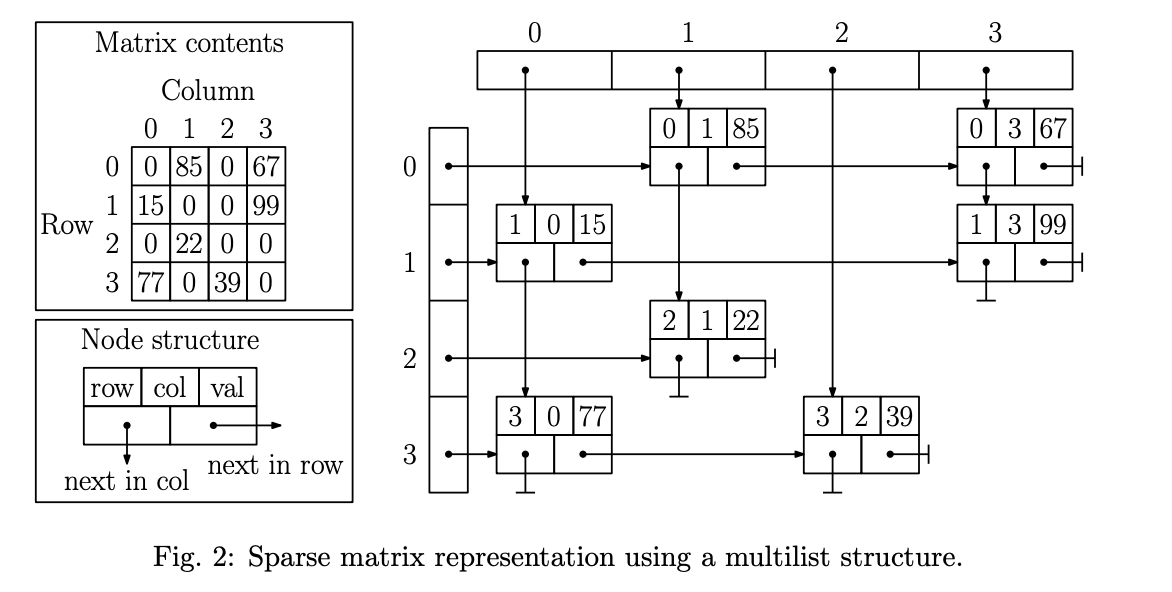
\includegraphics[scale=0.3]{Fig_2}
  \end{center}
  \subsection{Proof Amortized Cost}
  \textbf{Theorem:} When doubling array size for reallocation, amortized cost of list operation is $O(1)$.\\ \\
  \textbf{Proof:} Assume we are using a stack (can be proven for other ADT). Let $n$ be the current size of the array. Each time we push an element, we store an additional 4 tokens into a bank. Once the array is full, we reallocate an array of size $2n$ which requires intializing the array and copying elements (this will take $2n$). Last time we reallocated was when we transitioned from an array of size $n/2$ to $n$ so we must have performed at least $n - n/2 = n/2$ insertions. Now we have $4(n/2) = 2n$ from the extra tokens we stored. \\
  If we had instead added an additional $c$ spaces when we reallocated, there would be an issue when the table size becomes too large since reallocation would take a greater magnitude than the savings we collect.\\
  If we had instead raised the size of the array by a power, this works but we end up wasting a lot of space.
  \newpage
  \noindent\section{Trees}
  Free Tree: connected, undirected graph with no cycles (like MST)\\ \\
  Root Tree: each non-leaf node has $\geq$ 1 children and a single parent (except root)
  \setlist{nolistsep}
  \begin{itemize}[noitemsep]
  \item Aborescence = out-tree \quad Anti-arborescence = in-tree 
  \item Depth = max \# of edges of path from root to a node \\
  \end{itemize}
  \subsection{Tree Representation}
  Binary representation of a rooted tree: nodes have a pointer to first child and another pointer to next sibling
  \begin{center}
    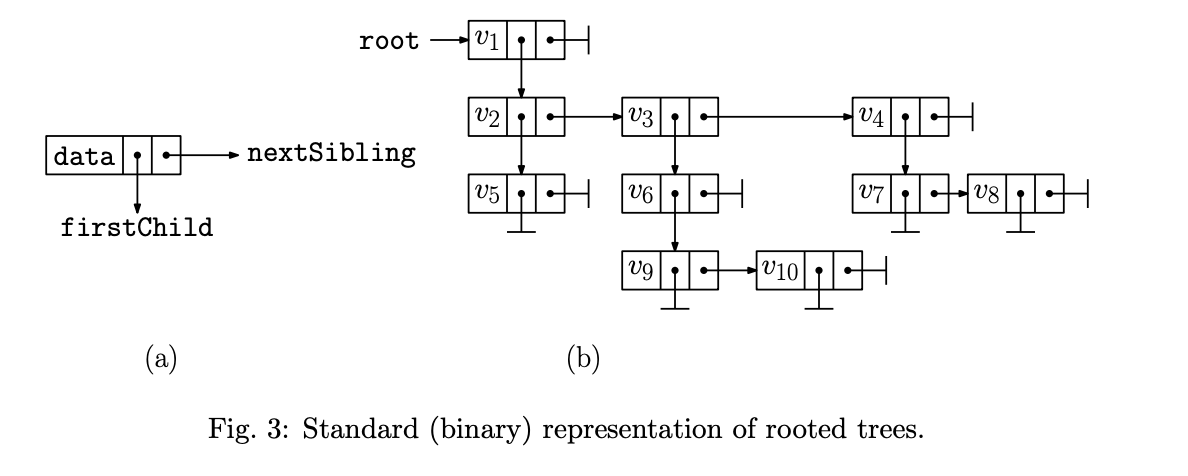
\includegraphics[scale=0.3]{Fig_3}
  \end{center}
  Binary Tree: rooted, ordered tree where each non-leaf node has 2 possible children (left, right)
  \setlist{nolistsep}
  \begin{itemize}[noitemsep]
  \item Full Tree: All nodes either have 0 children or 2 children
  \item Can make any binary tree a full binary tree by extending tree by adding external nodes to replace all empty subtrees
  \end{itemize}
  \begin{center}
  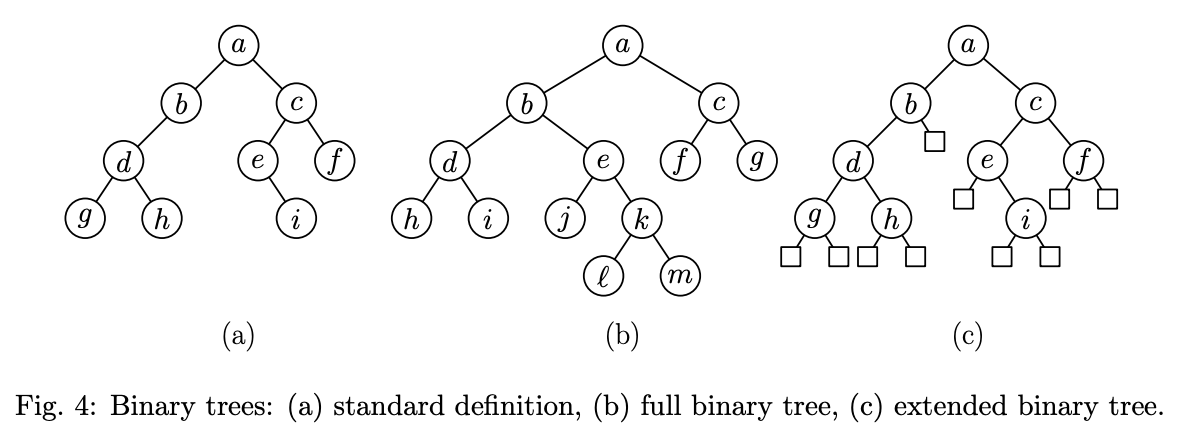
\includegraphics[scale=0.4]{Fig_4}
  \end{center}
  \begin{lstlisting}
    class BinaryTreeNode<E> {
      private E entry;
      private BinaryTreeNode<E> left;
      private BinaryTreeNode<E> right;
      ...
    }
  \end{lstlisting}
  In-order traversal: left, root, right \\
  Pre-order traversal: root, left, right \\ 
  Post-order traversal: left, right, root\\
  \newpage
  \subsection{Extended Binary Trees}
  If there are $n$ internal nodes, there are $n + 1$ external nodes. Quasi proof by noticing that we will essentially replace every leaf with 1 internal and 2 external nodes.\\  \\
  \textbf{Theorem: }If there are n internal nodes in an extended tree, there are n+1 external nodes\\ \\
  \textbf{Proof: } 
  \begin{itemize}[noitemsep]
  \item Proof by induction: Extended tree binary tree with n internal nodes has n+1 external nodes has 2n+1 total nodes
  \item Let x(n) = number of external nodes given n internal nodes and prove x(n) = n + 1
  \item Base Case x(0) = 1 a tree with no internal nodes has 1 external node
  \item IH: Assume x(i) = i + 1 for all i $\leq$ n - 1
  \item IS: let $n_{L}$ and $n_{R}$ be the number of nodes in Left and Right subtrees
  \item $x(n) = x(n_{L}) + x(n_{R}) = (n_{L} + 1) + (n_{R} + 1) = (1 + n_{L} + n_{R}) + 1 = n + 1$ external nodes
  \item so $n + 1$ (external) + $n$ (internal) = $2n + 1$
  \item Moreover, about 1/2 of nodes of extended Binary Tree are leaf nodes
  \end{itemize}
  \subsection{Threaded Binary Trees}
  Give null pointers information about where to traverse next
  \setlist{nolistsep}
  \begin{itemize}
  \item If left-child = null then stores reference to node's inorder predecessor
  \item If right-child = null then stores references to node's inorder successor
  \end{itemize}
  \begin{center}
  \includegraphics[scale=0.3]{Fig_6}
  \end{center}
  \begin{lstlisting}
    BinaryTreeNode inOrderSuccessor(BinaryTreeNode v) {
      BinaryTreeNode u = v.right;
      if(v.right.isThread) return u;
      while(!u.left.isThread) u = u.left;
      return u;
    }
  \end{lstlisting}
  To find the inorder successor of a node:
  \begin{itemize}[noitemsep]
  \item If v's right-child is a thread, then we follow thread.
  \item Otherwise go through v's right child and iterate through left-child links until we find the last node before the thread
  \end{itemize}
  \subsection{Complete Binary Tree}
  Represented using sequential allocation (array) because no space is wasted
  \begin{itemize}[noitemsep]
  \item number of nodes is inbetween $2^{h}$ and $2^{h+1}-1$
  \end{itemize}
  \begin{lstlisting}
    leftChild(i): if(2i <= n) then 2i else null;
    rightChild(i): if (2i + 1 <= n) then 2i + 1 else null;
    parent(i): if (i >= 2) then [i/2] else null;
  \end{lstlisting}
  \newpage
  \section{Dictionaries}
  \begin{lstlisting}
    void insert(Key x, Value v) // if key exists, exception is thrown 
    void delete(Key x) // if key does not exist, exception thrown 
    Value find(Key x) // return value associated with key or null if not found
  \end{lstlisting}
  \subsection{Array Representation}
  \begin{itemize}[noitemsep]
  \item Unsorted Array has O(n) search and delete, O(n) because we need to check for duplicates
  \item Sorted Array has O(logn) search and O(n) insertion and deletion because when we modify the array we need to shift elements
  \end{itemize}
  \subsection{Binary Search Tree Representation}
  Search: O(n) for degenerate tree, O(logn) for balanced tree \\
  Can use extended BST to give info about how the target key is inbetween its inorder predecessor and inorder successor
  \begin{lstlisting}
    //Recursive
    Value find(Key x, BinaryNode p) {
      if (p == null) return null;
      else if (x < p.key) return find(x, p.left);
      else if (x > p.key) return find(x, p.right);
      else return p.val;
    }

    //Iterative
    Value find(Key x) {
      BinaryNode p = root;
      while(p != null) {
        if (x < p.key) p = p.left;
        else if (x > p.key) p = p.right;
        else return p.value;
      }
      return null;
    }
  \end{lstlisting}
  Insert: search for key and if found throw exception else we hit a null and insert there 
  \begin{itemize}[noitemsep]
  \item Either tree is empty so return new node or we return the root of the original tree with the added node
  \item O(n) insert for degenerate tree, O(logn) insert for balanced tree
  \end{itemize}
  \begin{lstlisting}
    BinaryNode insert(Key x, Value v, BinaryNode p) {
      if (p == null) p = new BinaryNode(x, v, null, null);
      else if (x < p.key) p.left = insert(x, v, p.left);
      else if (x > p.key) p.right = insert(x, v, p.right);
      else throw DuplicateKeyException;
      return p;
    }
  \end{lstlisting}
  \newpage
  \noindent Delete: 
  \begin{itemize}[noitemsep]
    \item if target node is a leaf, remove it
    \item if target node only has 1 child, replace it with the child
    \item else replace target node with inorder successor (aka leftmost on right subtree). End the delete the replacement node
  \end{itemize} 
  \begin{lstlisting} 
    BinaryNode delete(Key x, BinaryNode p) {
      if (p == null) throw KeyNotFoundException;
      else 
        if (x < p.data)
          x.left = delete(x, p.left);
        else if (x > p.data)
          x.right = delete(x, p.right)
        else if (p.left == null || p.right == null) 
          if (p.left == null) return p.right;
          else return p.left;
        else 
          r = findReplacement(p);
          //copy r's contents to p
          p.right = delete(r.key, p.right);
    }

    BinaryNode findReplacement(BinaryNode p) {
      BinaryNode r = p.right;
      while(r.left != null) r = r.left;
      return ;
    }
  \end{lstlisting}
  \subsection{Analysis of BST}
  O(n) deletion for degenerate tree, O(logn) deletion for balanced tree\\ \\
  \textbf{Theorem: } Height of BST on average will be ln(n). \\ \\
  \textbf{Proof: } 
  \begin{itemize}[noitemsep]
  \item for i = 2 to n, insert elements into BST and look at depth of left most node (min value)
  \item chance that a number is the min is $\frac{1}{i}$ so Expected Height is $\sum_{i=2}^{n} \frac{1}{i}$ $\approx$ ln(n)
  \end{itemize}
  \subsection{Random Insertions and Deletions on BST}
  Because the replacement node will always be the inorder successor, if we repeatedly add and remove random elements from a BST, this biased choice will eventually bring the height of the tree to $O(\sqrt{n})$\\
  This bias can be handled by randomly selecting the replacement node as the inorder successor or the inorder predecessor
  \newpage
  \section{AVL Trees}
  \textbf{AVL Balance Condition: }For every node in tree, absolute difference between heights of left and right subtrees is at most 1. A node's balance factor is determined by
  \begin{center}
    balance(v) = height(v.right) - height(v.left)
  \end{center}
  Worst case height can be shown to be O(logn) using Fibonacci sequence
  \begin{itemize}[noitemsep]
  \item $F_{h} \approx \varphi^{h}\sqrt{5}$ where $\varphi = (1 + \sqrt{5})/2$ 
  \item let N(h) denote minimum number of nodes in any AVL tree of height h. So 1 child will have height h-1 and the other will have height h-2
  \item N(0) = 1, N(1) = 2, N(h) = 1 + $N(h_{L}) + N(h_{R}) = 1 + N(h-1) + N(h-2)$
  \item Now $N(h) = n \geq c \varphi^{h} \rightarrow h \leq log_{\varphi}n \rightarrow h = O(logn)$
  \item Also find method using AVL is O(logn)
  \end{itemize}
  \begin{center}
  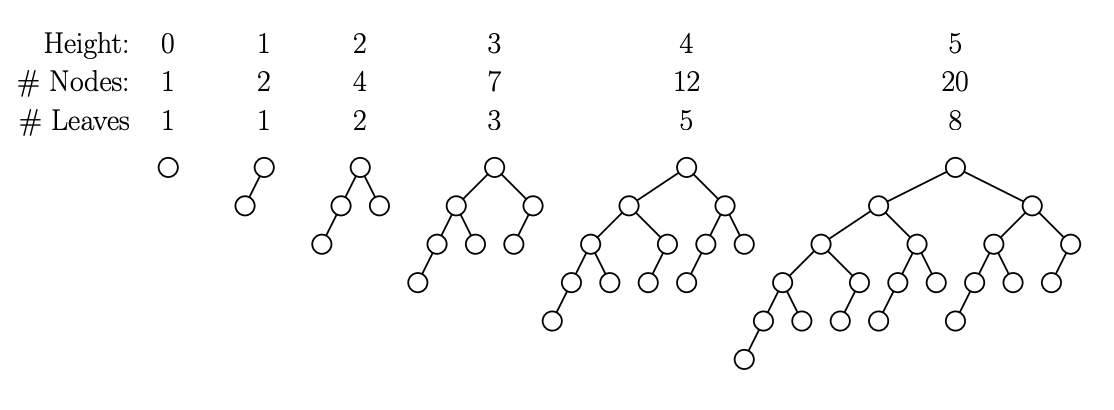
\includegraphics[scale=0.3]{FibTreeMinNodes}
  \end{center}
  Rotations are used to main tree's balance by modifying relation between two nodes but preserving the tree's inorder properties 
  \begin{lstlisting}
    BinaryNode rotateRight(BinaryNode p) {
      BinaryNode q = p.left;
      p.left = q.right;
      q.right = p;
      return q;   // q is now root
    }
    Binary Node rotateLeft(Binary Node p) {
      BinaryNode q = p.right;
      p.right = q.left;
      q.left = p;
      return q;   // q is now root
    }
  \end{lstlisting}
  \begin{center}
  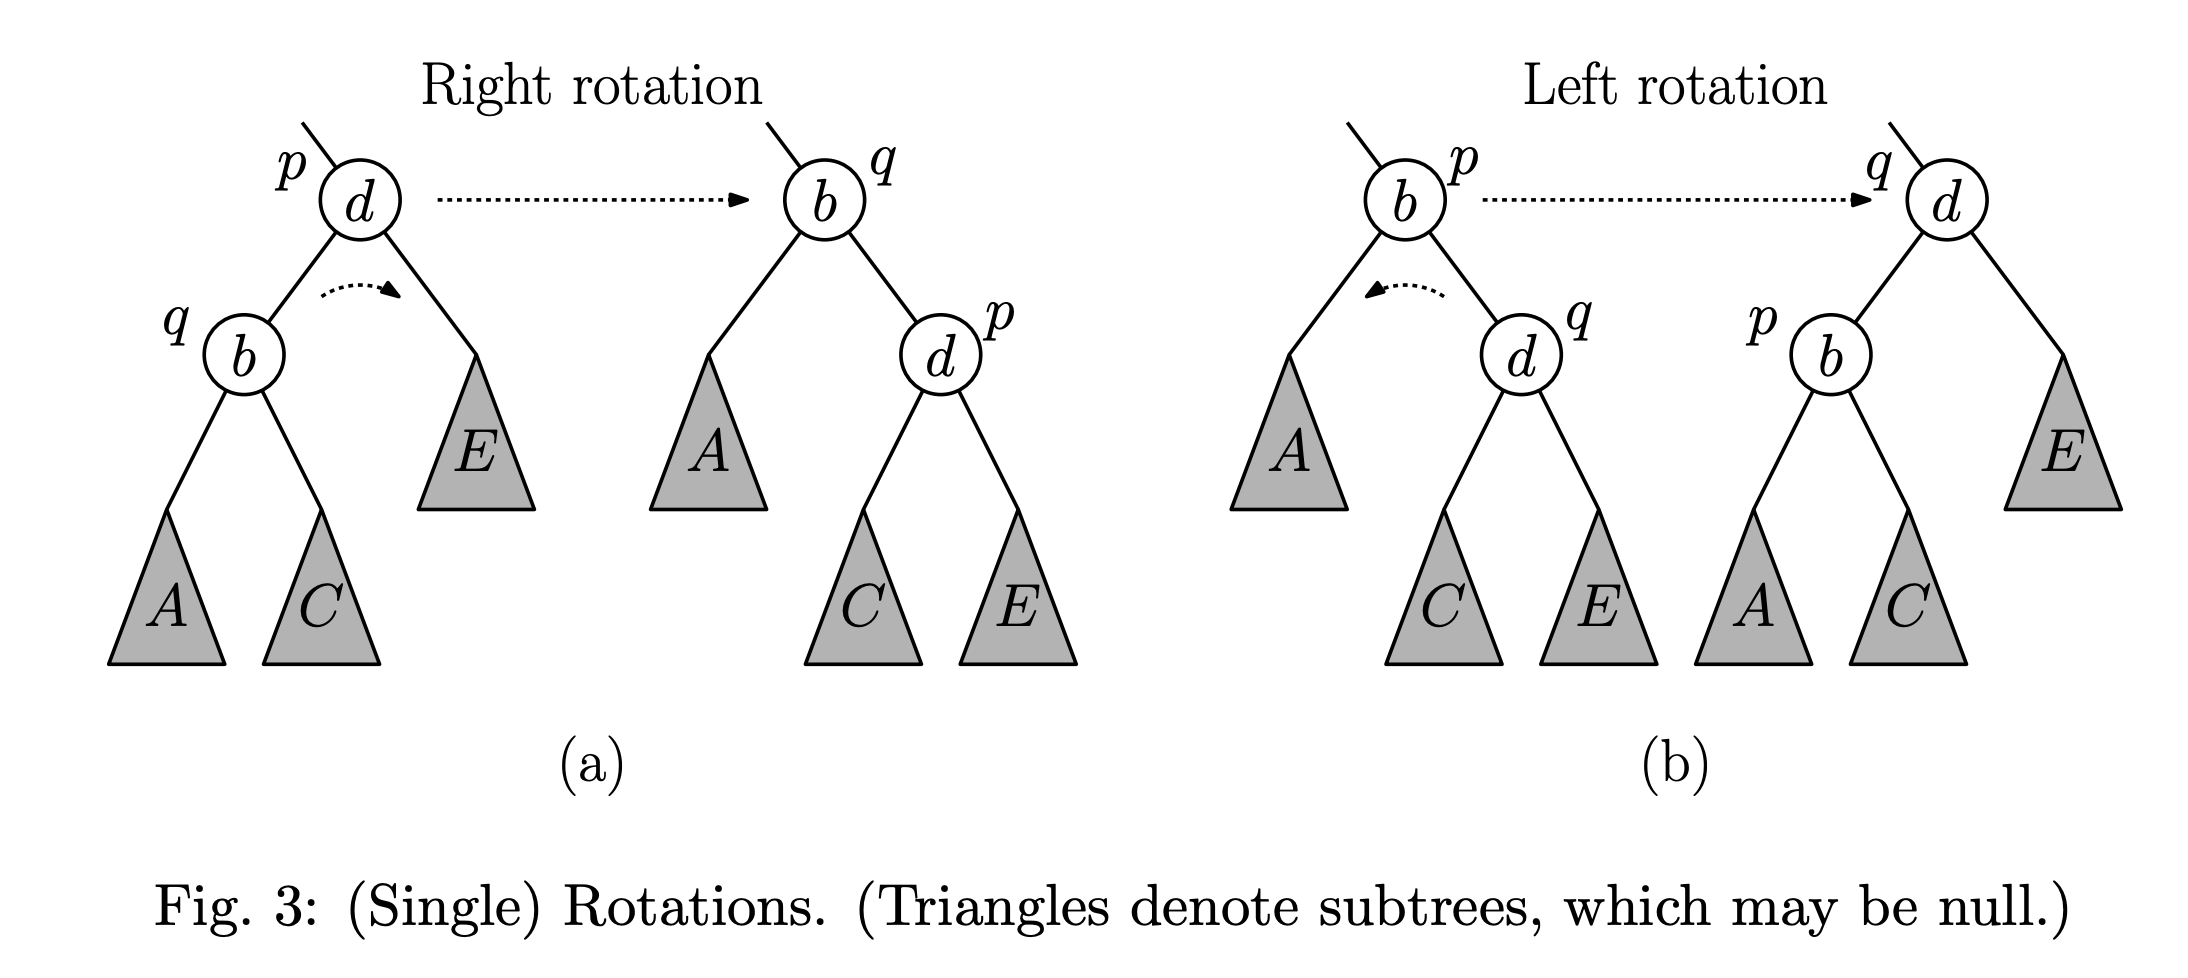
\includegraphics[scale=0.15]{FibTreeRotation}
  \end{center}
  \newpage
  Single rotations work when the imbalance occurs on the outer edges of the tree. Need to use double rotations LR or RL to balance inner trees \\
  \begin{center}
  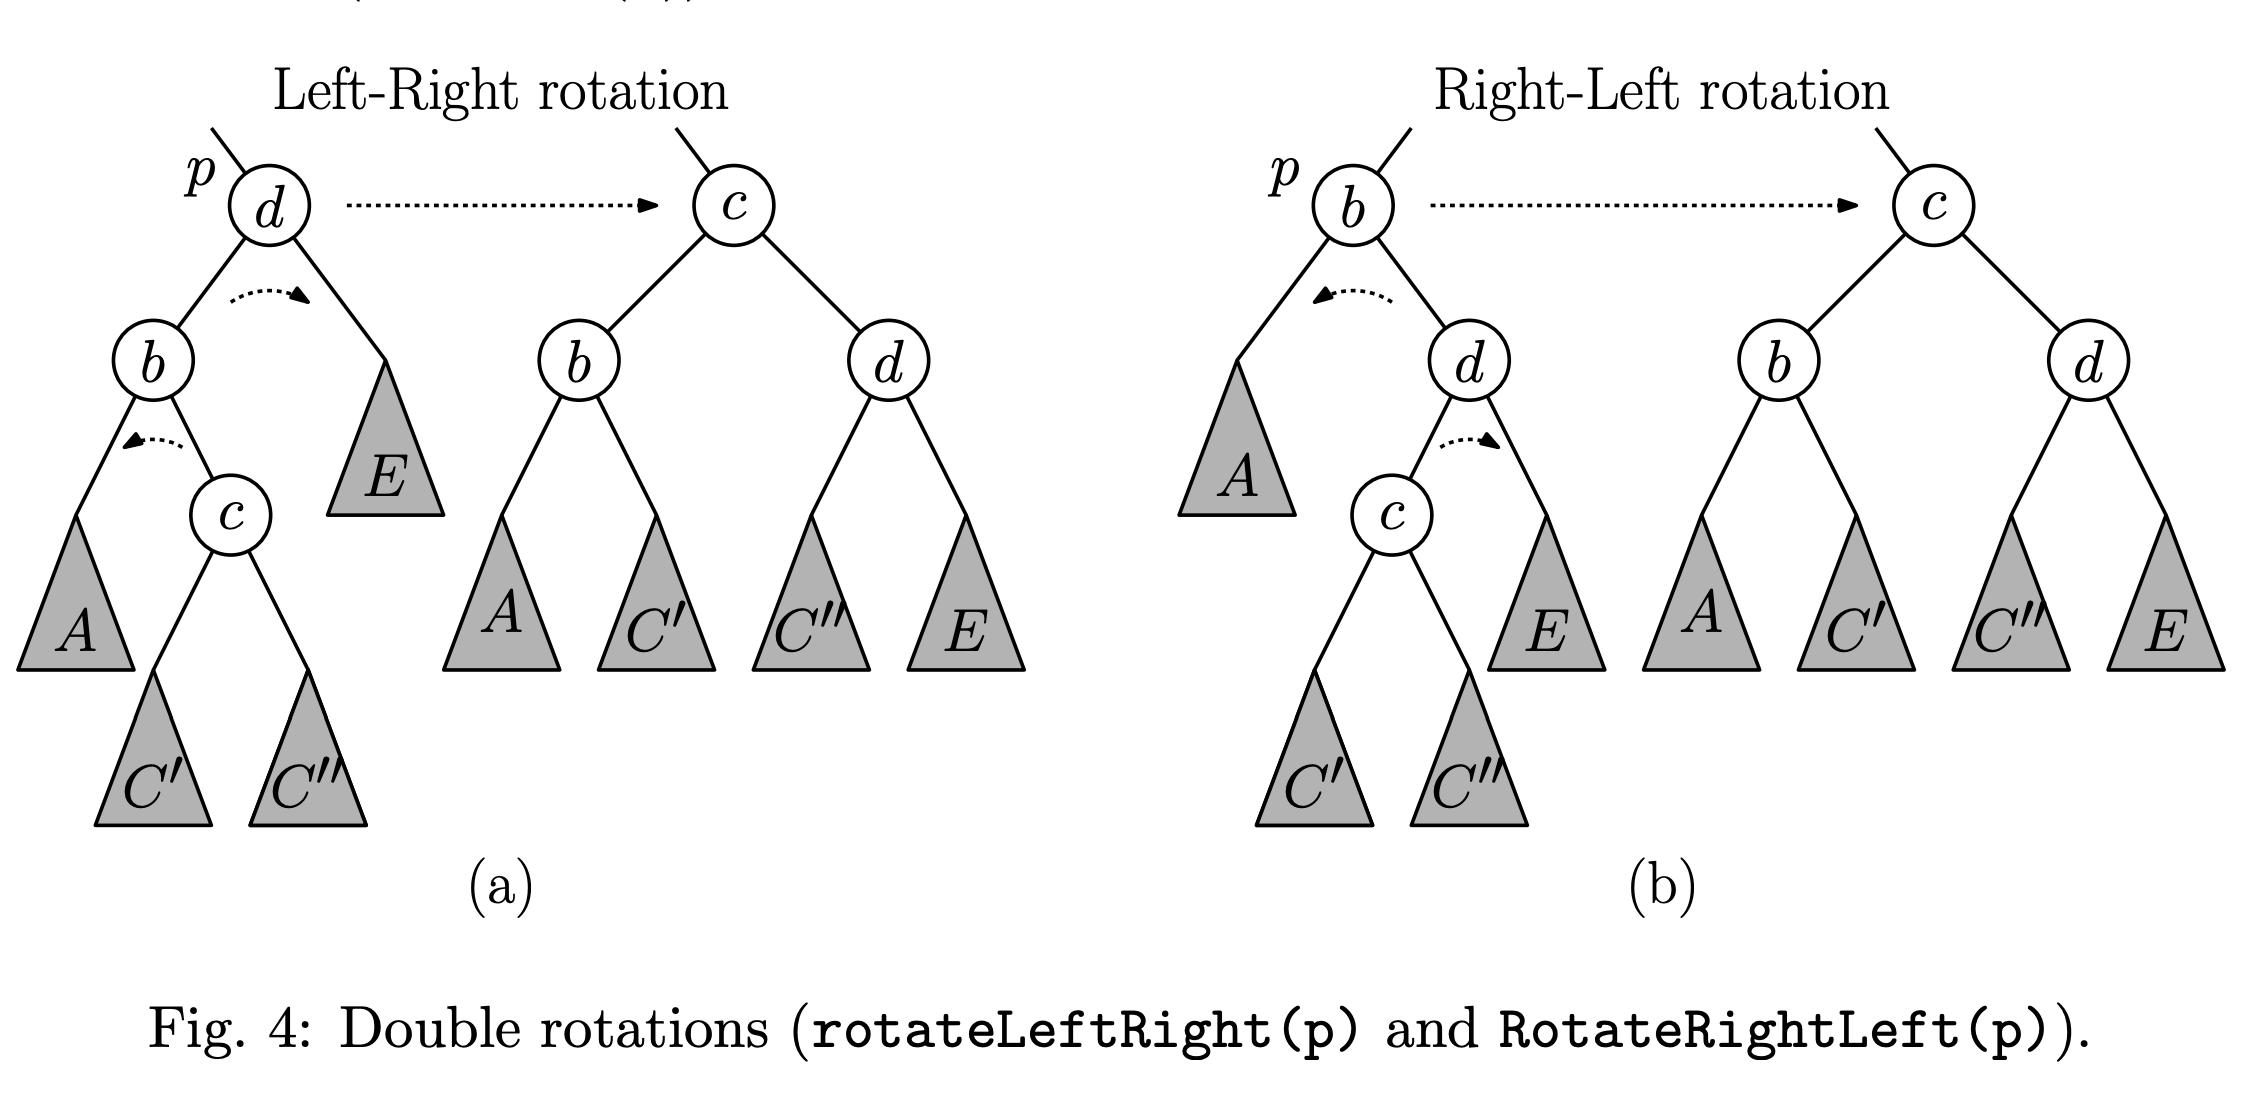
\includegraphics[scale=0.15]{FibTreeDoubleRotation}
  \end{center}
  Insertion works similar to BST except we update the heights of subtrees and apply rotations to maintain height \\
  When insertion occurs balance factors of ancestors is altered by $\pm$1\\
  If a node has a balance factor that violates Balance Property:
  \begin{itemize}[noitemsep]
  \item Left-Left substree too deep then rotate right on unbalanced node
  \item Right-Right subtree too deep then rotate left on unbalanced node
  \item Left-Right subtree too deep then rotate left-right (left child of unbalanced node then unbalanced node)
  \item Right-Left subtree too deep then rotate right-left (right child of unbalanced node then unbalanced node)
  \end{itemize}
  \begin{center}
  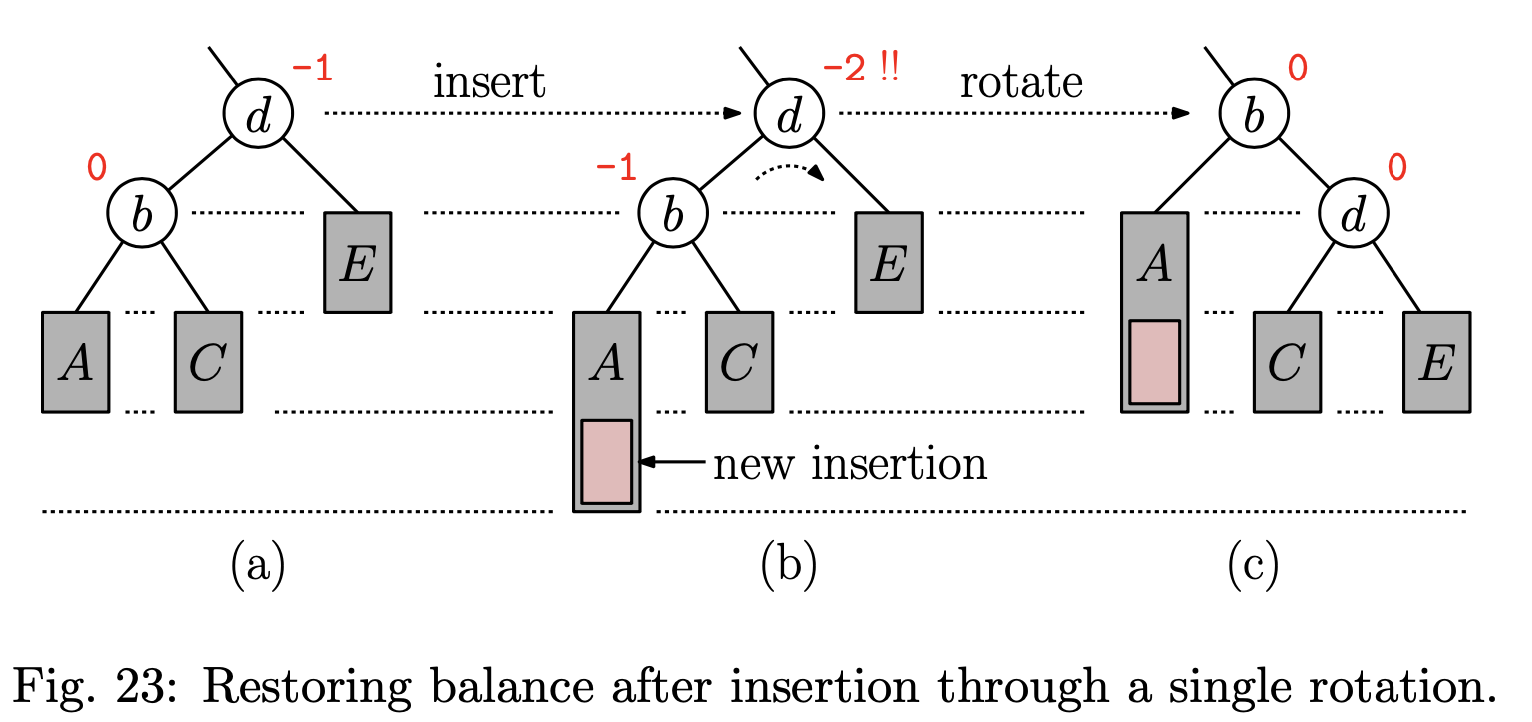
\includegraphics[scale=0.4]{AVLSingleRotationInsertion}
  \end{center}
  \begin{center}
  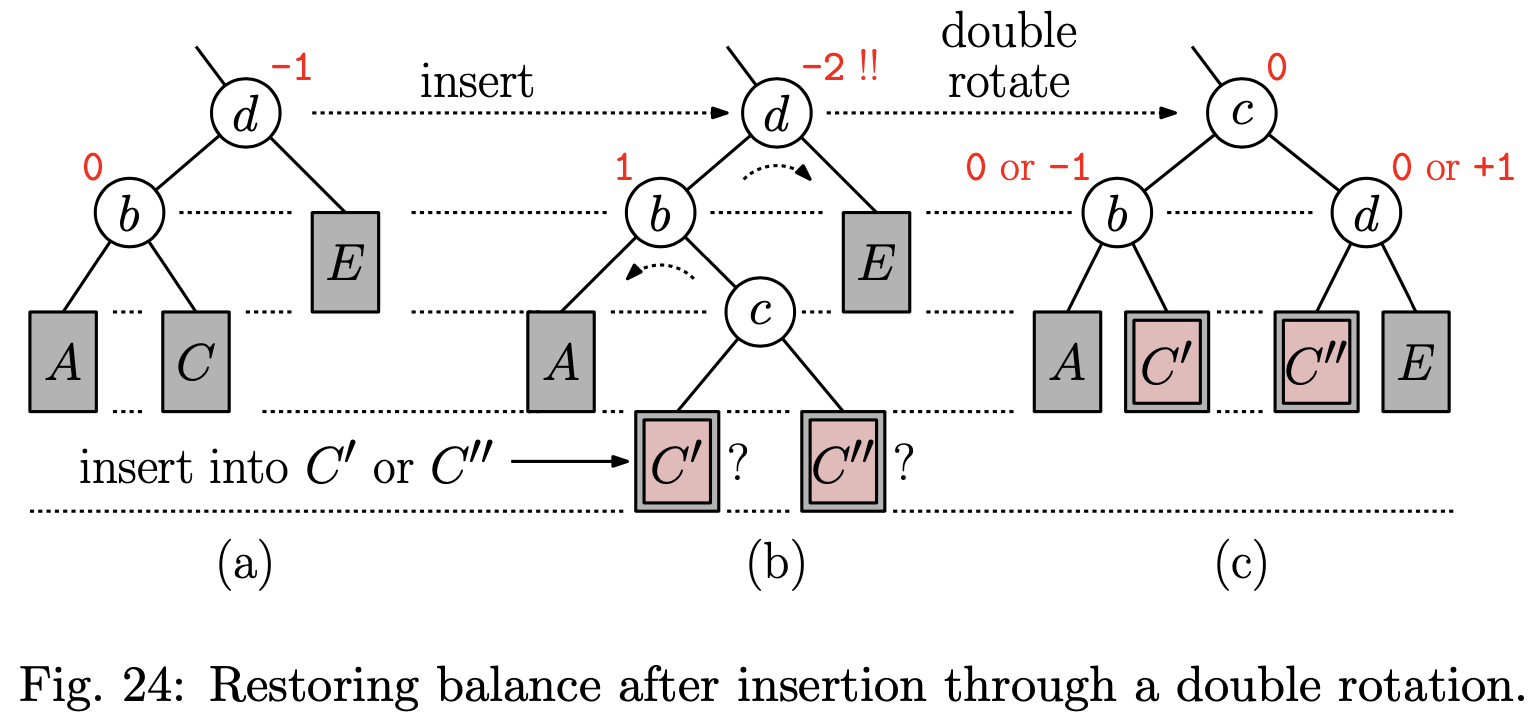
\includegraphics[scale=0.4]{AVLDoubleRotationInsertion}
  \end{center}
  \newpage
  \begin{lstlisting}
    int height(AvlNode p) return p == null ? -1 : p.height;
    void updateHeight(AvlNode p) p.height = 1 + max(height(p.left), height(p.right));
    int balanceFactor(AvlNode P) return height(p.right) - height(p.left);
    AvlNode rotateRight(AvlNode p) {
      AvlNode q = p.left;
      p.left = q.right;   // swap inner child
      q.right = p;        // bring q above p
      updateHeight(p);
      updateHeight(q);
      return q;           // q replaces p
    }
    AvlNode rotateLeft(AvlNode p) {... symmetrical to rotateRight ...}
    AvlNode rotateLeftRight(AvlNode p) {
      p.left = rotateLeft(p.left);
      return rotateRight(p);
    }
    AvlNode rotateRightLeft(AvlNode p) {... symmetrical to rotateLeftRight ...}
    AvlNode insert(Key x, Value v, AvlNode p) {
      if (p == null) p = newAvlNode(x, v, null, null);
      else if (x < p .key) p.left = insert(x, v, p.left);
      else if (x > p.key) p.right = insert(x, v, p.right);
      else throw DuplicateKeyException;
      return rebalance(p);
    }
    AvlNode rebalance(AvlNode p) {
      if (p == null) return p;
      if (balanceFactor(p) < -1) {
        if (height(p.left.left) > height(p.left.right)) {//left-left heavy
          p = rotateRight(p);
        } else {                                          //left-right heavy
          p = rotateLeftRight(p);
        }
      }
      else if (balanceFactor(p) > 1) {
        if(height(p.right.right) > height(p.right.left)) {//right-right heavy
          p = rotateLeft(p);
        } else {                                            //right-left heavy
          p = rotateRightLeft(p);
        }
      }
      updateHeight(p);
      return p;
    }
  \end{lstlisting}
  \newpage
  Deletion works in a similar manner in that we call normal BST delete and then rotate as necessary. However we need to call rebalance on further ancestors to check balance condition (e.g. if one of the inner subtrees is too tall, we need to call a double rotation)
  \begin{center}
  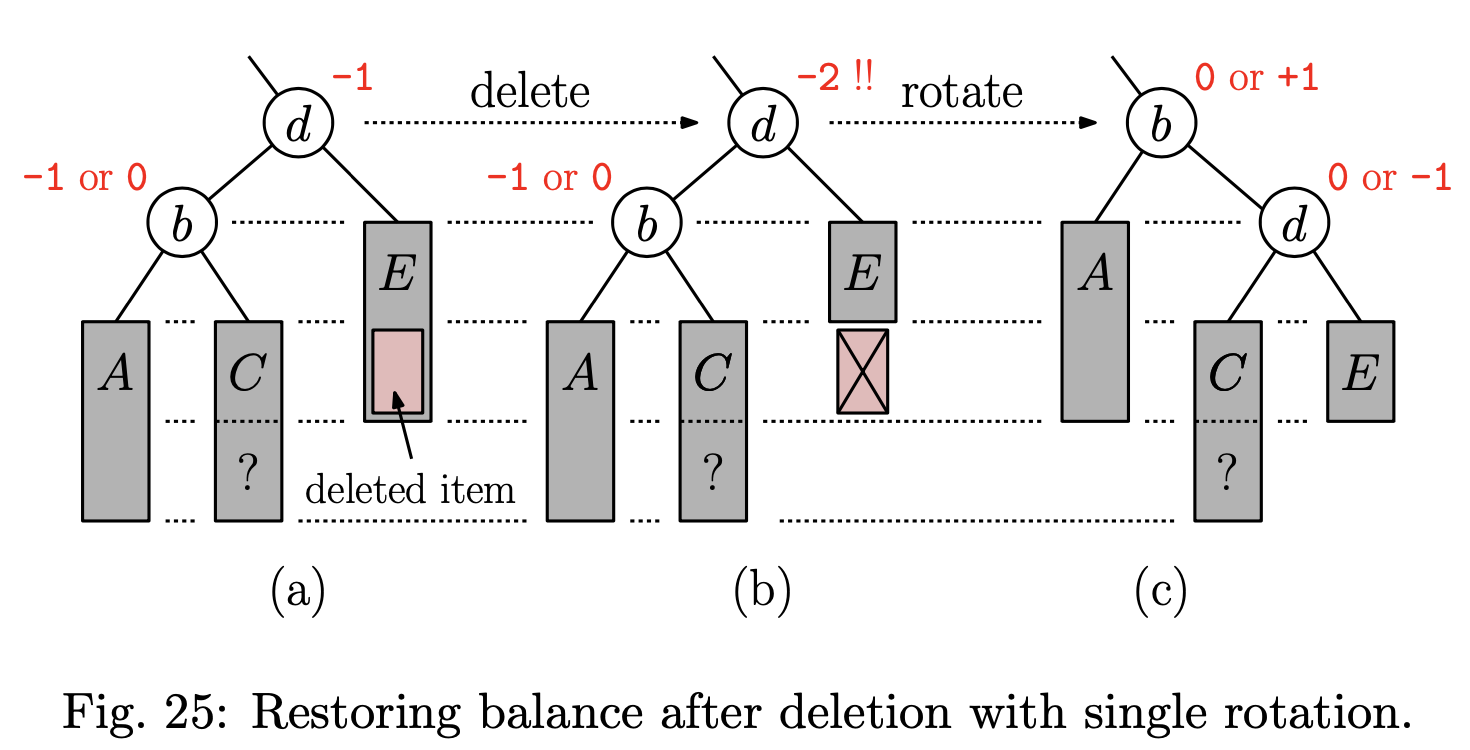
\includegraphics[scale=0.4]{AVLSingleRotationDeletion}
  \end{center}
  \begin{center}
  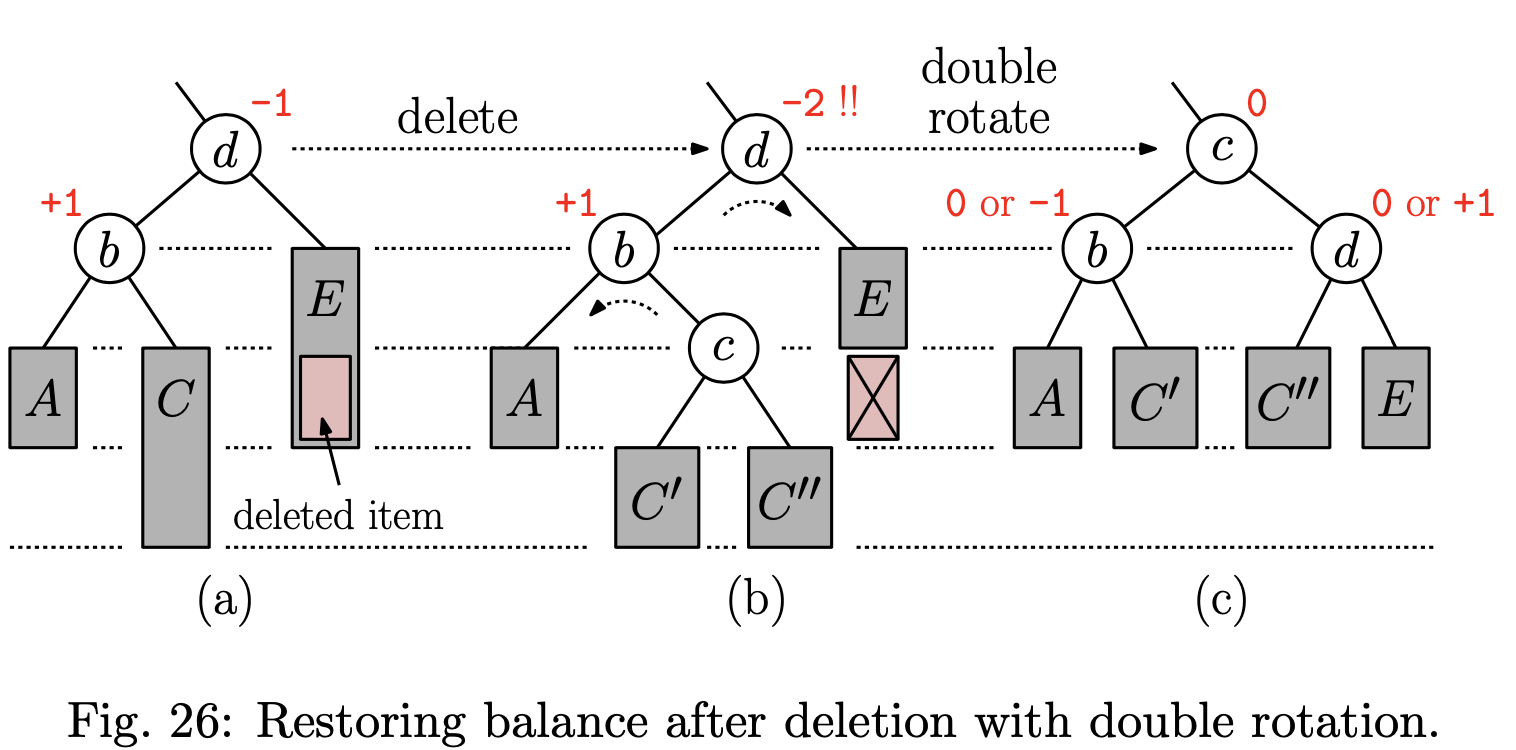
\includegraphics[scale=0.4]{AVLDoubleRotationDeletion}
  \end{center}
  Note that node d dropped one level so we need to call balance check on c. In this case deletion can end up calling a cascade of O(logn) rebalancing operations
  \newpage 
  \section{2-3 Trees, Red-Black Trees, AA Trees}
  \subsection{2-3 Trees}
  Nodes can either be 2-node (normal binary tree) or 3-node (2 keys b,d and 3 branches A, C, E where A $<$ b $<$ X $<$ d $<$ E)
  Important thing to note is that all leaves are on the same level
  \begin{center}
  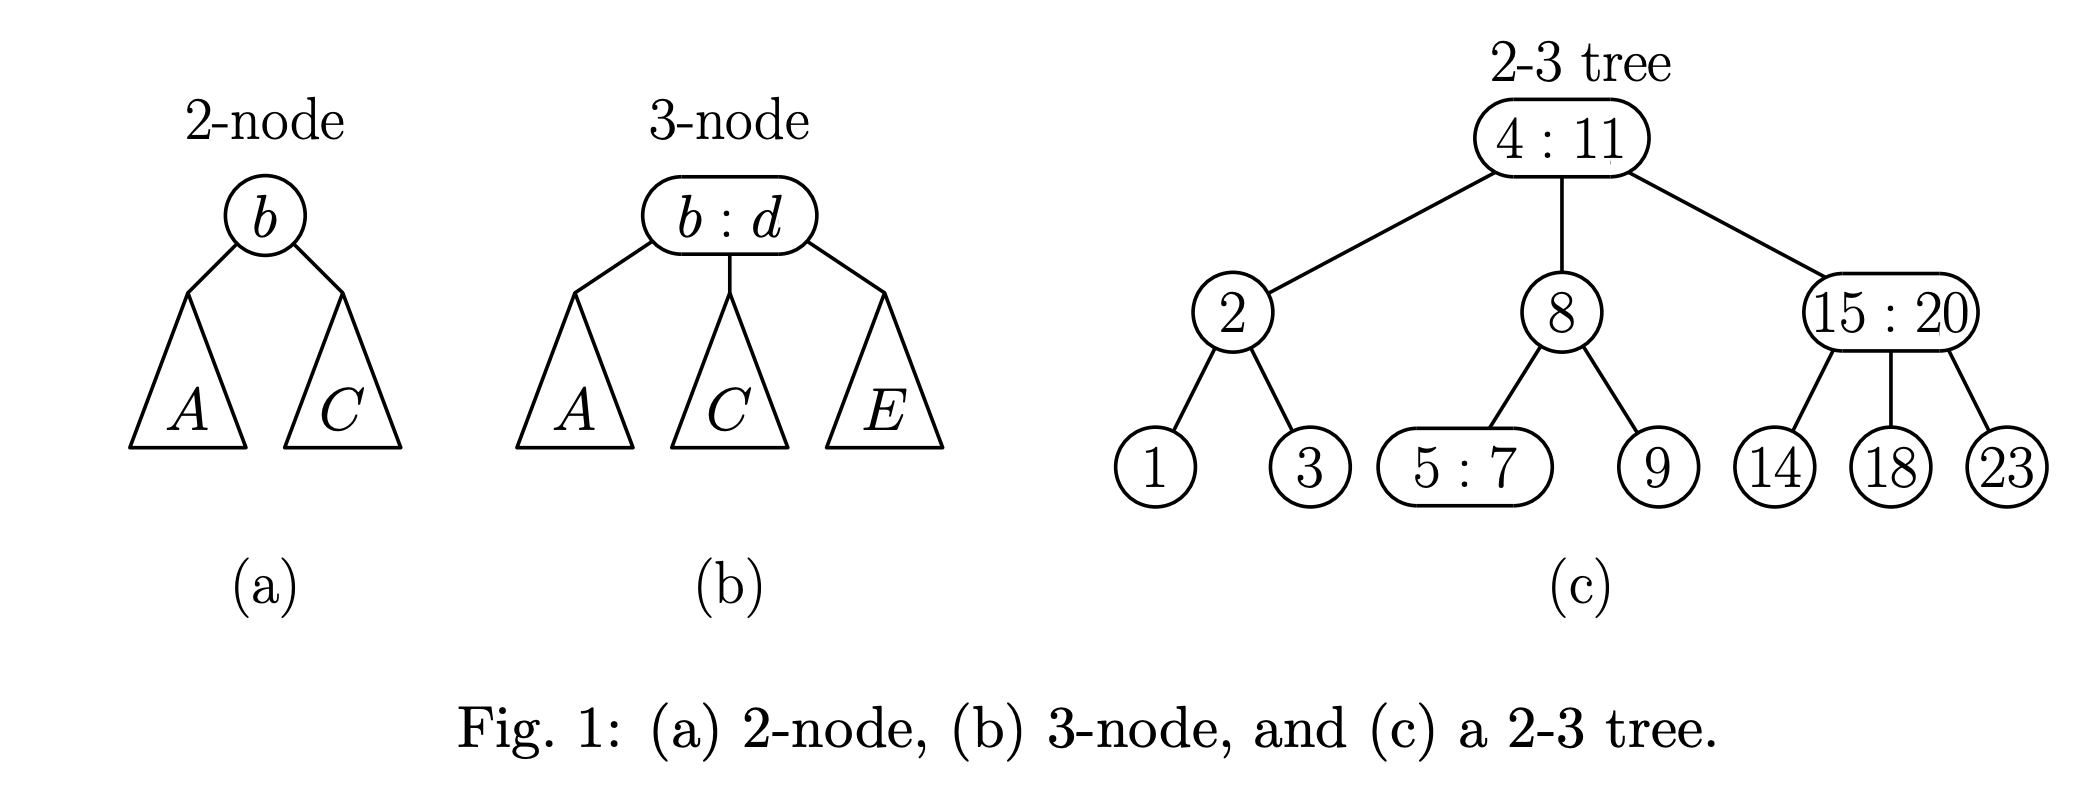
\includegraphics[scale=0.2]{2-3Tree}
  \end{center}
  Recursively defined as:
  \begin{itemize}[noitemsep]
  \item empty (null)
  \item root is 2-node and has two 2-3 subtrees of equal height
  \item root is 3-node and has three 2-3 subtrees of equal height
  \end{itemize}
  Sparsest 2-3 tree is a complete binary tree \\ \\
  \textbf{Find: }recursive descent but when 3-node is reached, compare x with both keys to find which branch to go to\\ \\
  \textbf{Insertion: }search for key and and insert like in a normal tree.
  \begin{itemize}[noitemsep]
  \item if parent is a 2-node, now it is a 3-node with an added null subtree
  \item if parent is 3-node then it becomes 4-node (3 keys and 4 subtrees) and we have to fix it by splitting the 4-node into two 2-nodes and prop the middle key up for recursion and will continue to recurse up until it reaches  a 2-tree or the root
  \end{itemize}
  \begin{center}
  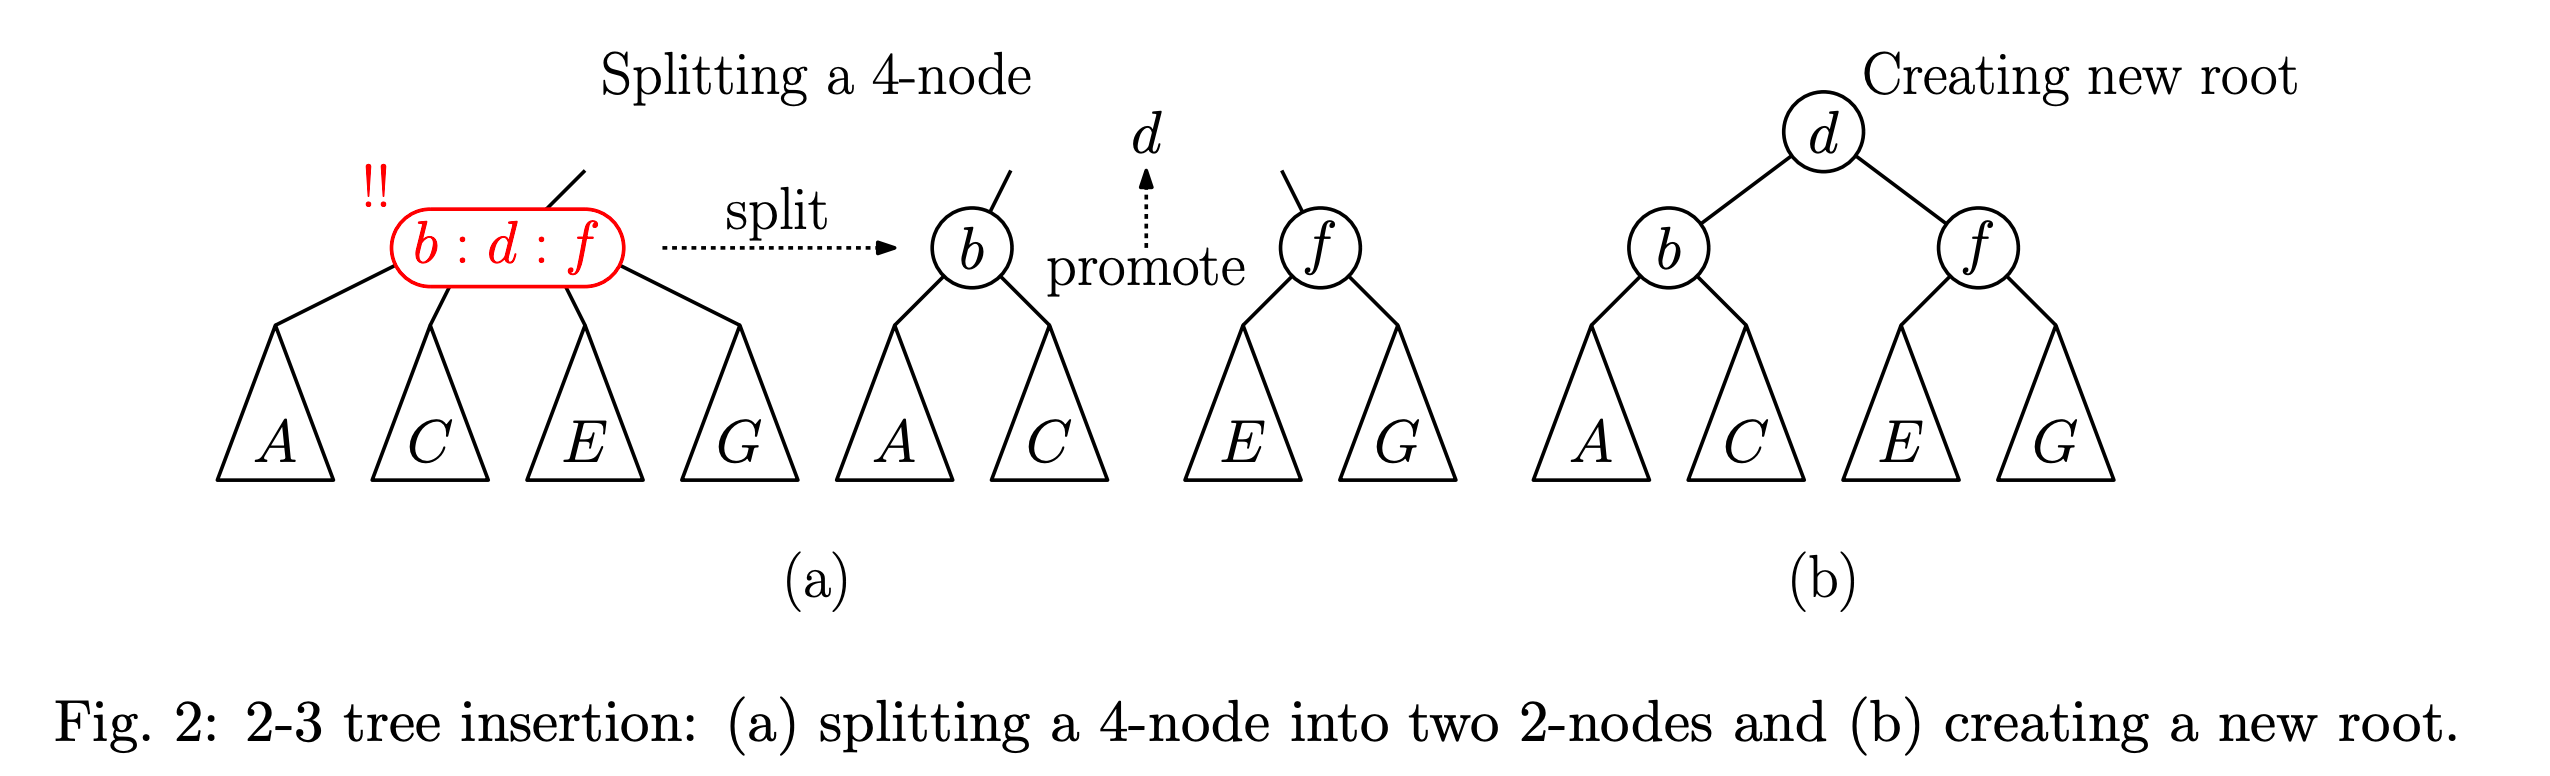
\includegraphics[scale=0.2]{2-3TreeInsert}
  \end{center}
  \newpage
  \textbf{Deletion: }find and replace target with inorder successor and then delete the leaf
  \begin{itemize}[noitemsep]
  \item If parent of leaf is a 3-node then parent becomes a 2-node and done
  \item If parent is a 2-node then it becomes a 1-node (0 keys, 1 subtree) so we can do
    \begin{itemize}[noitemsep]
      \item \textbf{Adoption: }if sibling is a 3-node then adopt a key and a subtree so we have two 2-nodes (this ends up being a rotation on the parent)
      \item \textbf{Merge: }merge 1-node and sibling 2-node and take a key from parent then recurse up. If root is reached and ends up being a 1-node, remove it and make its child the new root
    \end{itemize}
  \end{itemize}
  \begin{center}
    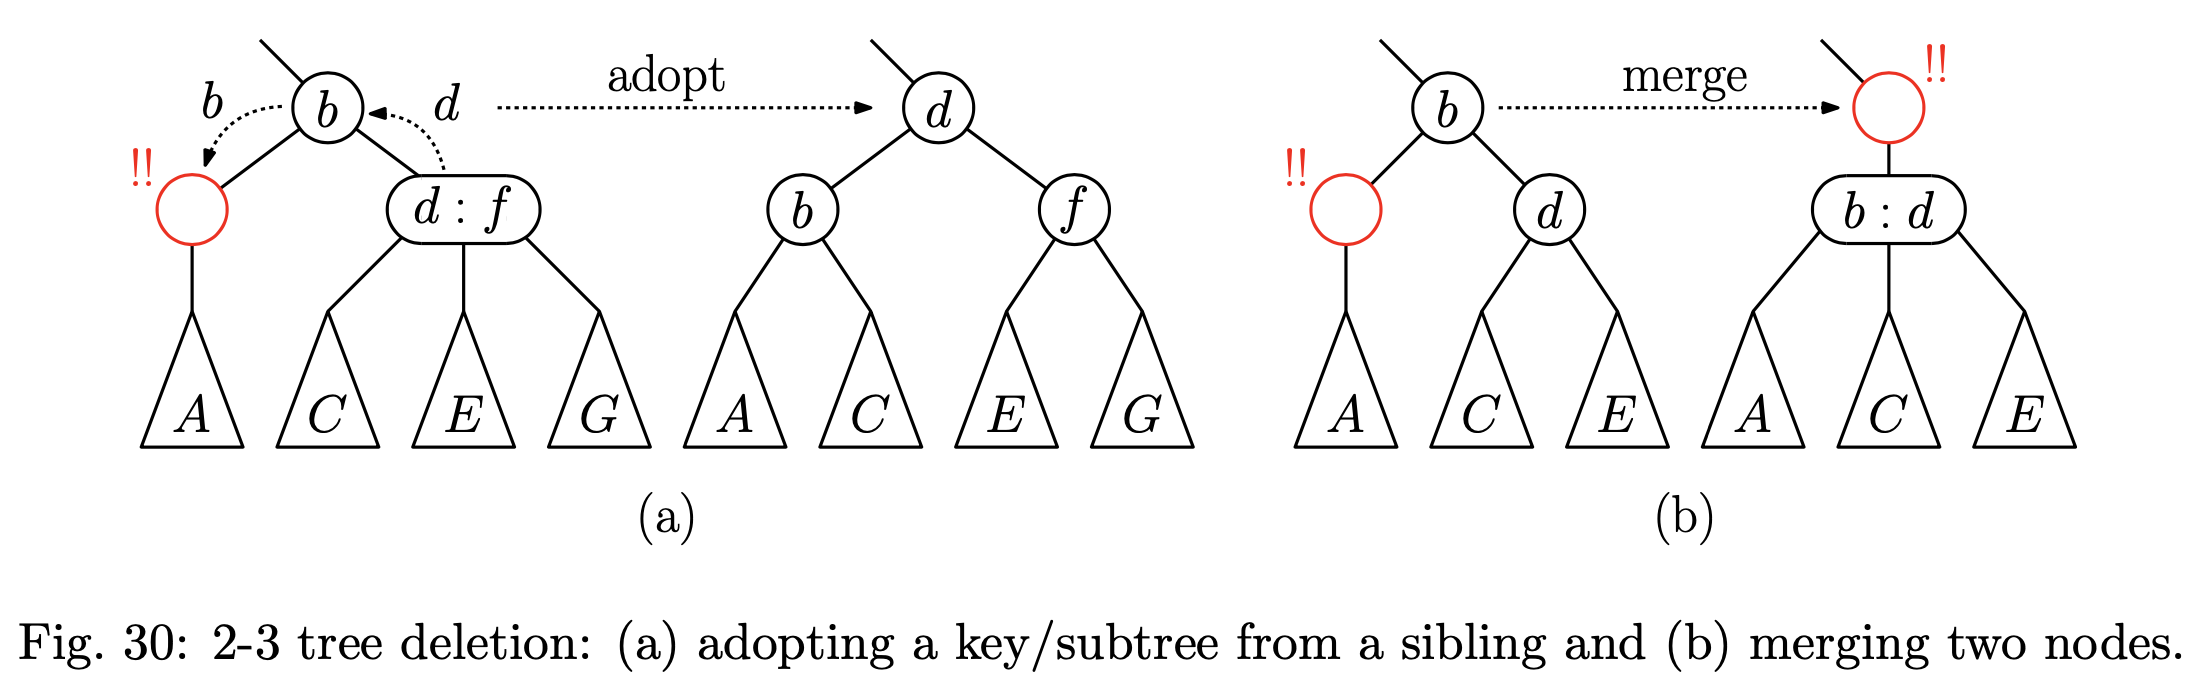
\includegraphics[scale=0.5]{2-3TreeAdoptAndMerge}
  \end{center}
  \subsection{Red-Black Trees}
  Take a 3-node and create a 2-node combo by using d, C, E as the right subtree and b, A for left subtree
  \begin{center}
  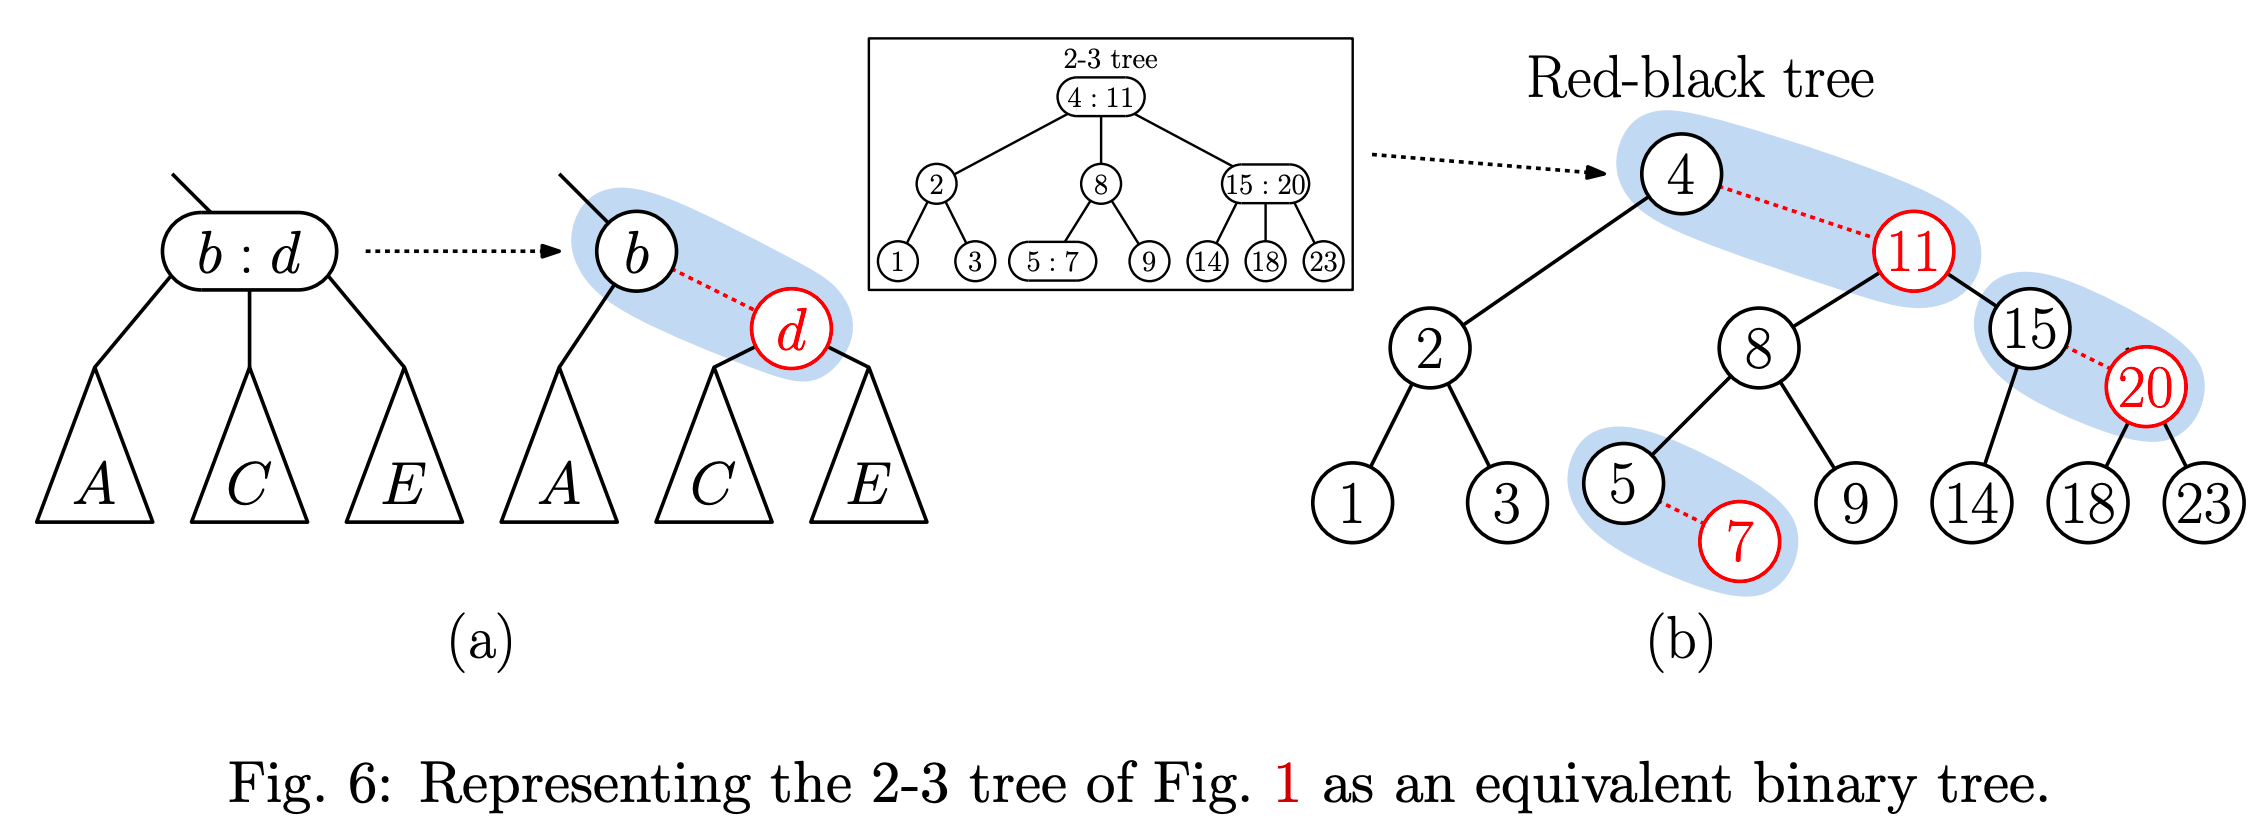
\includegraphics[scale=0.2]{RBTree}
  \end{center}
  Created right subnode is labeled red and all other nodes black, creating a binary search tree\\
  Null pointers are labeled black and if a node is red, then both its children must be black \\
  Every path from a given node to any of its null descendants contains the same number of black nodes\\ \\
  \textbf{Theorem: }Every 2-3 tree corresponds to a red-black tree but converse is not true
  \begin{itemize}[noitemsep]
  \item Issue with RB tree doesn't distinguish between L and R children so 3-node can be encoded in 2 different ways
  \item Also can't convert a node with 2 red children to 2-3 tree which ends up being a 4-node
  \end{itemize}
  \begin{center}
  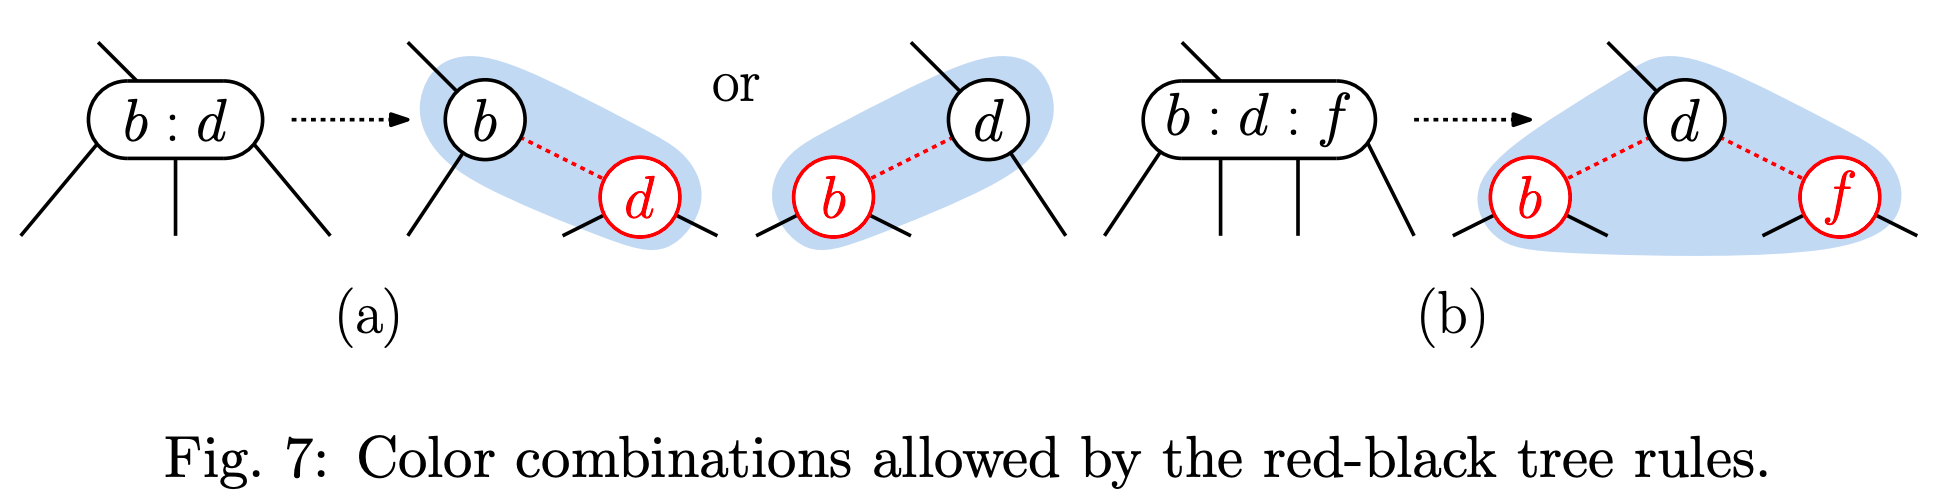
\includegraphics[scale=0.15]{2-3ToRBTree}
  \end{center}
  \subsection{AA Trees}
  Simplified RB tree where red nodes can only appear as right children of black nodes allowing conversion between 2-3 tree and RB trees \\
  Edge between red node and the black parent is called a red edge \\
  Implementation of AA trees also uses a sentinel node nil where every null pointer is replaced with a pointer to nil
  \begin{itemize}[noitemsep]
  \item In this case, nil.left == nil.right == nil so we don't have to keep doing null checks
  \end{itemize}
  Implementation of AA doesn't store colors. Instead stores level of associated node in 2-3 tree
  \begin{itemize}[noitemsep]
  \item nil = level 0
  \item If black, p.level = q.level (child) + 1
  \item If red, then same level as parent. Now can easily test if node is read by comparing with parent level
  \end{itemize}
  \begin{center}
  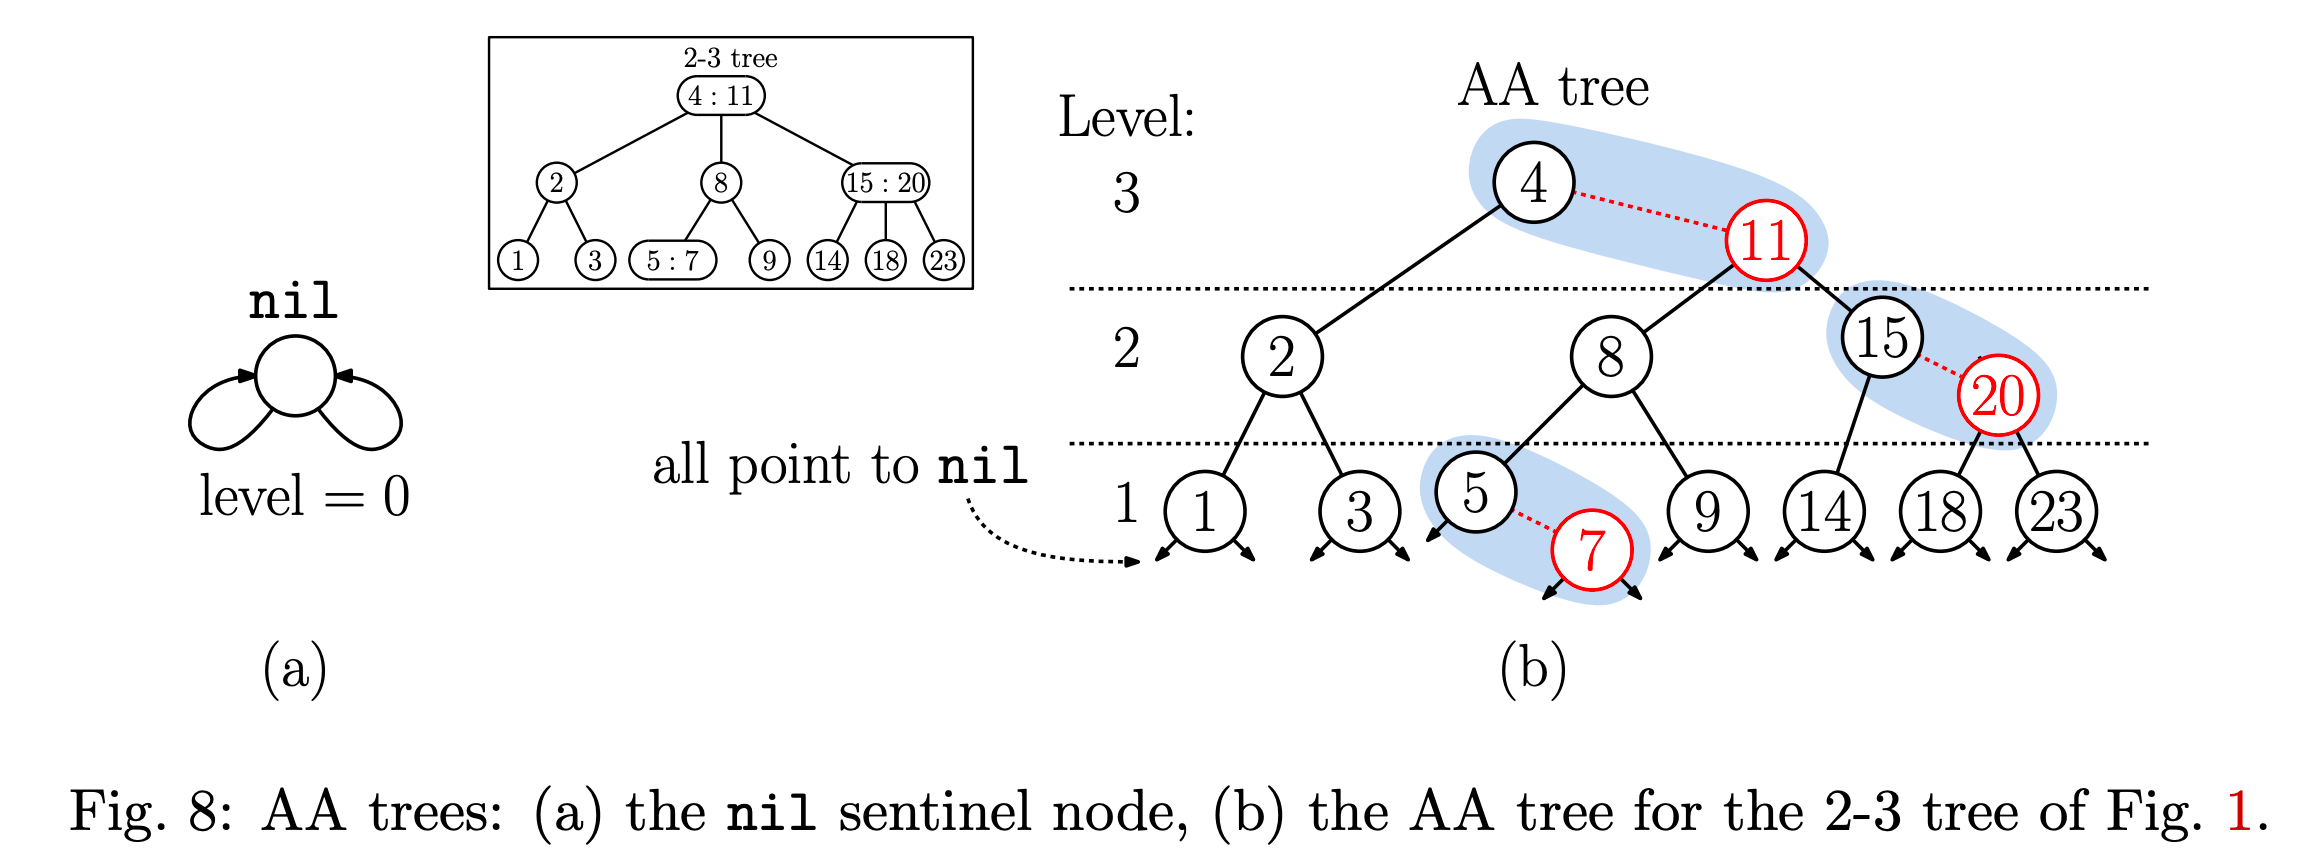
\includegraphics[scale=0.20]{AATree}
  \end{center}
  \textbf{Find: }works exactly the same as it does for BST \\ \\
  Insertion and Deletion require skew(p) and split(p)
  \begin{itemize}[noitemsep]
    \item \textbf{skew(p)} if p has a red left child, rotate right so red child is on right side
    \item \textbf{split(p)} if p has a red right-right chain, do a left rotation \& promote first red child to next level
  \end{itemize}
  Important thing to note is that p can either be black or red. If it is red we may need to recurse up to maintain AA tree invariant
  \begin{lstlisting}
    AANode skew(AANode p) {   
      if (p.left.level == p.level) {  // red node to our left?
        AANode q = p.left;            // do right rotation at p
        p.left = q.right;
        q.right = p;
        return q;
      }
      else return p;
    }
    AANode split(AANode p) {
      if (p.right.right.level == p.level) {   //right-right red chain?
        AANode q = p.right;                   // do left rotation at p
        p.right = q.left;
        q.left = p;
        q.level += 1;                         // promote q to higher level
        return q;
      }
      else return p;
    }
  \end{lstlisting}
  \begin{center}
  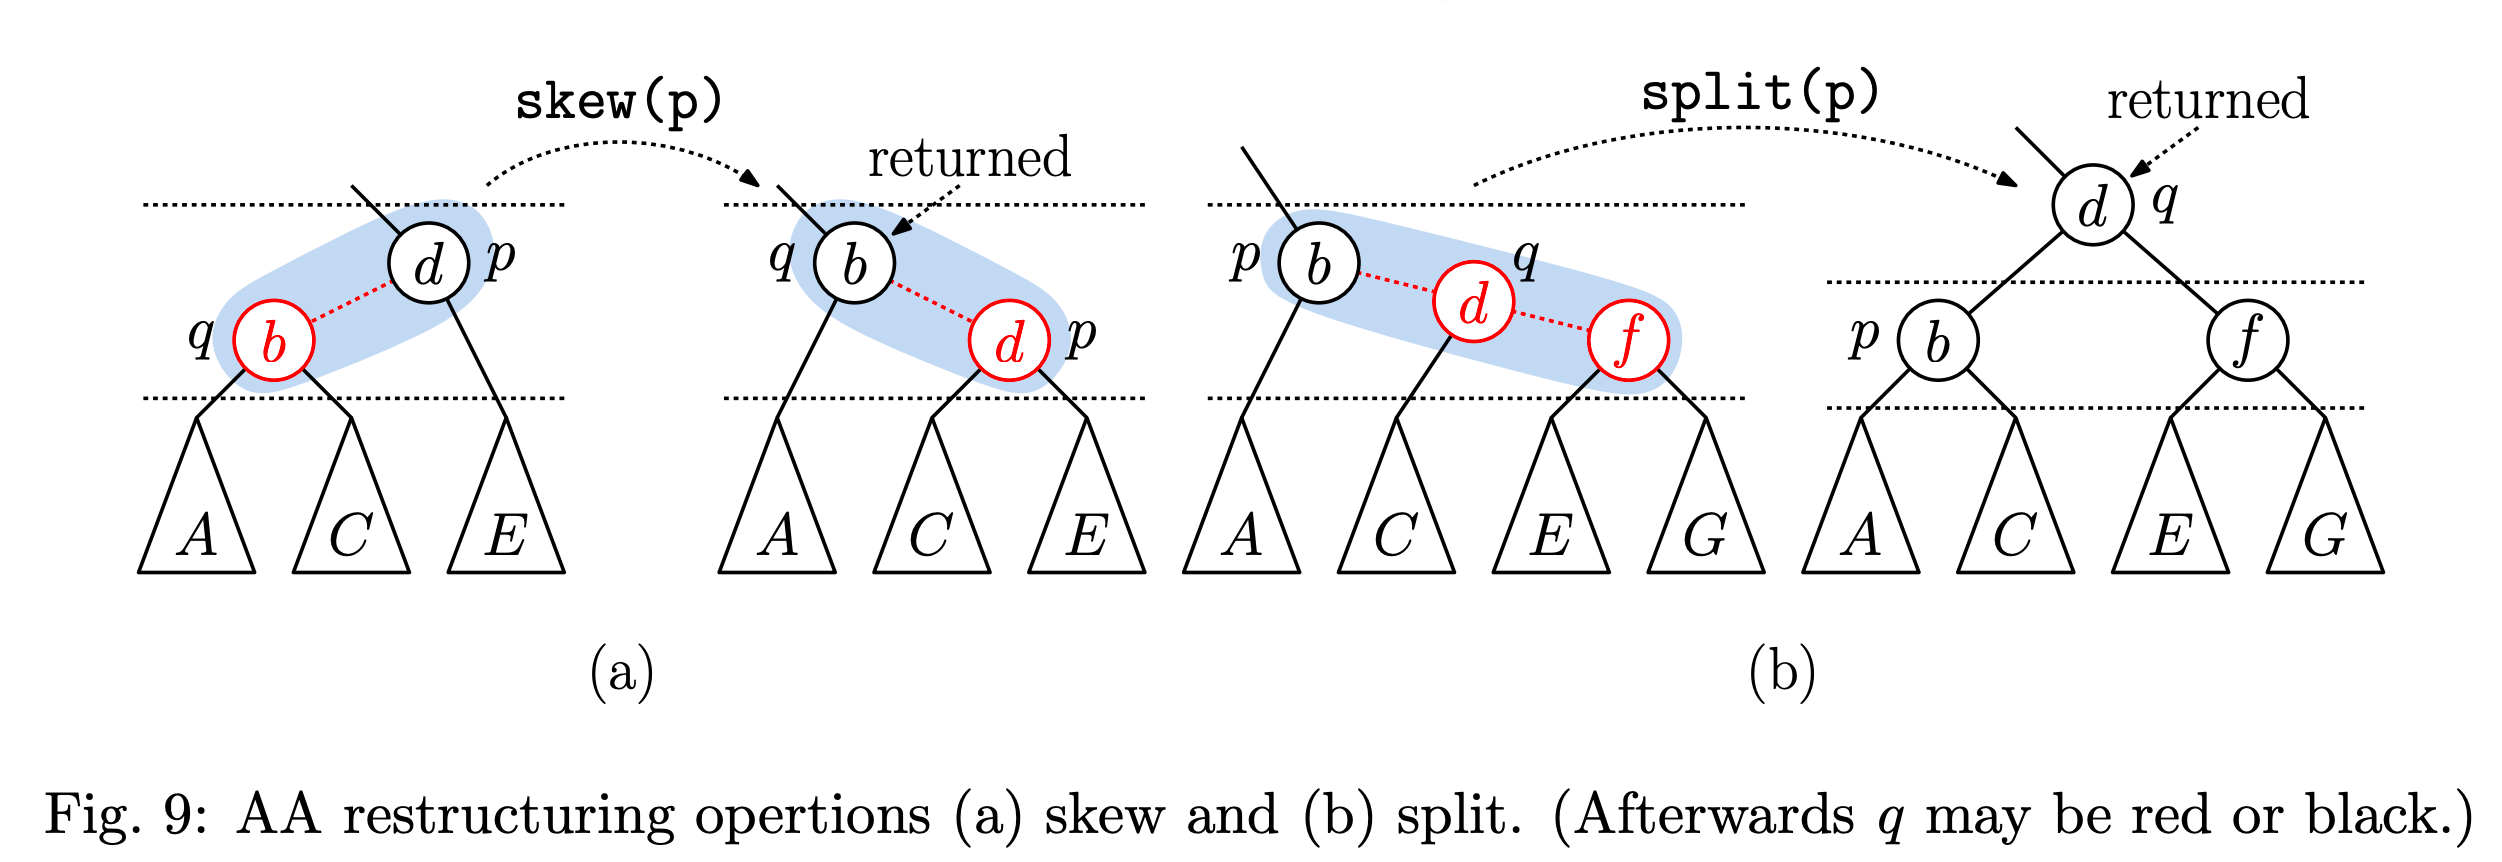
\includegraphics[scale=0.15]{AASkewSplit}
  \end{center}
  \textbf{Insertion: }insert node like in BST except treat it as a red node then work back up tree restructuring as we go.
  \begin{itemize}[noitemsep]
  \item If red node inserted as left child then perform skew(p) on parent
  \item If red node inserted as right child of red node, call split(p) on grandparent and then recurse up to fix any issues
  \end{itemize}
  \begin{lstlisting}
    AANode insert(Key x, Value v, AANode p) {
      if (p == nil) p = new AANode(x, v, 1, nil, nil)       //fell out so create new leaf
      else if (x < p.key) p.left = insert(x, v, p.left);
      else if (x > p.key) p .right = insert(x, v, p.right);
      else throw DuplicateKeyException;
      return split(skew(p));        //restructure (if not needed split and skew return unmodified tree)
    }
  \end{lstlisting}
  \begin{center}
  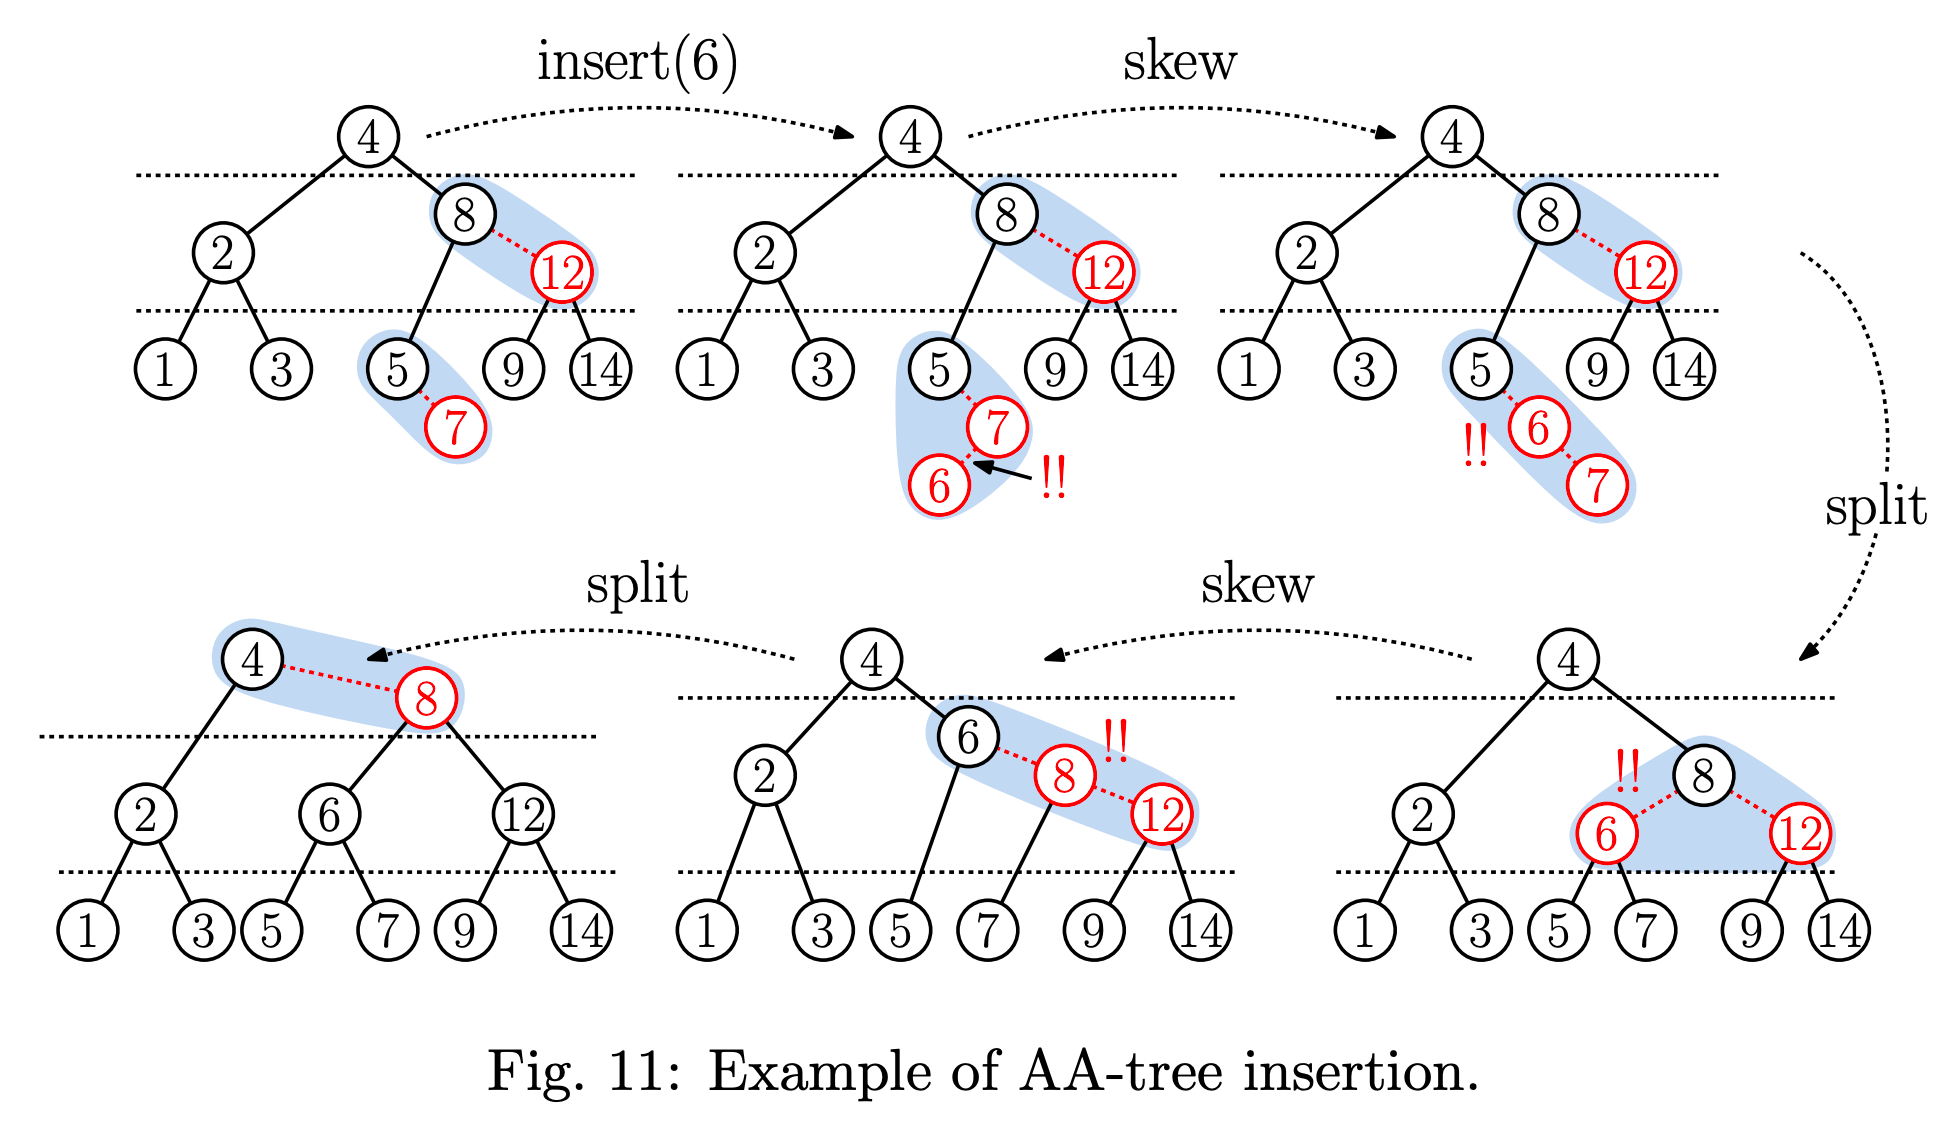
\includegraphics[scale=0.2]{InsertionAATree}
  \end{center}
  \textbf{Deletion: }Replace target node with inorder successor then delete leaf and retrace search path to restructure tree
  \begin{itemize}[noitemsep]
    \item use \textbf{updateLevel(p)} helper to update level of node p based on children (we need to update p.level to child.level which has been decreased)
    \begin{itemize}[noitemsep]
      \item since every node has at least 1 black node, ideal level for any node is 1 + min of its children 
      \item if p is updated and right child is red then we need to update p.right.level = p.level
    \end{itemize}
  \end{itemize}
  \begin{lstlisting}
    AANode updateLevel(AANode p) {
      int idealLevel = 1 + min(p.left.level, p.right.level);
      if (p.level > idealLevel) {
        p.level = idealLevel;
        if(p.right.level > idealLevel) p.right.level = idealLevel;  //is right child a red node?
      }
    } 
  \end{lstlisting}
  Use \textbf{fixupAfterDelete(p)} to make sure any red children are on the right
  \begin{itemize}[noitemsep]
  \item May need to call up to 3 skew operations (p, p.right, p.right.right) and then 2 splits (p and its right-right grandchild). The example below shows how there might be a 2 level gap between a parent and a child, which could end up necessitating 3 skew operations which then require 2 splits to fix
  \end{itemize}
  \begin{lstlisting}
    AANode fixupAfterDelete(AANode p) {
      p = updateLevel(p);
      p = skew(p);
      p.right = skew(p.right);
      p.right.right = skew(p.right.right);
      p = split(p);
      p.right = split(p.right);
      return p;
    }
  \end{lstlisting}
  \begin{center}
  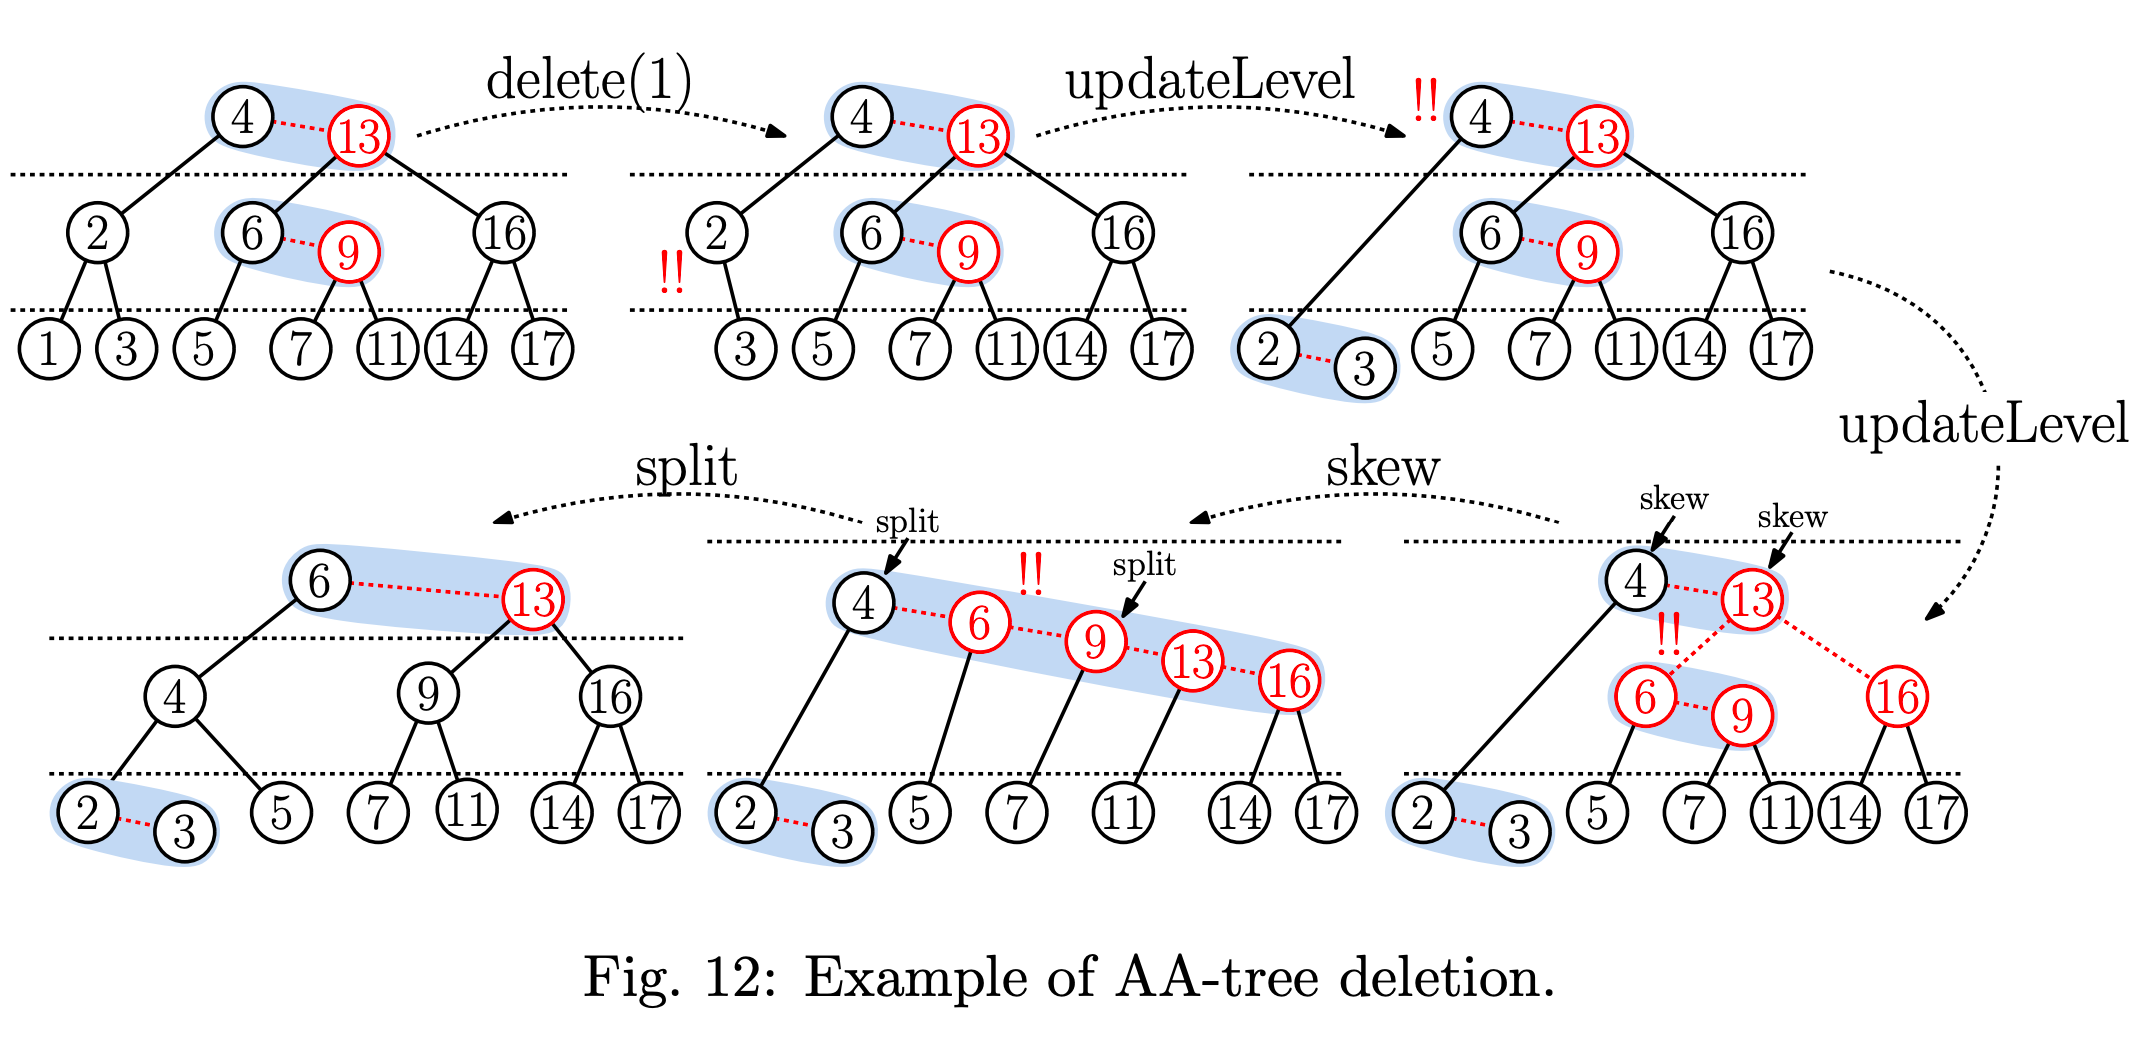
\includegraphics[scale=0.2]{DeletionAATree}
  \end{center}
  \begin{lstlisting}
    AANode delete(Key x, AANode p) {
      if (p == nil) throw KeyNotFoundException;
      else {
        if (x < p.key) p.left = delete(x, p.left);
        else if (x > p.key) p.right = delete(x, p.right);
        else {
          if (p.left == nil && p.right == nil) return nil;
          else if (p.left == nil) {           //no left child
            AANode r = inOrderSuccessor(p);
            p.copyContentsFrom(r);
            p.right = delete(r.key, p.right);
          } else {                            //no right child
            AANode r = inOrderPrdecessor(p);
            p.copyContentsFrom(r);
            p.left = delete(r.key, p.left);
          }
        }
        return fixupAfterDelete(p);
      }
    }
  \end{lstlisting}
  \newpage
  \section{Treaps and Skip Lists}
  \subsection{Treaps}
  Intuition is that if keys are inserted into BST in random order, then height will be $\approx$ O(log(n)). We can model this random order by using random priority numbers\\ \\
  \textbf{Insertion: }Insert node based on key value then assign it a random priority (p.priority) and then rotate the tree to balance it based on p.priority
  \begin{center}
  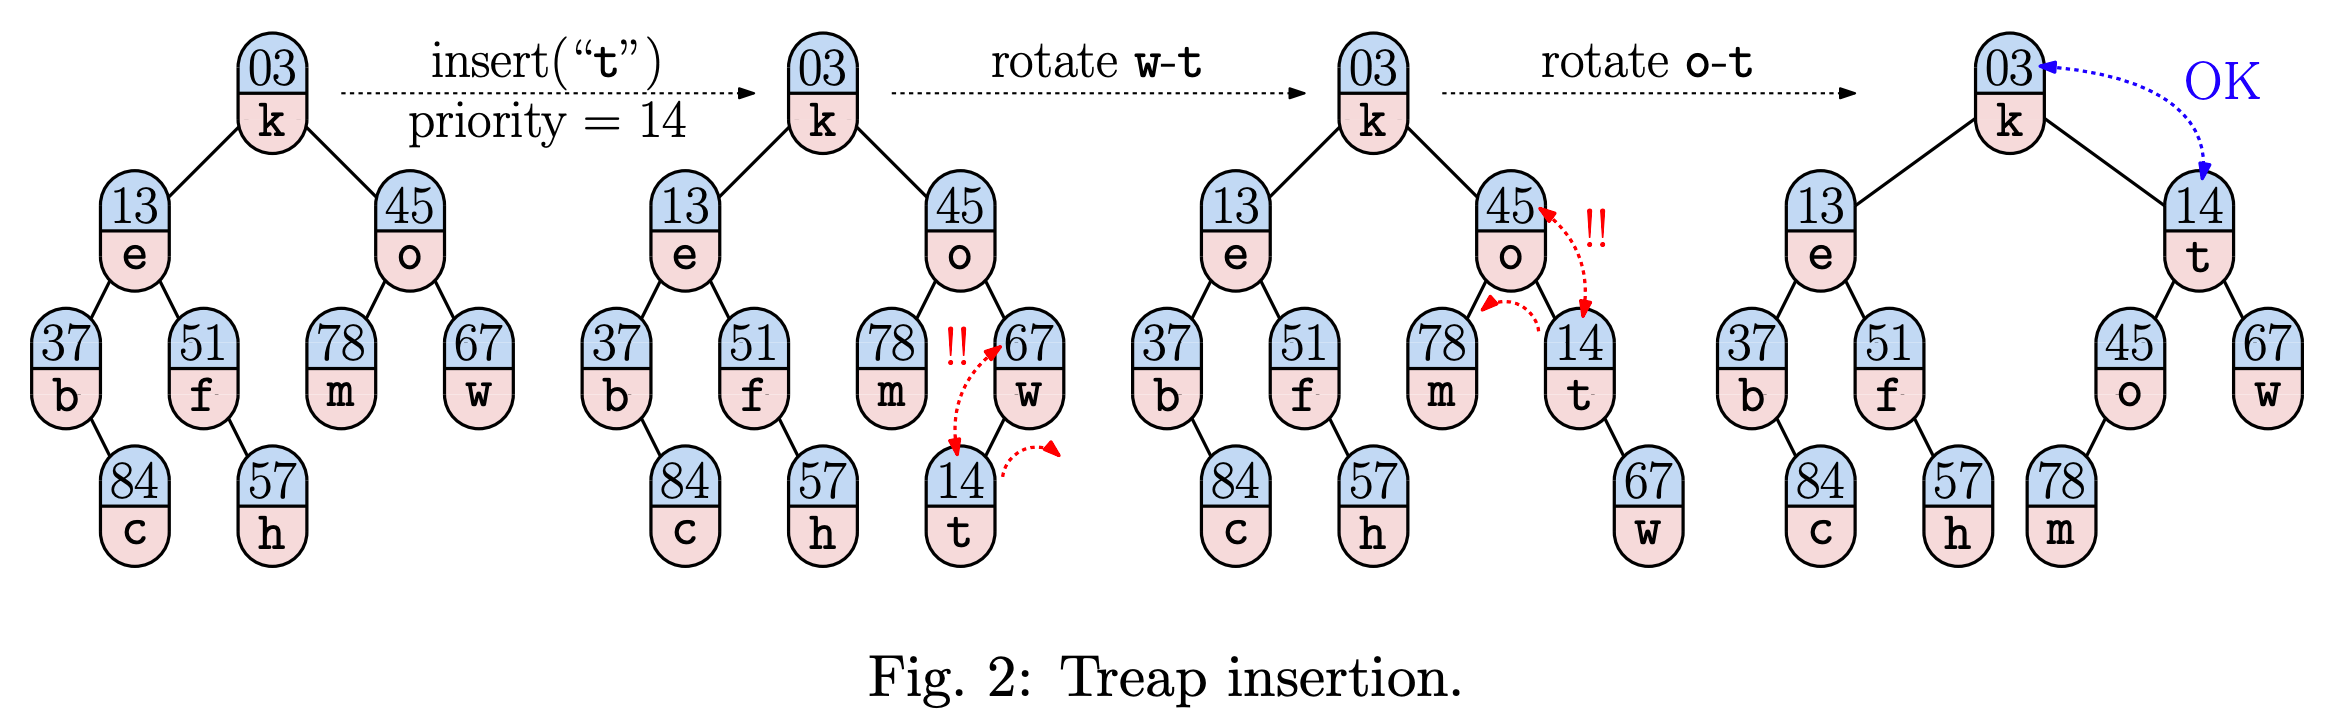
\includegraphics[scale=0.2]{TreapInsertion}
  \end{center}
  \textbf{Deletion: }3 cases
  \begin{itemize}[noitemsep]
  \item node is leaf just remove it
  \item node has 1 child then replace node with child
  \item node has 2 children then set its priority to $\infty$ and apply rotations to sift down to leaf and remove
  \end{itemize}
  \begin{center}
  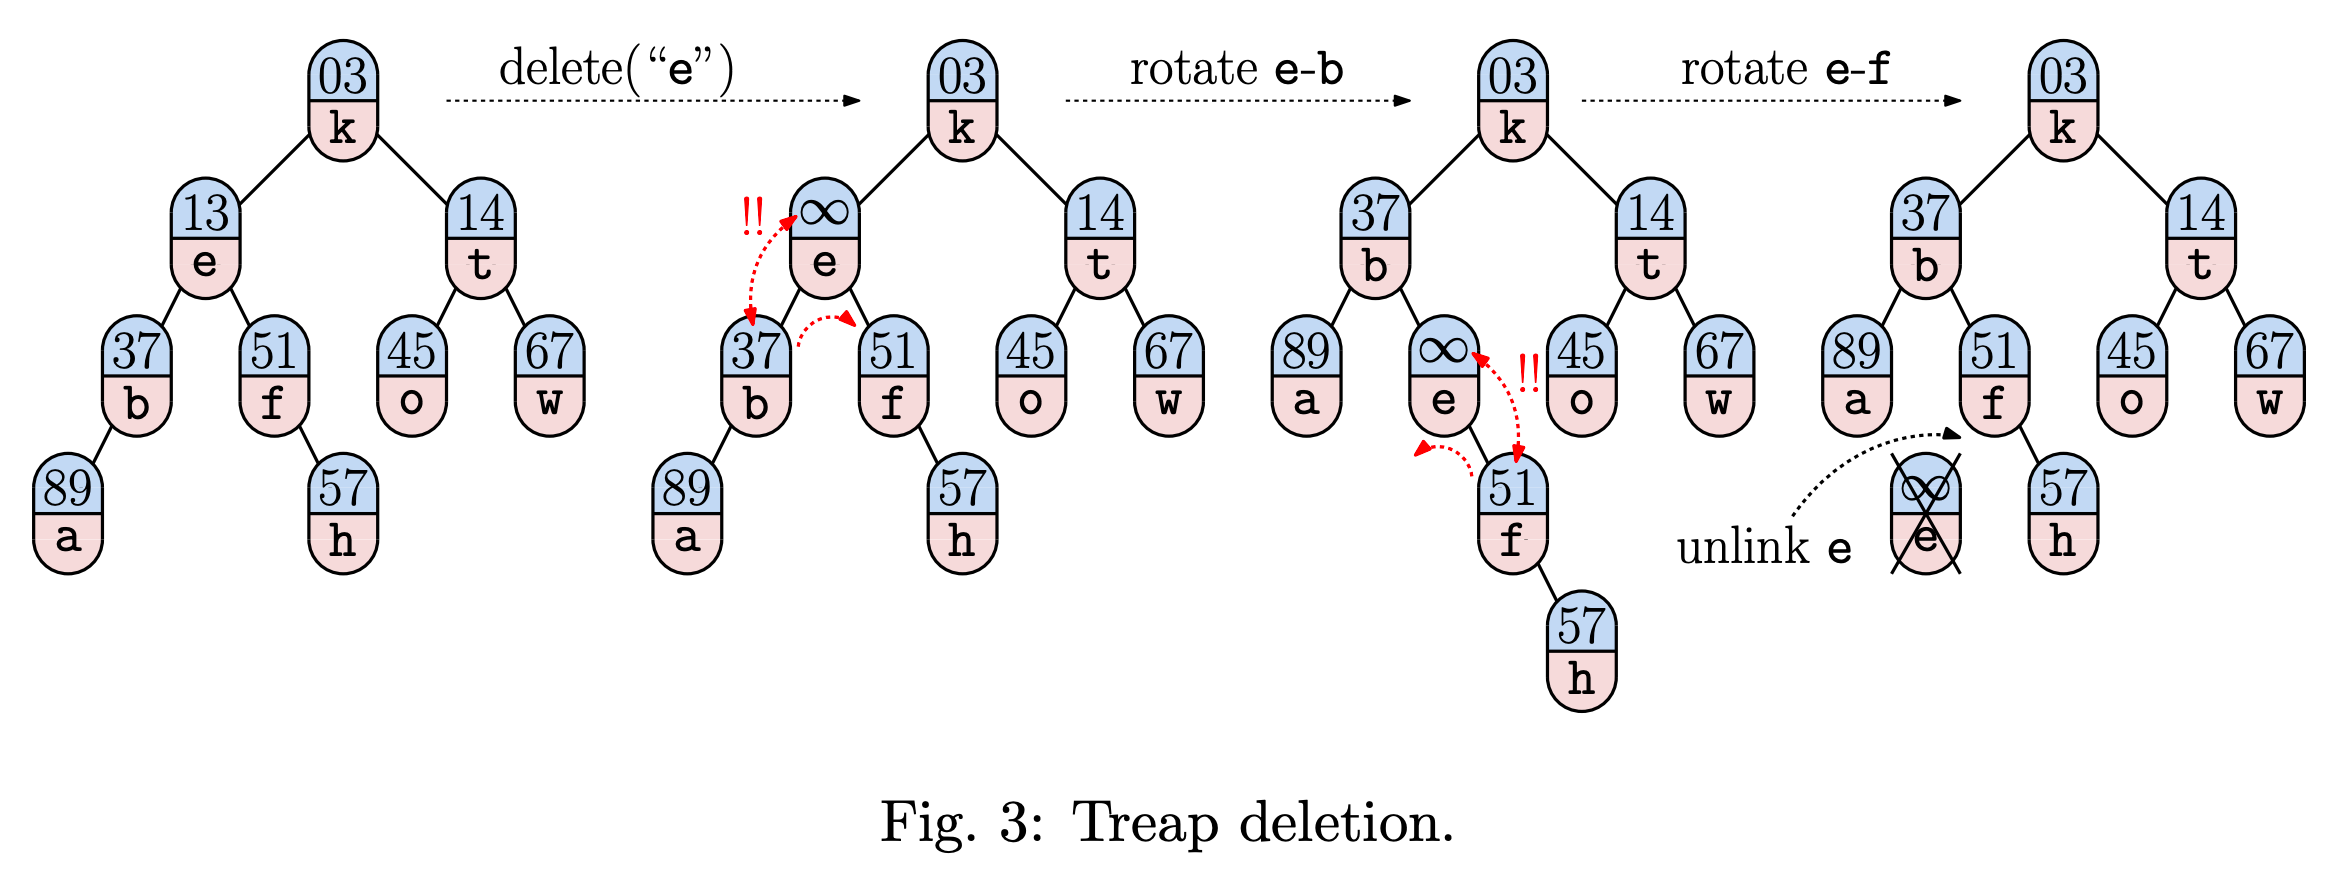
\includegraphics[scale=0.2]{TreapDeletion}
  \end{center}
  \subsection{Skip Lists}
  Intution is to skip multiple items at a time to speed up searching for linked list\\
  Skip Lists made up of multiple levels that are built from
  \begin{itemize}[noitemsep]
  \item Taking every other node in the linked list and extending it up to a new linked list with 1/2 as many nodes
  \item Repeat this extension with 1/2 as many terms until no more terms 
  \item Head and tail nodes are always lifted and tail has the key value $\infty$
  \item Height will be $\ceil[\big]{lg(n)}$ 
  \end{itemize}
  \textbf{Search: }start at highest level of head then scan linearly at level i until we are about to jump to a key value $>$ x then step down one level
  \begin{center}
  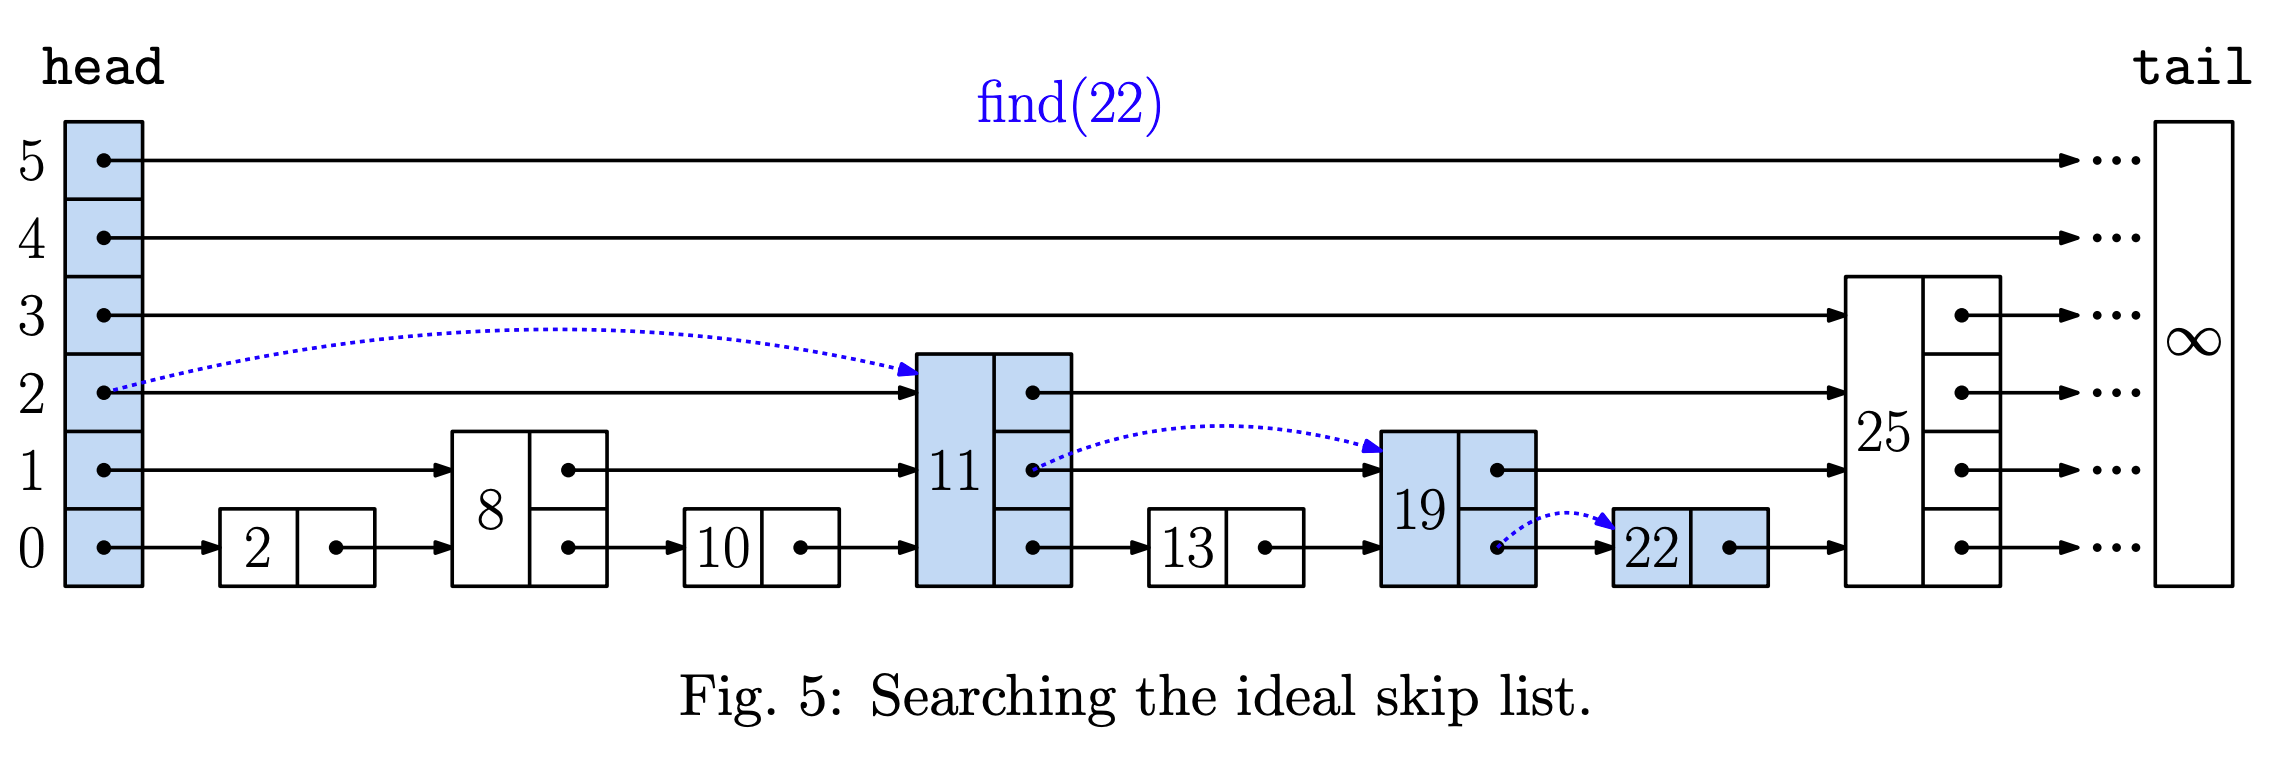
\includegraphics[scale=0.2]{SkipListSearch}
  \end{center}
  Issue with this deterministic skip list is that when we insert or remove a node, we need to change the heights of all subsequent nodes\\
  We can randomize the number of nodes per level by flipping a coin and only stopping at a level if tails occurs\\
  Now level k is expected to have about $\frac{n}{2^{k}}$ nodes meaning that the number of nodes at level $\ceil[\big]{lg(n)}$ is constant\\ \\
  \textbf{Space Analysis: }worst case every node has height log(n) so O(nlogn) total. Best each node has height 1 so O(n) total\\
  \textbf{Expected Case Space: }all n nodes contribute to level 0, n/2 contribute to level 1, n/4 to level 2, etc. so\
  \begin{center}
  $\sum_{i=0}^{h-1}\frac{n}{2^{i}} = n(2 - \frac{1}{2^{h}}) \leq 2n = O(n)$
  \end{center}
  \textbf{Search Expected Runtime: }for $0 \leq i \leq O(logn)$, let $E(i)$ represent the expected number of nodes visited in the skip list at the top i levels of the skip list\\
  Look at the path going backwards so it will either go up or stay on the current level and go left \\
  Whenever we arrive at some node of level i, the probability that it contributes to the next higher level is 1/2 and 1/2 to stay on same level. Counting the current node we just visited (+1) we have\\ \\
  $E(i) = 1 + \frac{1}{2}E(i-1) + \frac{1}{2}E(i) \rightarrow E(i) = 2 + E(i-1) = 2i$ by recurrence analysis and since i $\leq$ O(logn) then search is O(logn)\\ \\
  \textbf{Insertion: }search for x to find its immediate predecessors at each level then create node x and flip a coin until tails. Letting k denote the number of tosses made, height = min of k + 1 and height of list then link the k+1 lowest predecssors \\ \\
  \textbf{Deletion: }find the node and keep track of all predecessors at various level of list then unlink the target node at each level (like in standard linked list removal) \\ \\
  \textbf{Implementation Notes: }skip-list nodes have variable size, containing the key-value pair, variable-sized array of next pointers (p.next[i] points to the next node at level i). Also has 2 sentinel nodes (head and tail where tail.key is $\infty$ to stop search)\\
  \newpage
  \section{Splay Trees}
  Self adjusting tree that dynamically adjusts its structure according to a dynamically changing set of access probabilities
  \begin{itemize}[noitemsep]
  \item nodes that are accessed more frequently are closer to the root
  \item Binary Search Tree that uses rotations to maintain structure but doesn't need to store balance information
  \item Whenever a deep node is accessed, the tree will restructure itself so tree is more balanced 
  \item $\Omega(n)$ worst operation but amortized O(logn) \\
  \end{itemize}
  \textbf{T.splay(x): }searches for key x in a tree T and reorganizes T while rotating x up to the root. If x not found, then use the last node before falling out the tree which will be the inorder predecessor or successor.
  \begin{itemize}[noitemsep]
  \item simply rotating the target node up doesn't work because it can leave the tree skewed/unbalanced
  \item instead take 2 nodes at a time and rotate both
  \end{itemize}
  For node p let parent be q and grandparent be r then
  \begin{itemize}[noitemsep]
  \item Zig-zig: if p and q are both right children or left children, apply rotation at r then q to bring p to the top
  \item Zig-zag: if p and q are left-right or right-left children, apply rotation to q then r to bring p to top 
  \item Zig: if p is the child of the root, rotate root of T and make p the new root
  \item if p is the root of T, we are done
  \end{itemize}
  \begin{center}
  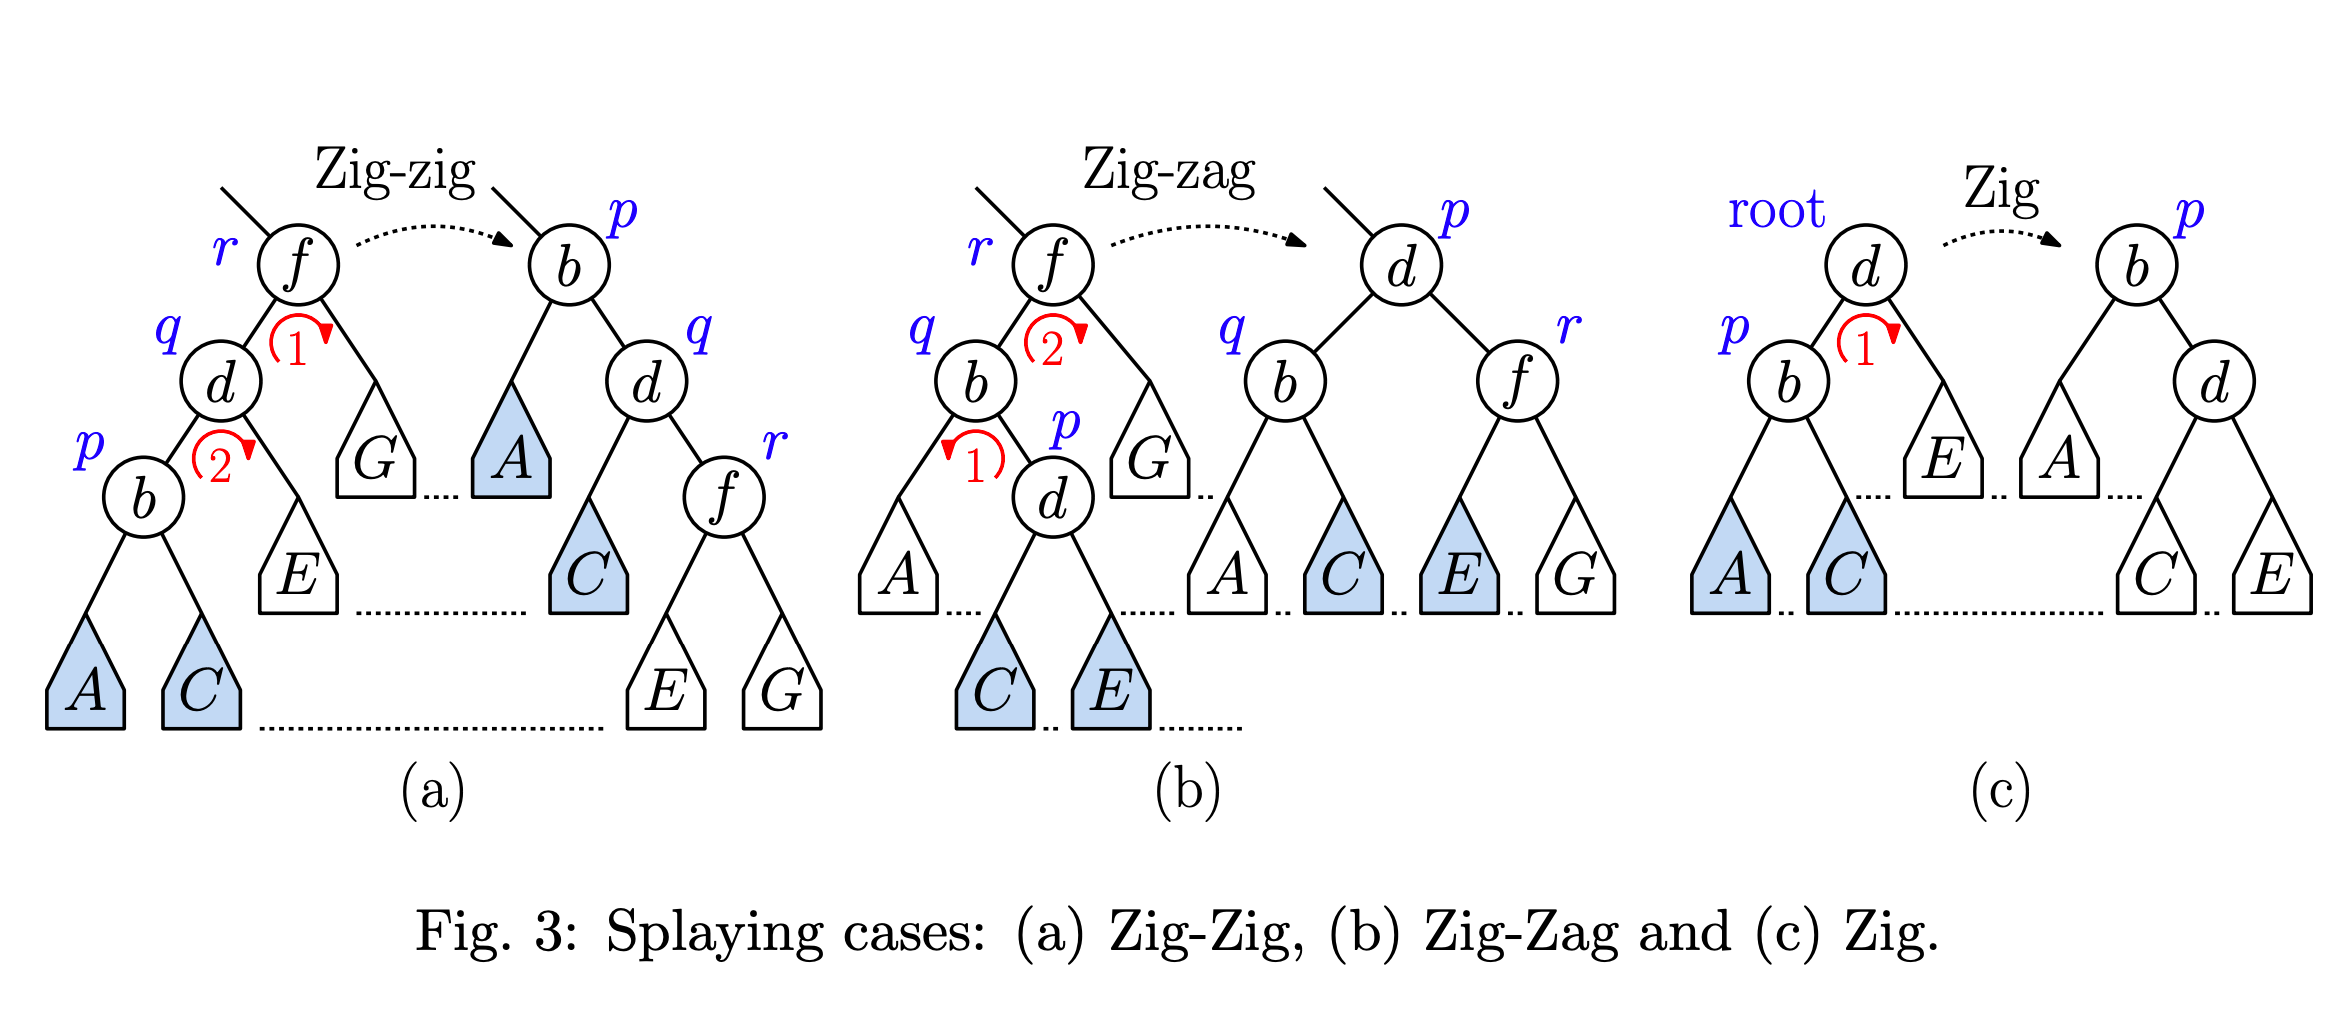
\includegraphics[scale=0.20]{SplayTreeZig}
  \end{center}
  Everytime zig-zig or zig-zag is called, the subtree is raised up 1 level so for a long path, these rotations will reduce its height by 1/2\\ \\
  \textbf{Find: }invoke T.splay(x) which transports x to the root. If root.val != x then throw an error\\ \\
  \textbf{Insert(x, v): }invoke T.splay(x). Let current root = y. Either
  \begin{itemize}[noitemsep]
  \item y $<$ x then all keys in R subtree $>$ x so create a new root (x,v) and add y to L and add R to new root
  \item y $>$ x then all keys in L $<$ x so create a new root (x,v) and add y to R and add L to new root
  \end{itemize}
  \begin{center}
  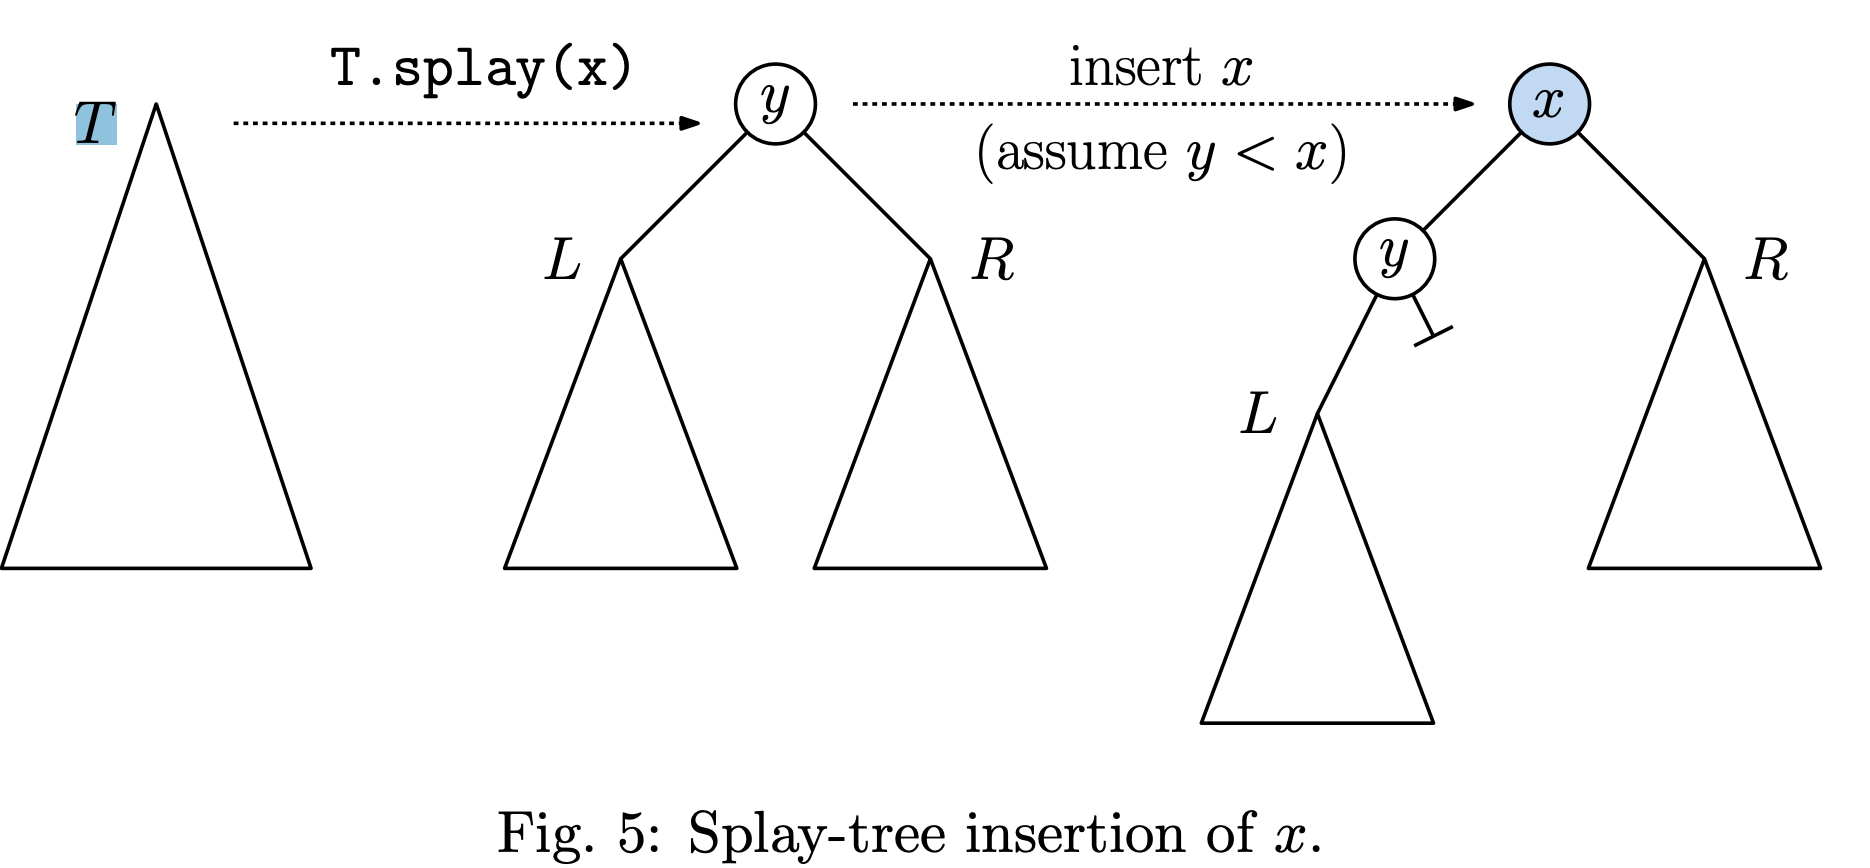
\includegraphics[scale=0.15]{SplayInsert}
  \end{center}
  \textbf{Delete: }invoke T.splay(x) then if root != x throw error. Else 
  \begin{itemize}[noitemsep]
  \item if L is empty return R
  \item if R is empty return L 
  \item Otherwise let R' = R.splay(x). This will find the inorder successor y. Since y will have no left subtree (all values in R are $>$ x), make y the new root and link L
  \end{itemize}
  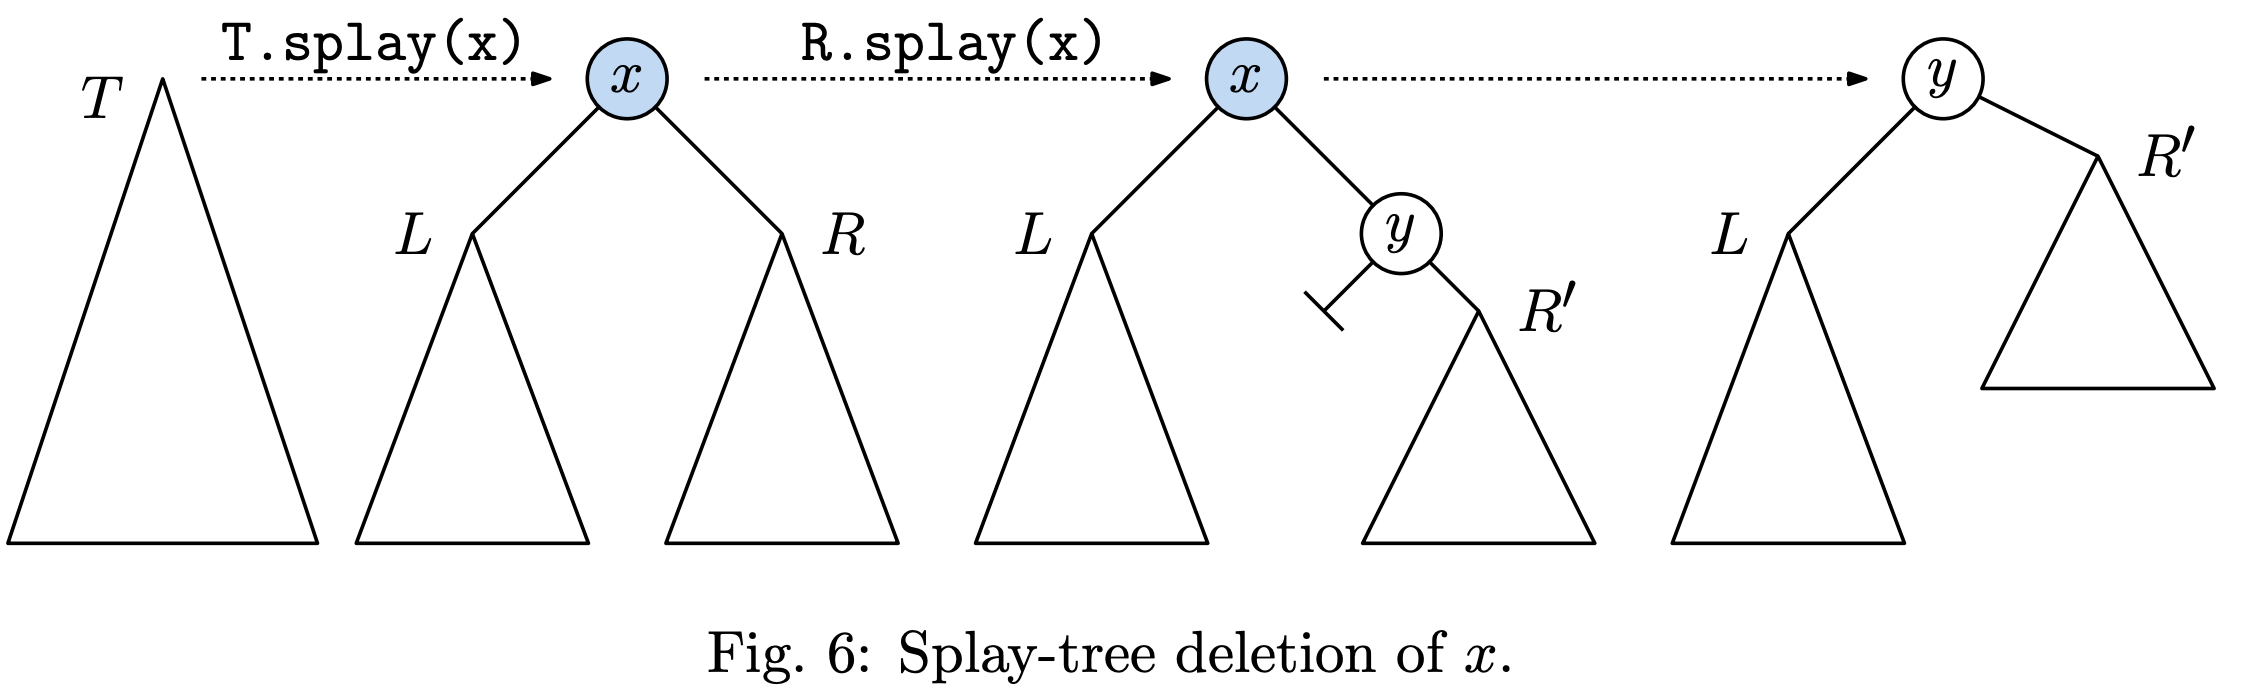
\includegraphics[width=\textwidth]{SplayDelete}
  \newpage
  \section{B-Trees}
  J-ary multiway search trees where each node stores reference to j subtrees $T_{1}, T_{2}, ..., T_{j}$ and has j-1 keys $a_{1} < a_{2} < a_{j-1}$ such that each $T_{i}$ subtree stores nodes whos keys are $> a_{i-1}$ and $< a_{i}$\\ 
  Achieves balance by constraining width of each node \\
  For any int m $\geq$ 3, B-tree of order m is a multiway search tree if: 
  \begin{itemize}[noitemsep]
  \item root is leaf or has $2 \leq x \leq m$ children
  \item each node except root has between $\ceil[\Big]{\frac{m}{2}}$ and m children which can be null
  \begin{itemize}[noitemsep]
    \item node with j children has j-1 keys
  \end{itemize}
  \item All leaves are on the same level of the tree \\
  \end{itemize}
  \textbf{Height Analysis: }as B-Trees grow wider, the height decreases\\
  \textbf{Theorem: }B-Tree of order m with n keys has height of at most $(lgn)/\gamma$ where $\gamma$ = lg(m/2)\\
  \textbf{Proof: }assume m is even and let N(h) = number of nodes in skinniest possible order-m B tree of height h\\
  \indent Root has $\geq$ 2 children that have $\geq$ m/2 children \\
  \indent \indent therefore 2 nodes at depth 1\\
  \indent \indent $2(m/2)$ nodes at depth 2\\
  \indent \indent $2(m/2)^{2}$ nodes at depth 3\\
  \indent \indent $2(m/2)^{k-1}$ nodes at depth k\\
  \indent So $N(h) = \sum_{i=1}^{h}2(\frac{m}{2})^{i-1}$\\
  \indent let c = m/2\\
  \indent $N(h) = \frac{2(c^{h}-1)}{(c-1)} \approx \frac{2c^{h}}{c} = 2c^{h-1} = 2(\frac{m}{2})^{h-1}$\\
  \indent Each node has $\geq \frac{m}{2}-1$ keys $\approx \frac{m}{2}$\\
  \indent $n \geq N(h) \geq 2(\frac{m}{2})^{h} \rightarrow h \leq \frac{lgn}{lg\frac{m}{2}}$\\ \\
  \textbf{Node Structure: }since B-Tree nodes can hold a variable number of items, every node is allocated max possible size but not all of the space allocated may be used
  \begin{lstlisting}
    final int M = m;    \\order of B-tree
    class BTreeNode {
      int nChildren;
      BTreeNode child[M];
      Key key[M-1];
      Value value[M-1]; 
    }
  \end{lstlisting}
  \textbf{Searching: }When arriving at an interval node, search through keys
  \begin{itemize}[noitemsep]
  \item if x is found then return the corresponding value
  \item Else determine index i such that $a_{i-1} < x < a_{i}$ note that $(a_{0} = -\infty, a_{j} = \infty)$
  \item Then recurse into subtree $T_{i}$\\
  \end{itemize}
  Insertion and Deletion require some restructuring methods (rotation, splitting, and merging)\\
  \textbf{Rotation (Adoption): }Node can have between $\ceil[\Big]{m/2}$ and $m$ children, and one less keys. Insertion and deletion might make a node have too many or too few nodes so we fix this imbalance by moving a child into or from one of its siblings and rotate a key from parent, assuming can give a child\\
  \begin{center}
  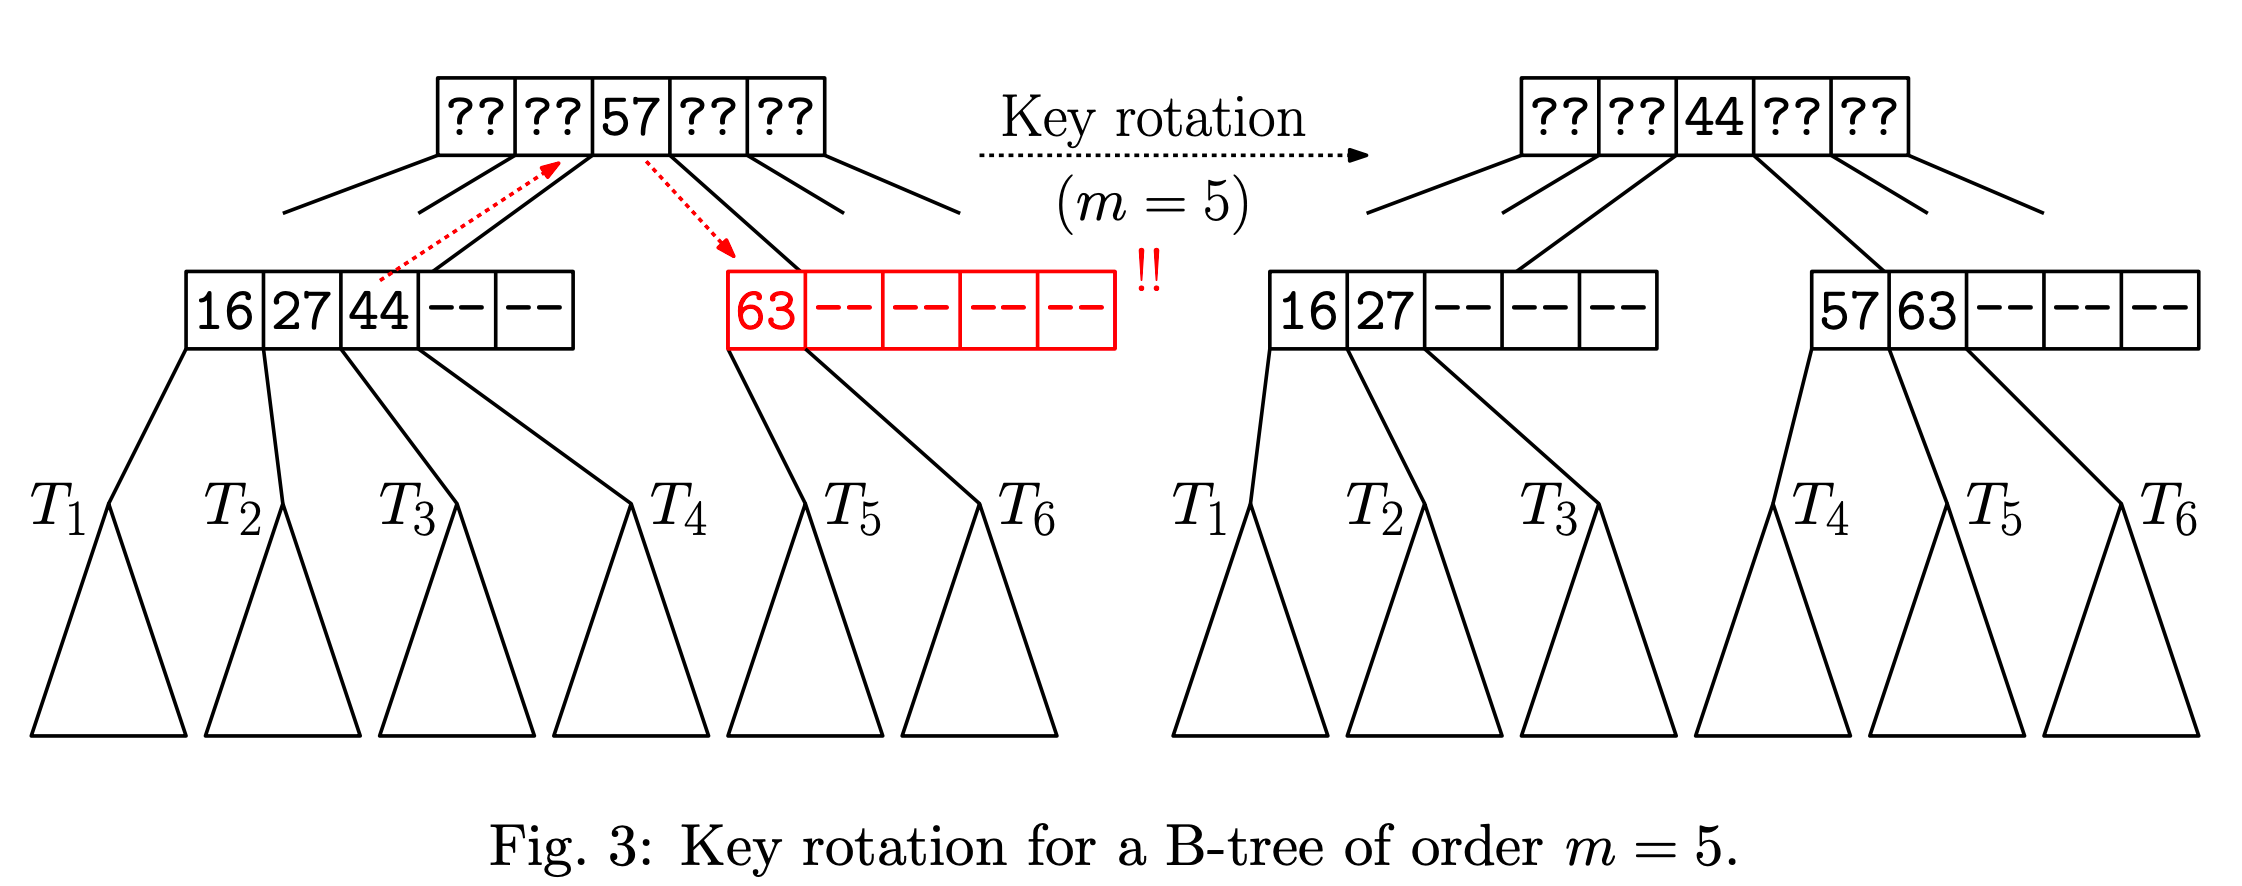
\includegraphics[scale=0.10]{BTreeRotations}
  \end{center}
  \textbf{Node Splitting: }node has 1 too many children (m + 1 children and m keys) and key rotation is not available so split node into 2 nodes, one with $m' = \ceil[\Big]{m/2}$ children and the other with $m''= m + 1 - \ceil[\Big]{m/2}$ children\\
  Since $(m' - 1) + (m'' - 1) = m - 1$, we have one extra key that is doesn't fit into L and R subchildren so it is promoted to parent and then handled up there
  \begin{center}
  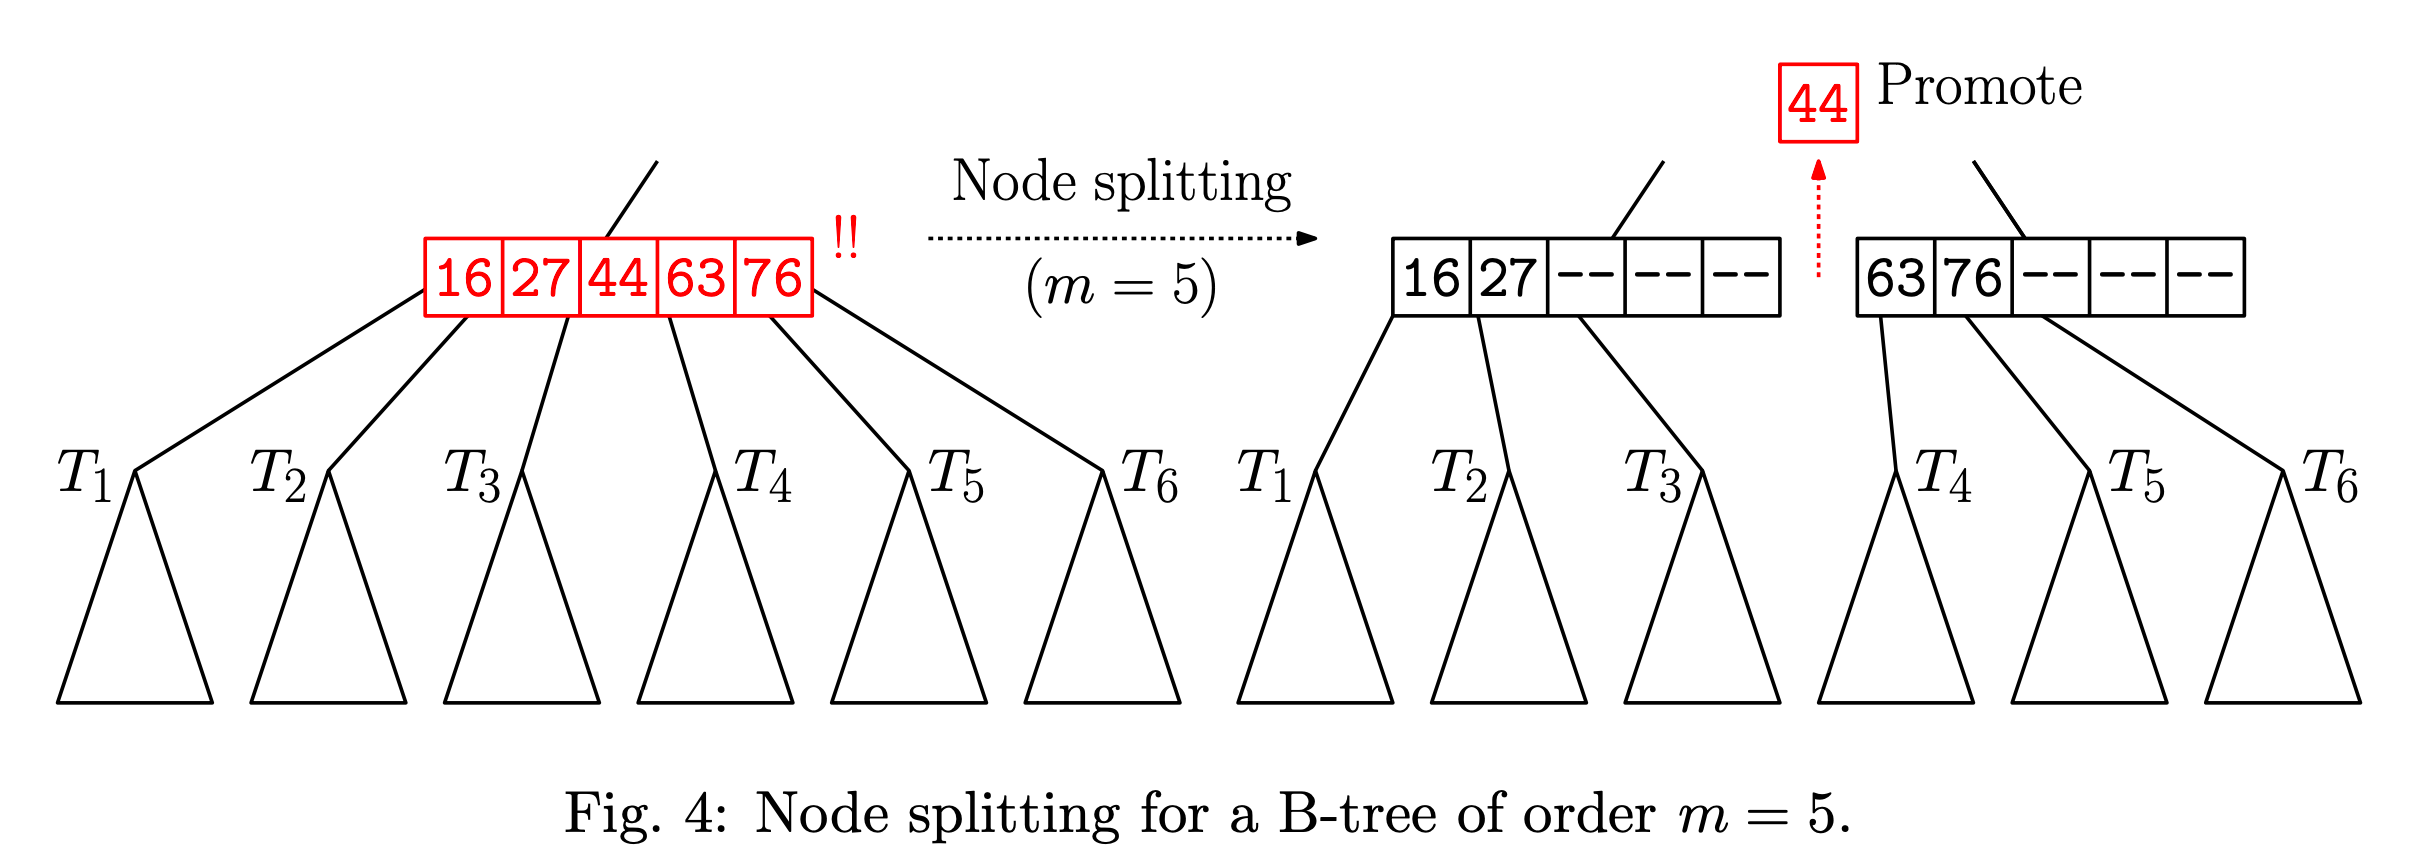
\includegraphics[scale=0.15]{BTreeNodeSplitting}
  \end{center}
  Proof for Node Splitting:
  \begin{itemize}[noitemsep]
  \item If m is even then $\frac{m}{2} \leq m + 1 - \frac{m}{2} = \frac{m}{2} + 1 \leq m$
  \item If m is odd then $\frac{m+1}{2} \leq m + 1 - \frac{m+1}{2} = \frac{m+1}{2} \leq m$ \\
  \end{itemize}
  \textbf{Node Merging: }Node might have 1 too few children ($\ceil{m/2} - 1$ nodes and one less keys) after deletion. If key rotation isn't available, then we know that the sibling must have the minimum number of children $(\ceil[\Big]{m/2})$. Now merge node with the sibling into a node with $m' = (\ceil[\Big]{m/2} - 1) + \ceil[\Big]{m/2} = 2\ceil[\Big]{m/2} - 1$ children\\
  Note that $\ceil{m/2} - 2 + \ceil{m/2} - 1 = m' - 2$ which is one too few keys so we demote the appropriate key from the parent's node to get desired number of keys. \\
  Since the parent lost a key and a node, recurse up to parent\\ \\
  Proof for Node Merging: For all $m \geq 2$, $\ceil{m/2} \leq 2\ceil{m/2} - 1 \leq m$
  \begin{itemize}[noitemsep]
  \item If m is even then $\frac{m}{2} \leq m - 1 \leq m$
  \item If m is odd then $\frac{m+1}{2} \leq m \leq m$
  \end{itemize}
  \begin{center}
  \includegraphics[scale=0.15]{BtreeNodeMerge}
  \end{center}
  \textbf{Insertion: }creating nodes is an expensive operation so try to rotate whenever possible. Search for key x and if
  \begin{itemize}[noitemsep]
  \item found thrown an exception
  \item leaf is not at full capacity (fewer than m-1 keys) then we insert key and done
    \begin{itemize}[noitemsep]
      \item may involve sliding around but can ignore the cost since m is constant
    \end{itemize}
  \item otherwise node overflows and check if either sibling is less than full. If so then perform a rotation else perform node split. 
  \end{itemize}
  \begin{center}
  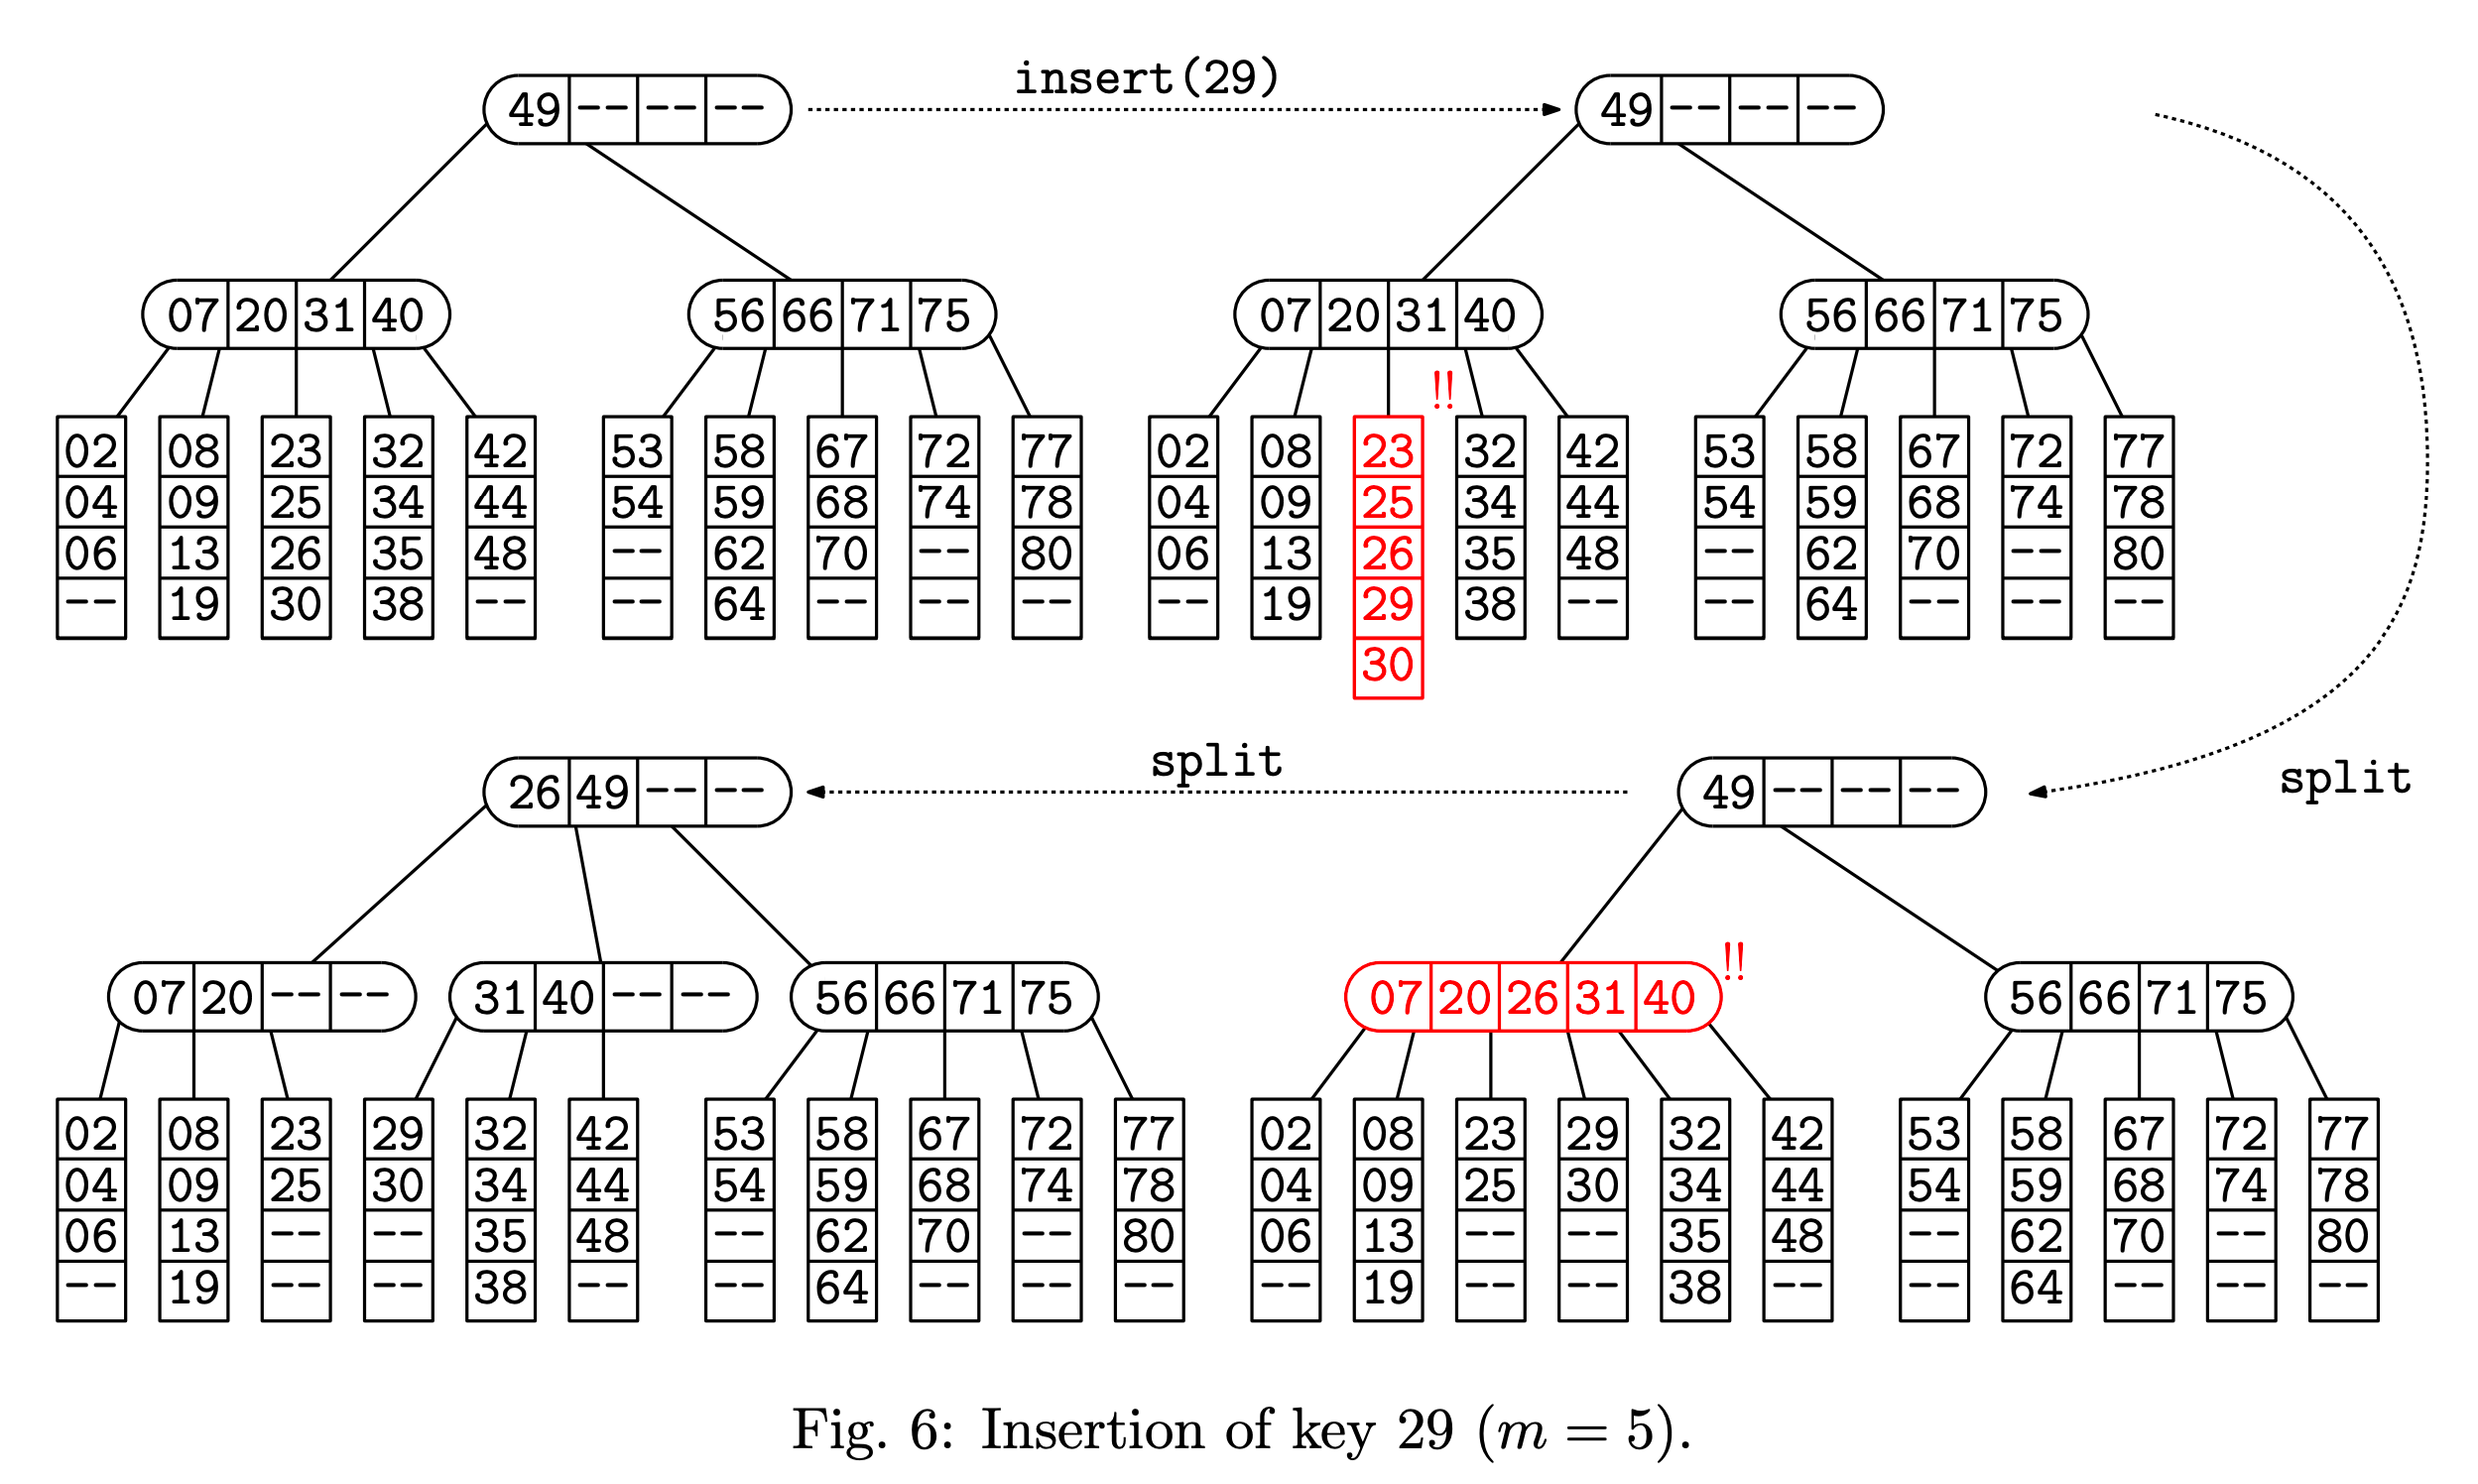
\includegraphics[scale=0.15]{BTreeInsertion}
  \end{center}
  \textbf{Deletion: }Search for the node to be deleted. Need to find replacement so take largest key in left child or smallest key in right child and move this key up to fill the hole
  \begin{itemize}[noitemsep]
  \item if left node has $\geq \ceil{m/2} - 1$ keys we are done
  \item else node will underflow so key rotate if possible else use node merge and recurse in parent
  \end{itemize}
  \begin{center}
  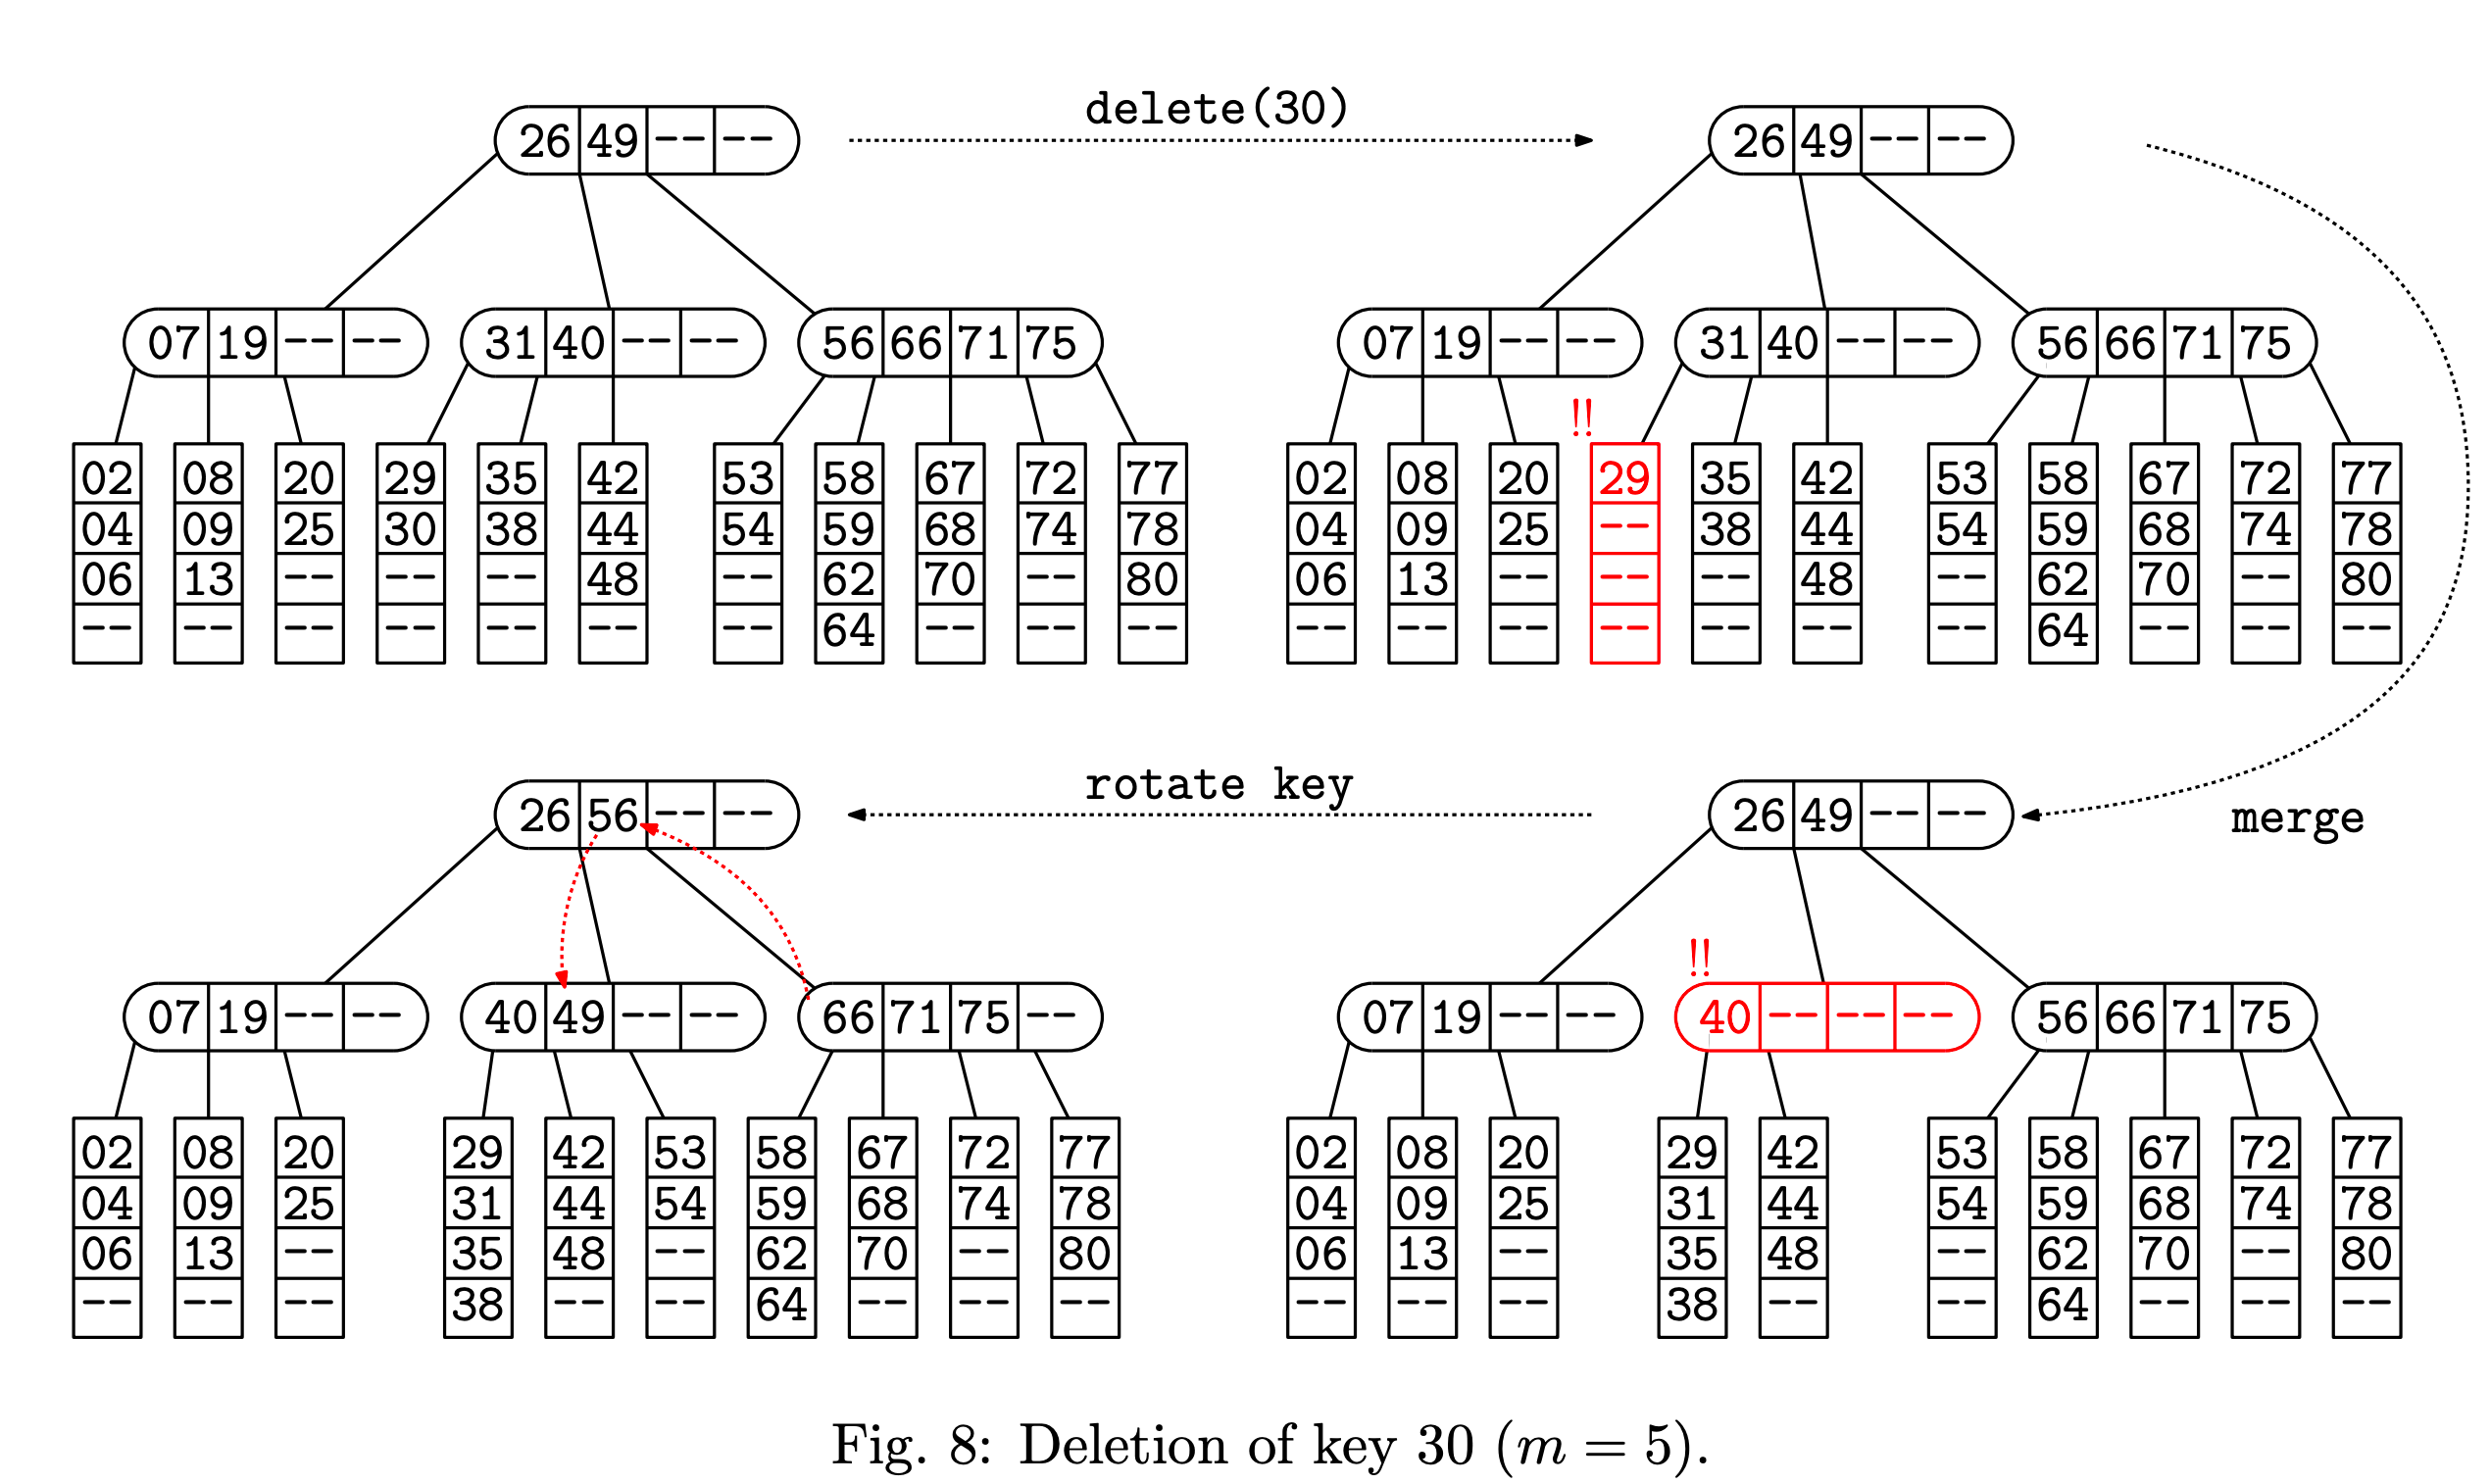
\includegraphics[scale=0.15]{BTreeDeletion}
  \end{center}
  \textbf{B+ Trees: }internal nodes only store keys (not values)\\
  Keys are used solely for locating leaf node containing actual data so it's not necessary that every key in internal node to correspond to a key-value pair\\
  Each leaf node has a next-leaf pointer, which pointers to the next leaf in sorted order \\
  Storing only keys in internal nodes save space and allows increased tree fan out $\rightarrow$ lowers height of tree\\
  Internal nodes are an index to locate actual data which resides at the leaf level\\
  Now internal nodes with keys $a_{1}, ..., a_{j-1}$, subtree $T_{j}$ has keys x such that $a_{i-1} < x \leq a_{i}$\\
  Next leaf enables efficient range reporting queries where we can list keys in range $[x_{min}, x_{max}]$\\
  \indent so we now find the leaf node $x_{min}$ and follow next leaf links until we reach $x_{max}$\\
  \newpage
  \section{Hashing}
  Supports O(1) dictionary operations but cannot perform search operations like range queries (finding keys x such that $x_{1} \leq x \leq x_{2}$) or nearest-neighbor queries (find key closest to a given key x)\\
  Given a table of size m $>$ n and a hash function h(x), we use h(x) to map a key to a random index $[0...m-1]$ \\
  Possible issue of collisions where 2 keys land in the same index after hashing\\ \\
  Good hash function:
  \begin{itemize}[noitemsep]
  \item Efficiently computable
  \item Produces few collisions
    \begin{itemize}[noitemsep]
      \item function on every bit of key 
      \item scatters naturally occuring clusters of keys \\
    \end{itemize}
  \end{itemize}
  Types of hasing:
  \begin{itemize}[noitemsep]
    \item \textbf{Division Hashing: }$h(x) = x \mod m$
    \begin{itemize}[noitemsep]
      \item Fails 2nd rule (issue with clusters)
    \end{itemize}
  \item \textbf{Multiplicative Hashing: }$h(x) = (ax) \mod m$
  \begin{itemize}
    \item Where a is a large prime number
  \end{itemize}
\item \textbf{Linear Hashing: }$h(x) = (ax + b) \mod m$
  \begin{itemize}
      \item Enhances Multiplicative hashing with added constant
  \end{itemize}
\item \textbf{Polynomial Hashing: }$h(x_{0}, ..., x_{n}) = (\sum_{i=0}^{k-1}c_{i}p^{i}) \mod m$
    \begin{itemize}
      \item Useful for keys that have a sequence of objects (strings or coordinates)
      \item Can use Horner's Rule to make summation faster $c_{0} + c_{1}p + c_{2}p^{2} + c_{3}p^{3} = ((c_{3}p + c_{2})p + c_{1})p + c_{0}$ \\
    \end{itemize}
  \end{itemize}
  \textbf{Universal Hashing: }hash function is selected from large class of functions so probability of collision between 2 fixed keys is about 1/m\\
  Consider a large prime $p$ and two random integers $a \in \{1, 2, ..., p-1\}$ and $b \in \{0, 1, ..., p-1\}$ \\
  Use a linear has function $h_{a,b}(x) = ((ax + b) \mod p \mod m$. As a and b vary, they will define a family of functions.\\ \\
  \textbf{Theorem: }Let $H_{p}$ denote the class of hash functions that arise from all possible combos of a and b. If we consider any two integers x and y such that $0 \leq y < x < p$ then the probability $h_{a,b}(y) = h_{a,b}(x)$ is 1/m
  \subsection{Handling Collisions}
  \textbf{Separate Chaining: }have each index be a linked list and store collisions by adding to these linked lists.
    \begin{itemize}[noitemsep]
    \item We define the load factor $\lambda = n/m$ and expect each list to have about $\lambda$ elements
    \item If we are successful in finding the desired element, it'll take about $1 + \frac{\lambda}{2}$ (about halfway). Otherwise failure will take $1 + \lambda$. Additional 1 is for null checks
    \item Insertion and deletion will take about constant time so all dictionary operations will take $O(1 + \lambda)$
    \item Drawback of we need to use additional storage to store pointers to linked lists
    \end{itemize}
  Controlling Load Factor and Rehashing: we want to maintain a few invariants
  \begin{center} 
    $0 < \lambda_{min} < \lambda_{max} < 1$ \quad $\lambda_{min} \leq \lambda \leq \lambda_{max}$ \quad $n \leq \lambda_{max}m$ \quad $m \leq n/\lambda_{min}$
  \end{center}
  We don't want too large of a table or too small of a table so the optimal load factor is $\lambda_{0} = (\lambda_{max} + \lambda_{min}) / 2$\\
  If load factor is too big ($n > lambda_{max}m$) or too small ($n < \lambda_{min}m$) then we rehash with a larger table
  \begin{itemize}
    \item Allocate a table of size $m' = \ceil{n/\lambda_{0}}$
    \item generate new hash function $h'$ using new table size
    \item Insert every entry from old table to new table using new hash function
    \item remove old table
    \item New load factor ($n/m'$) $\approx \lambda_{0}$ so we have restored optimal load factor
  \end{itemize}
  Amortized cost of rehashing is still good since we only rehash every so often \\ \\
  Open Addressing: To know which table entries have values and which are empty we store a special value \textit{empty}. Now whenever we insert an element and its hashed index is already occupied we probe around nearby entries until we find an empty slot. The secondary search involves a function $f$ so now the probe sequence is
  \begin{center}
    $(h(x) + f(1)) mod m, (h(x) + f(2)) mod m, ...$
  \end{center}
  \newpage
  Linear Probing: probe function is $f(i) = i$ and we search sequential locations until we find an empty slot
  \begin{itemize}[noitemsep]
    \item good for low load ($<75\%$)factor. As load factor approaches 1, becomes very bad
    \item Issue with secondary clustering (when keys has to different locations but collision-resolution results in new collisions)
    \item Successful search expected cost: $(\frac{1}{2}(1 + \frac{1}{1 - \lambda}))$ \quad Unsuccessful serach expected cost: $(\frac{1}{2}(1 + (\frac{1}{1 - \lambda})^{2}))$ \\
  \end{itemize}
  Quadratic Probing: Avoids secondary clustering by using a nonlinear probing function, scattering subsequent probes. Example Code:
  \begin{lstlisting}
    Value find(Key x) {
      int c = h(x);
      int i = 0;
      while ((table[c].key != empty) && (table[c].key != x)){
        c += 2*(++i) - 1;
        c = c \% m
      }
      return table[c].value;
    }
  \end{lstlisting}
  Quadratic Probing has a potential issue of skipping potential slots due to growth factor. However if m is prime, we can guarantee that $\ceil{m/2}$ probe sequences are distinct. Proof:\\
  Contradiction: assume $0 \leq i < j \leq \ceil{m/2}$ then \\
  $h(x) + i^{2} \equiv h(y) + j^{2} \iff i^{2} \equiv j^{2} \equiv i^{2} - j^{2} \equiv 0 \iff (i-j)(i+j) \equiv 0 mod m$ but its impossible since m is prime\\
  Other cool properties:
  \begin{itemize}[noitemsep]
    \item if $m = 4k + 3$ and is prime, then quadratic probe will work for all table entries before repeating
    \item if m is a power of 2 and the increment factor is $\frac{1}{2}(i^{2} + i)$ then we can probe every table entry before repeating \\
  \end{itemize}
  Double Hashing: use a hash function to figure out the probe sequence $f(i) = i*g(x)$. Now
  \begin{center} 
    $h(x) + g(x), h(x) + 2g(x), h(x) + 3g(x), ...$
  \end{center}
  To ensure that there are no cycles, $m$ and $g(x)$ must be relatively prime\\
  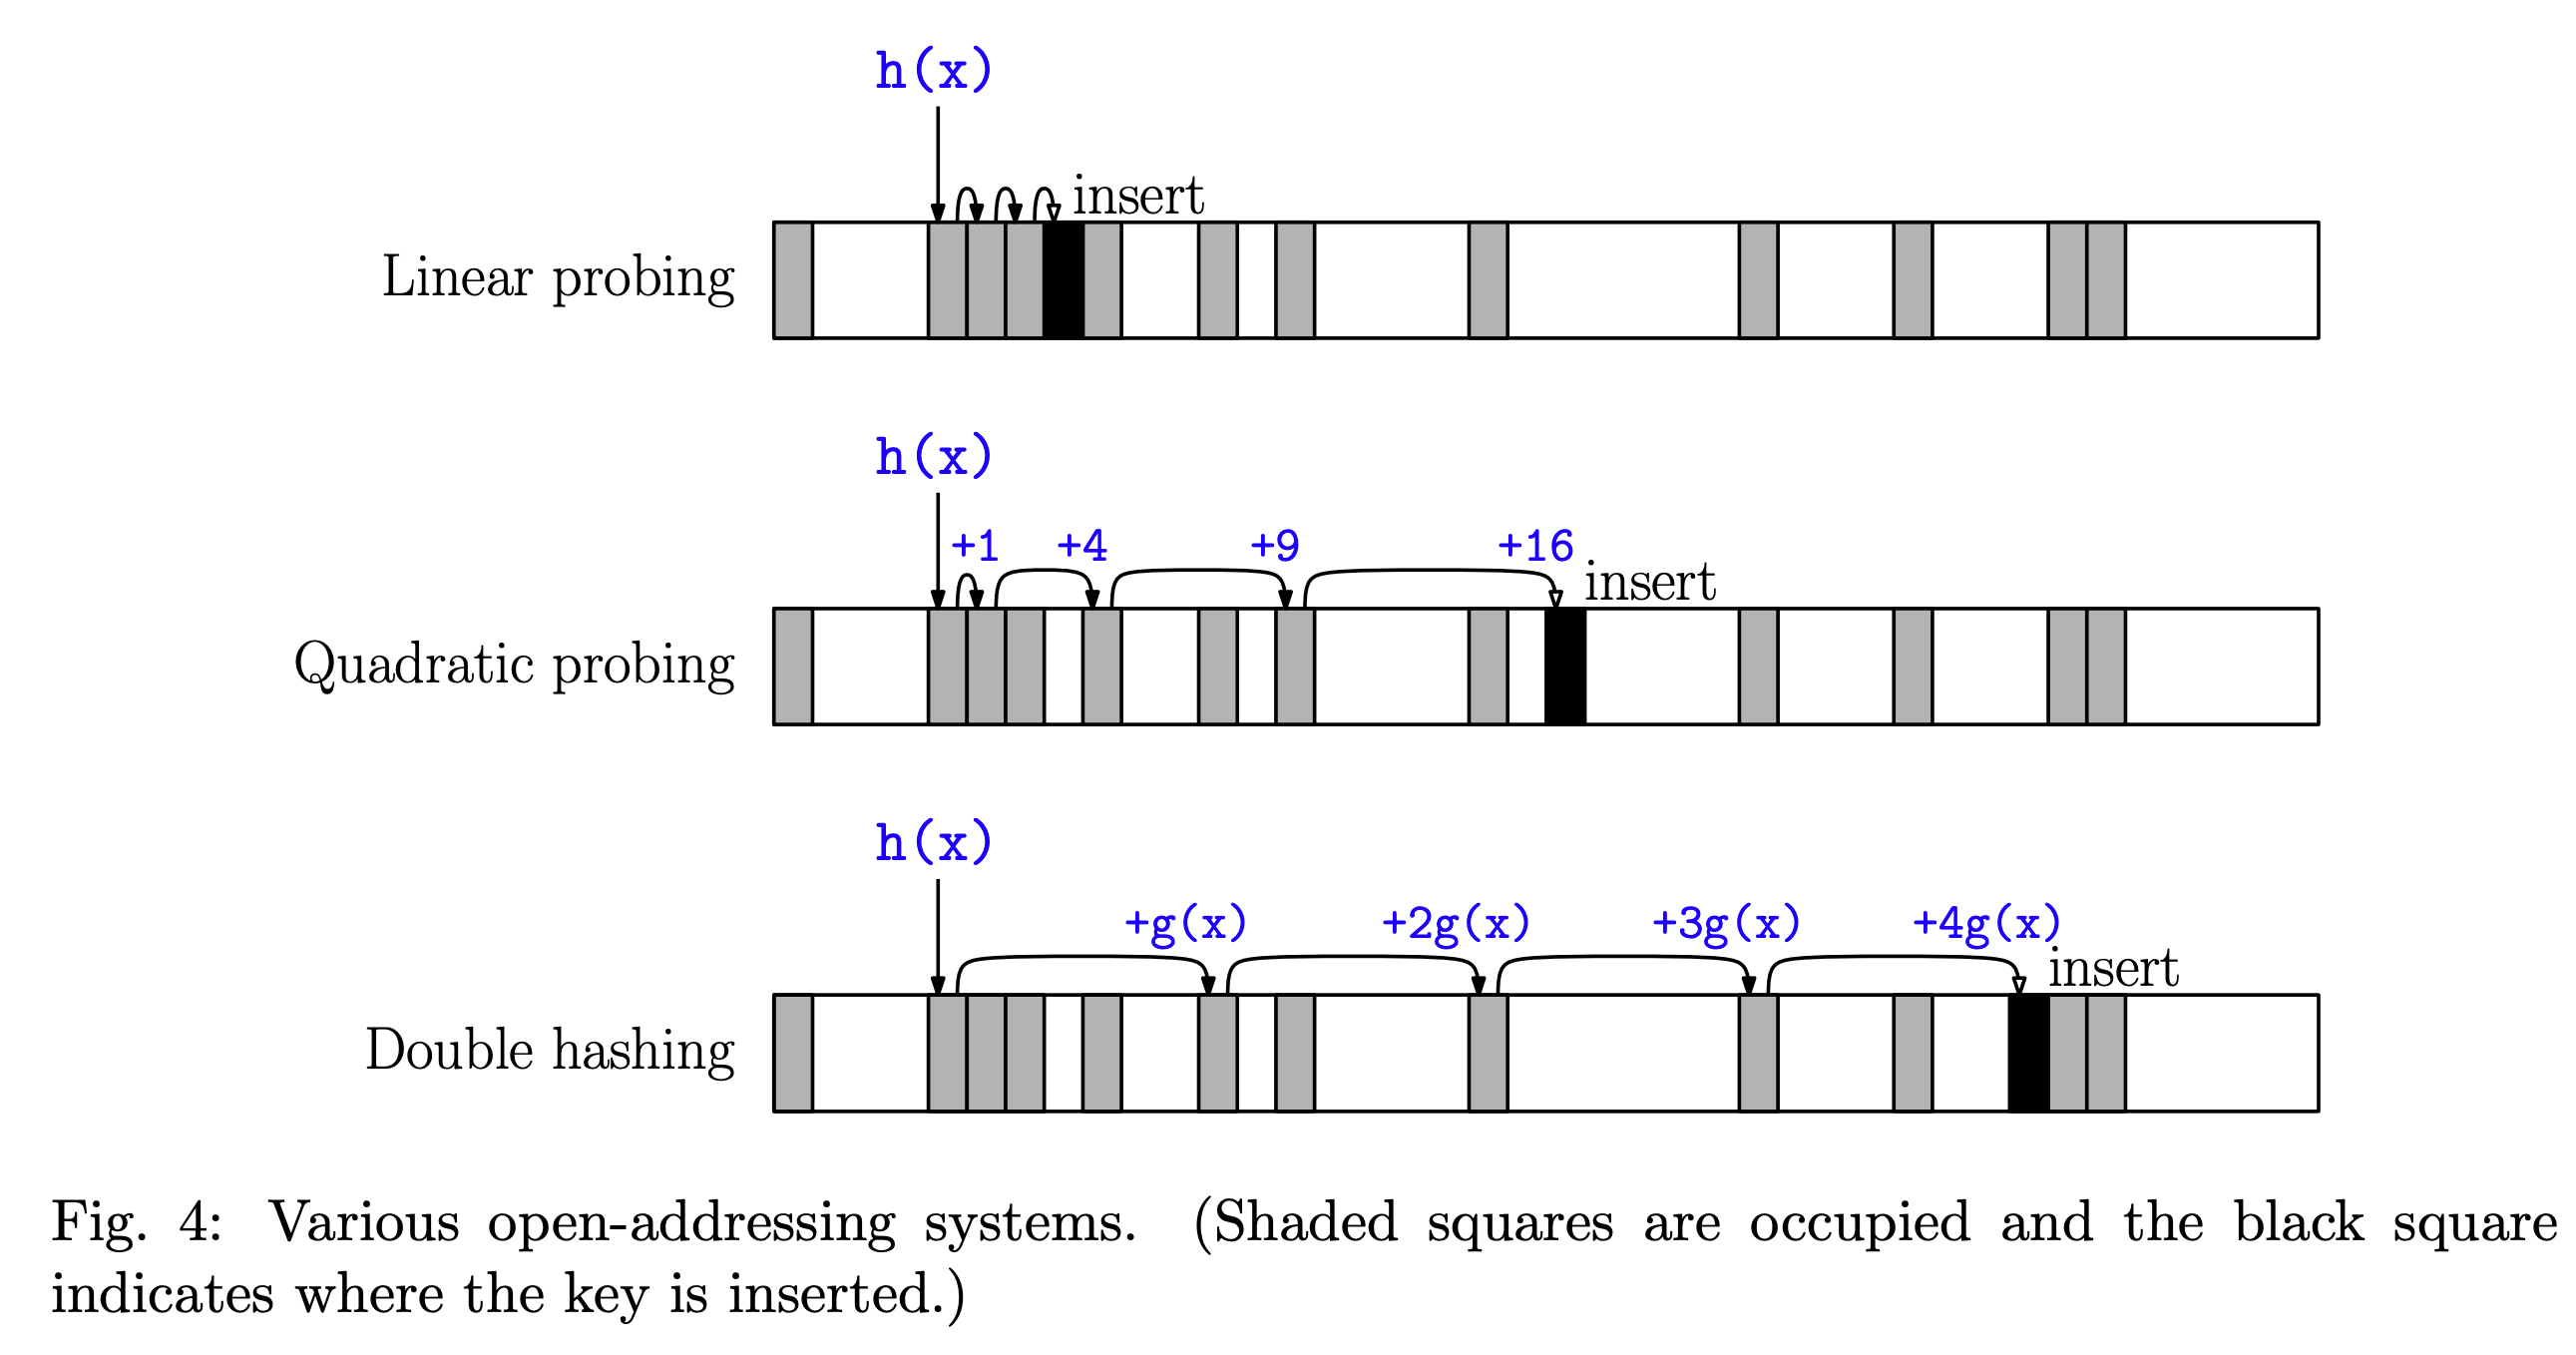
\includegraphics[width=\textwidth]{HashProbe}
  Successful search expected cost: $(\frac{1}{\lambda}\ln(\frac{1}{1 - \lambda}))$ \quad Unsuccessful serach expected cost: $(\frac{1}{1 - \lambda})$ \\ \\
  Deletition can be tricky since if we delete a node in the probe sequence, we cannot find the latter elements in that probe sequence. To resolve this, we create a special value called \textit{deleted} meaning that that slot is available for insertion but search method can continue searching the probe sequence until it finds the target element or reaches an empty cell \\
  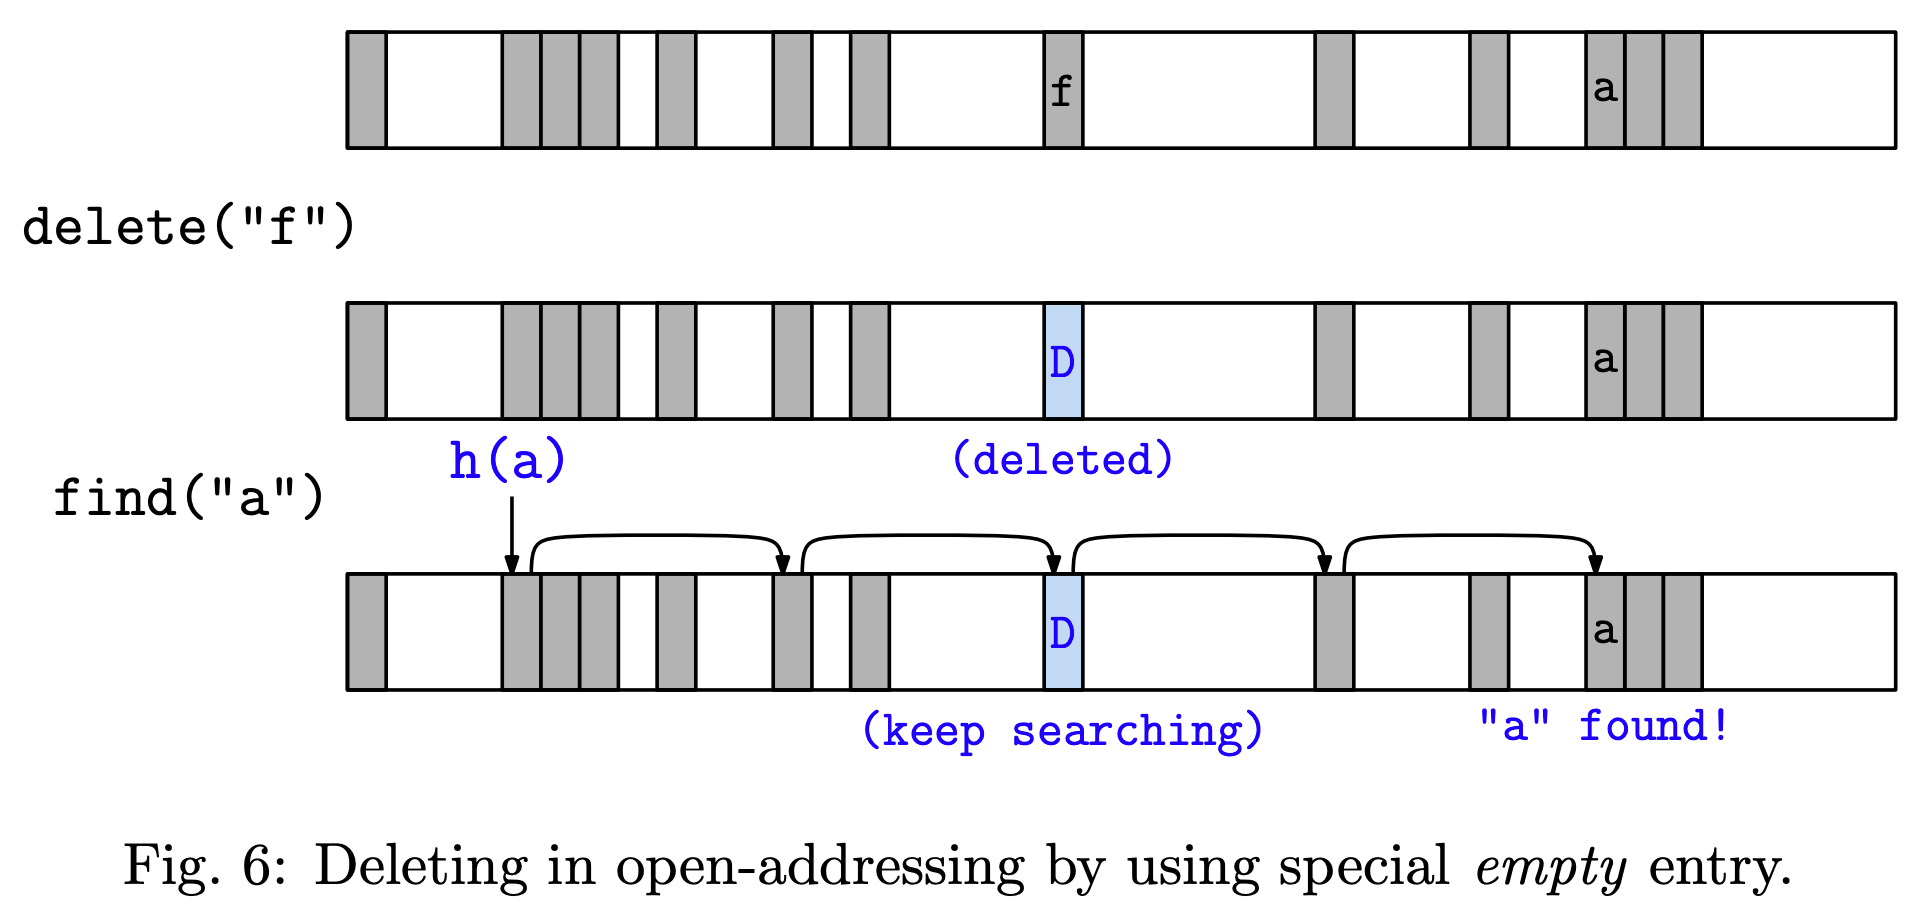
\includegraphics[width=\textwidth]{HashDeletion}
  However, this solution makes can make the search path extremely long (even if the load factor is low). Another possible solution is to bring up the latter elements of the probe sequence up after deleting an element, but that makes deletion take longer.\\
  \newpage
  \section{Extended BST and Scapegoat Trees}
  \subsection{Extended BST}
  Key are in external nodes and internal nodes have splitters with the property that all external nodes $x \leq s$ on left and $x > s$ on right\\
  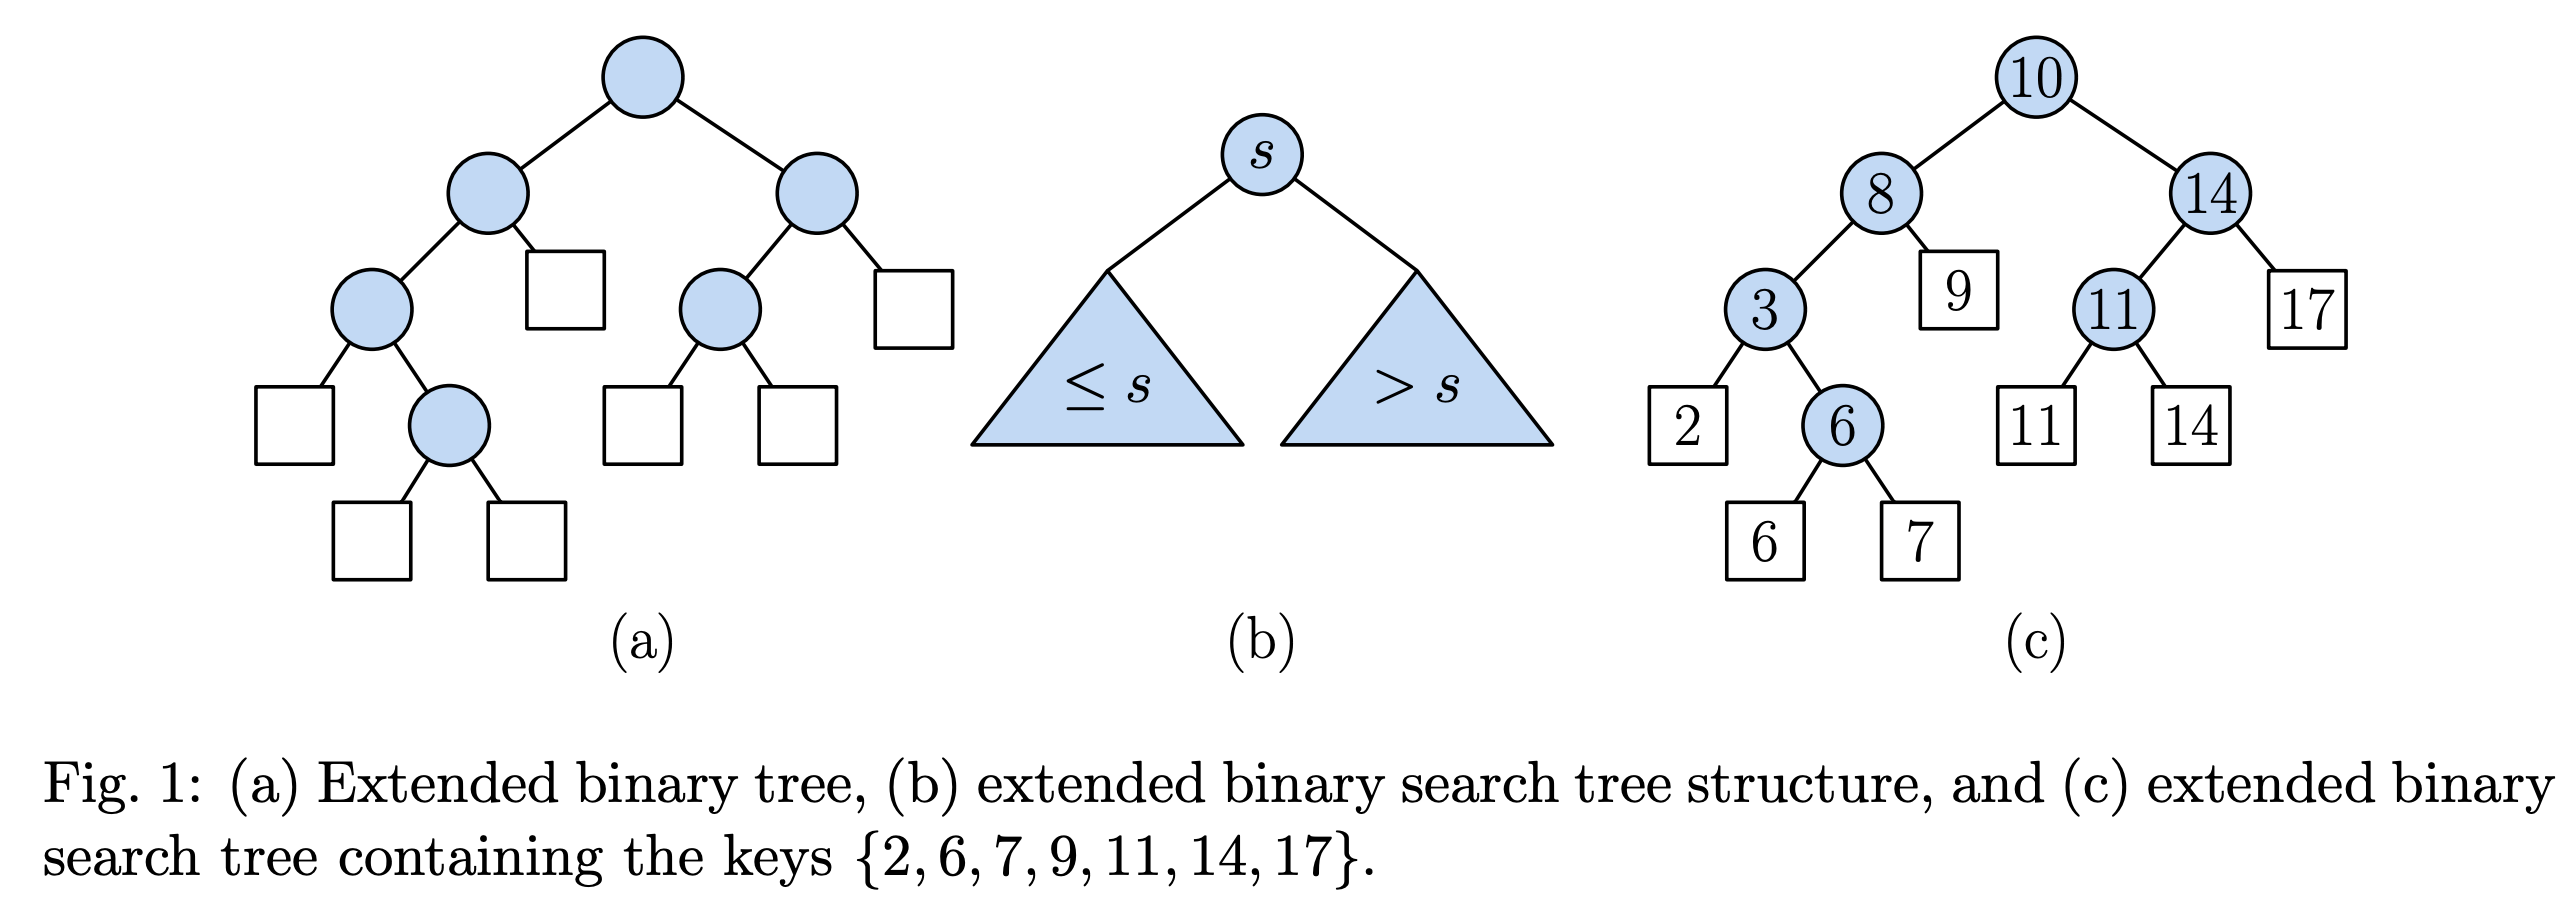
\includegraphics[width=\textwidth]{ExtendedBST}
  Find(Key x, Node P): initial call find(x, root) then 
  \begin{itemize}[noitemsep]
    \item if $x \leq p.key$ recurse on p.left
    \item else recurse of p.right
    \item once at external node u, test if $x = u.key$ \\
  \end{itemize}
  Insert(Key x, Value v, Node p): returns reference to root of updated subtree where x was inserted. Initial call insert(x, v, root) then
  \begin{itemize}
    \item if $x \leq p.key$ then recurse on p.left
    \item else recurse on p.right
    \item if empty tree craete external node with x and return it
    \item otherwise create an external node with x and an internal to split x and p.key with the value min(x, p.key)
  \end{itemize}
  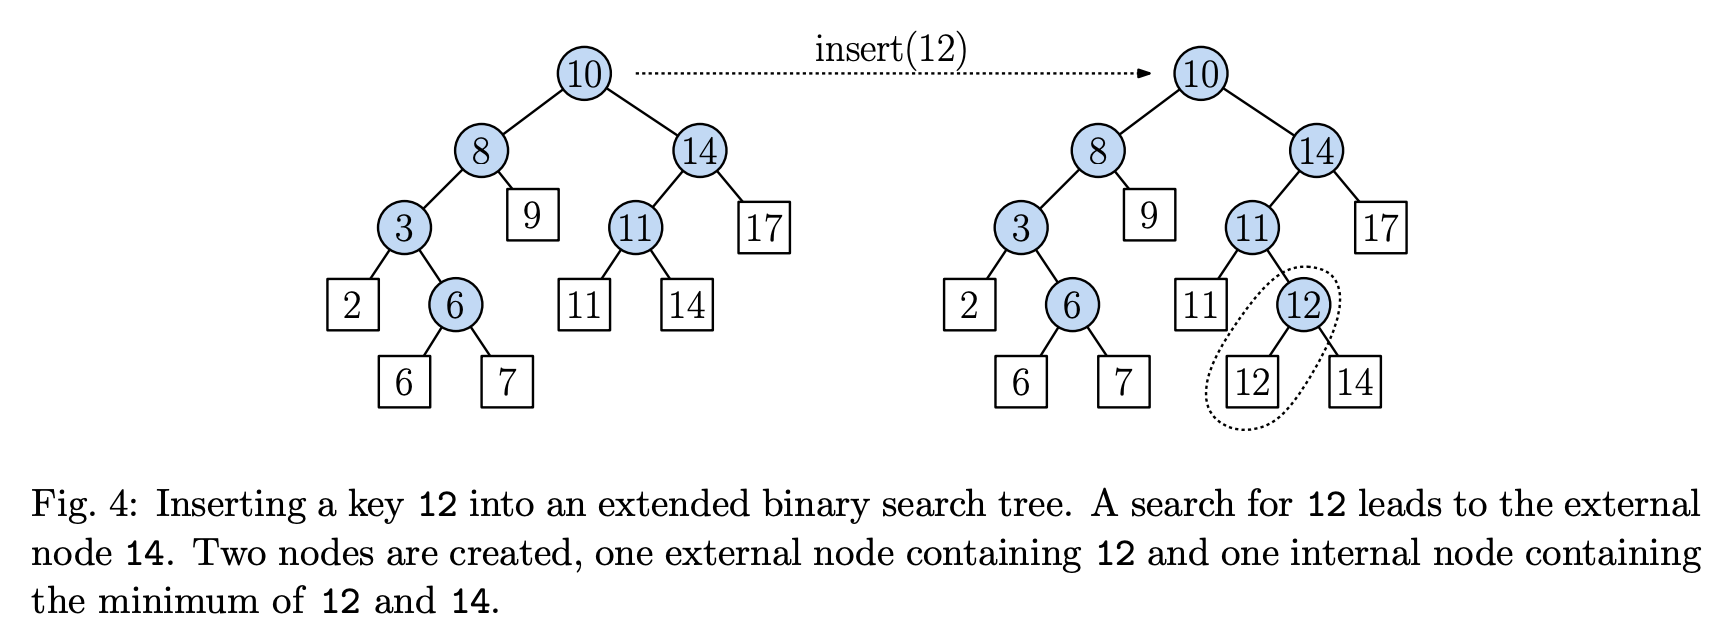
\includegraphics[width=\textwidth]{ExtendedBSTInsert}
  \newpage
  Delete(Key x, Node p): returns the root of the updated subtree from which x is deleted. Initial call delete(x, root) then
  \begin{itemize}
    \item traverse through left or right subtree accordingly
    \item if x is root, delete the external node
    \item otherwise delete the external node and its parent and return a reference to the other child of parent \\
  \end{itemize}
  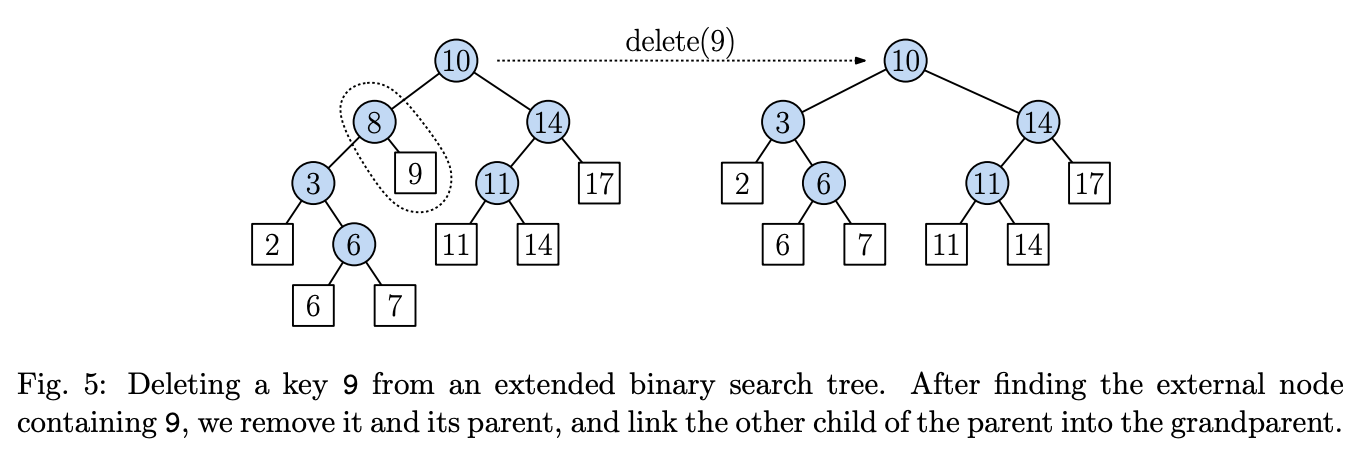
\includegraphics[width=\textwidth]{ExtendedBSTDeletion}
  Expected height is O(logn) so dictionary operations are expected to take O(logn)
  \subsection{Scapegoat Tree}
  Do not rely on rotations. Instead rebuild subtrees with poor balance. Nodes only contain key, value, left, and right and height will always be O(logn)\\
  Scapegoat Tree nodes have to store 2 values: n (number of keys in the tree) and m (upper bound size of tree)
  \begin{itemize}[noitemsep]
    \item Whenever we insert a key, we increment both n and m
    \item Whenever we delete a key, we only decrement n and do not change m
    \item This means that $m \leq n$
    \item Whenever $m > 2n$ that means number of deletes exceeds number of nodes in subtree so we rebuild it \\
  \end{itemize}
  Rebuild: Perform inorder traversal over all nodes in the scapegoat subtree rooted at p with k nodes and stored result in an array. Then recursively extract mins from the array. This will take O(k)
  \begin{lstlisting}
    BinaryNode buildSubtree(Key[] A, int i, int k) {
      if (k == 0) return null
      else {
        int m = ceiling(k/2);
        BinaryNode p = new BinaryNode(A[i+m]);
        p.left = buildSubtree(A, i, m);
        p.right = buildSubtree(A, i+m+1, k-m-1);
        return p;
      }
    }
  \end{lstlisting}
  Find(Key x): Exactly the same as BST find. Height of tree will never exceed $\log_{3/2}n$ so run time is guaranteed to be O(logn)\\ \\
  Deletion(Key x): Standard BST delete but when $m > 2n$ rebuild entire tree and set $m = n$\\ \\
  \newpage
  Insertion: Standard BST insert but need to 
  \begin{itemize}[noitemsep]
    \item monitor the depth of the inserted node. If depth $> \log_{3/2}m$ that means one of the nodes in its search path is unbalanced
    \item Traverse up through search path and if at any point $\frac{size(u.child)}{size(u)} > \frac{2}{3}$ then we rebuild u
    \item Intuition is that this subtree has twice as many nodes as siblings so we should trigger a rebuild\\
  \end{itemize}
  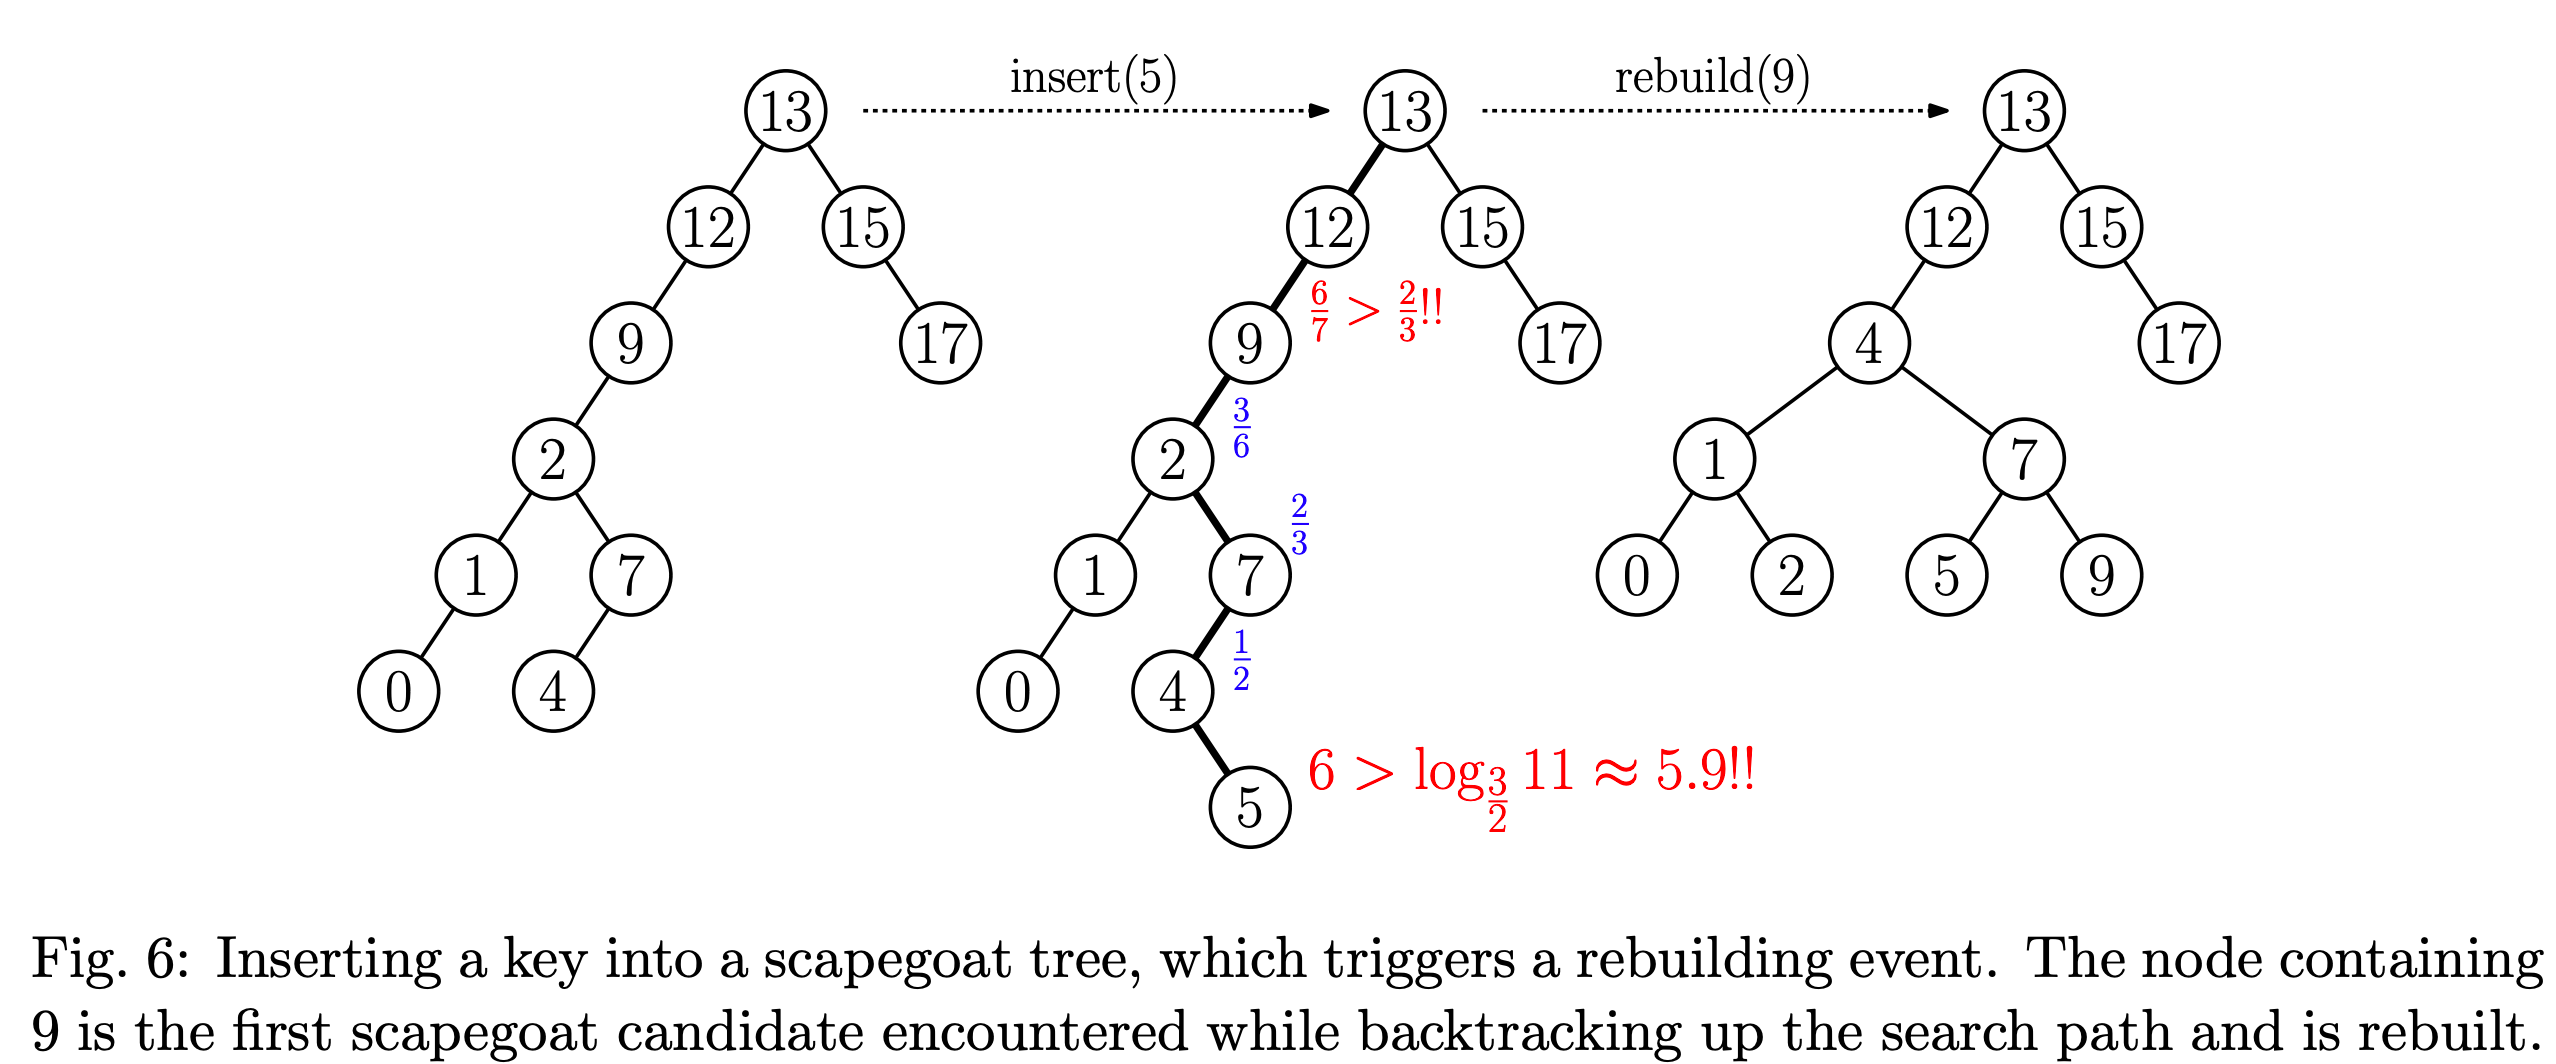
\includegraphics[width=\textwidth]{ScapegoatInsertion}
  Proof that if the depth of a node p is $> log_{3/2}n$ then p has an ancestor (possibly p itself) that is a scapegoat candidate
  \begin{itemize}[noitemsep]
    \item Proof by contradiction: assume that all nodes in the path have $size(u.child) \leq \frac{2}{3} size(u)$
    \item since the root has n nodes, we have $size(p) \geq (\frac{2}{3}^{k})n$ for the inserted node p
    \item since size(p) $\geq 1$ we have $1 \geq (\frac{2}{3}^{k})n \rightarrow k \leq log_{3/2}n$ which is a contradiction since p's depth $ > log_{3/2}n$ \\ 
  \end{itemize}
  Calculating size(u): we need to find the size of both of u's children (u' and u'') so now size(u) = 1 + u' + u''. However, cost of counting process can be accounted for in the rebuilding process (we have to count these nodes anyways)\\
  Alternate idea of counting: store size value in nodes so that
  \begin{center}
    size(u) = (u == null ? 0 : size(u.left) + size(u.right));
  \end{center}
  Height can also be updated with this idea with
\begin{center}
  height(u) = (u == null ? 0 : 1 + max(height(u.left), height(u.right)))
  \end{center}
  \newpage
  \section{Geometric Data Structures}
  Goal is to store large datasets of geometric objects(points, lines, shapes) in order to answer queries on them. These queries don't focus on exact matches and instead focus on "close to", "contained with", or "overlapping with"\\ \\
  Nearest Neighbor Search: store set of points so giveen a query point q it is possible to find the closest point of the set to q\\
  Range Searching: store set of points so that given a query region R (e.g. circle) it is possible to count all points of set that are in R\\
  Point Location: store subdivision of space into disjoint regions so that given a query point q, it is possible to determine which region has q efficiently\\
  Intersection Searching: store collection of geometric objects so that given a query of objects R of the same type, report all objects in set that intersect with R\\
  Ray shooting: store collection of objects so that given an query ray, ran determine whether ray hits any object in set, and which it hits first\\
  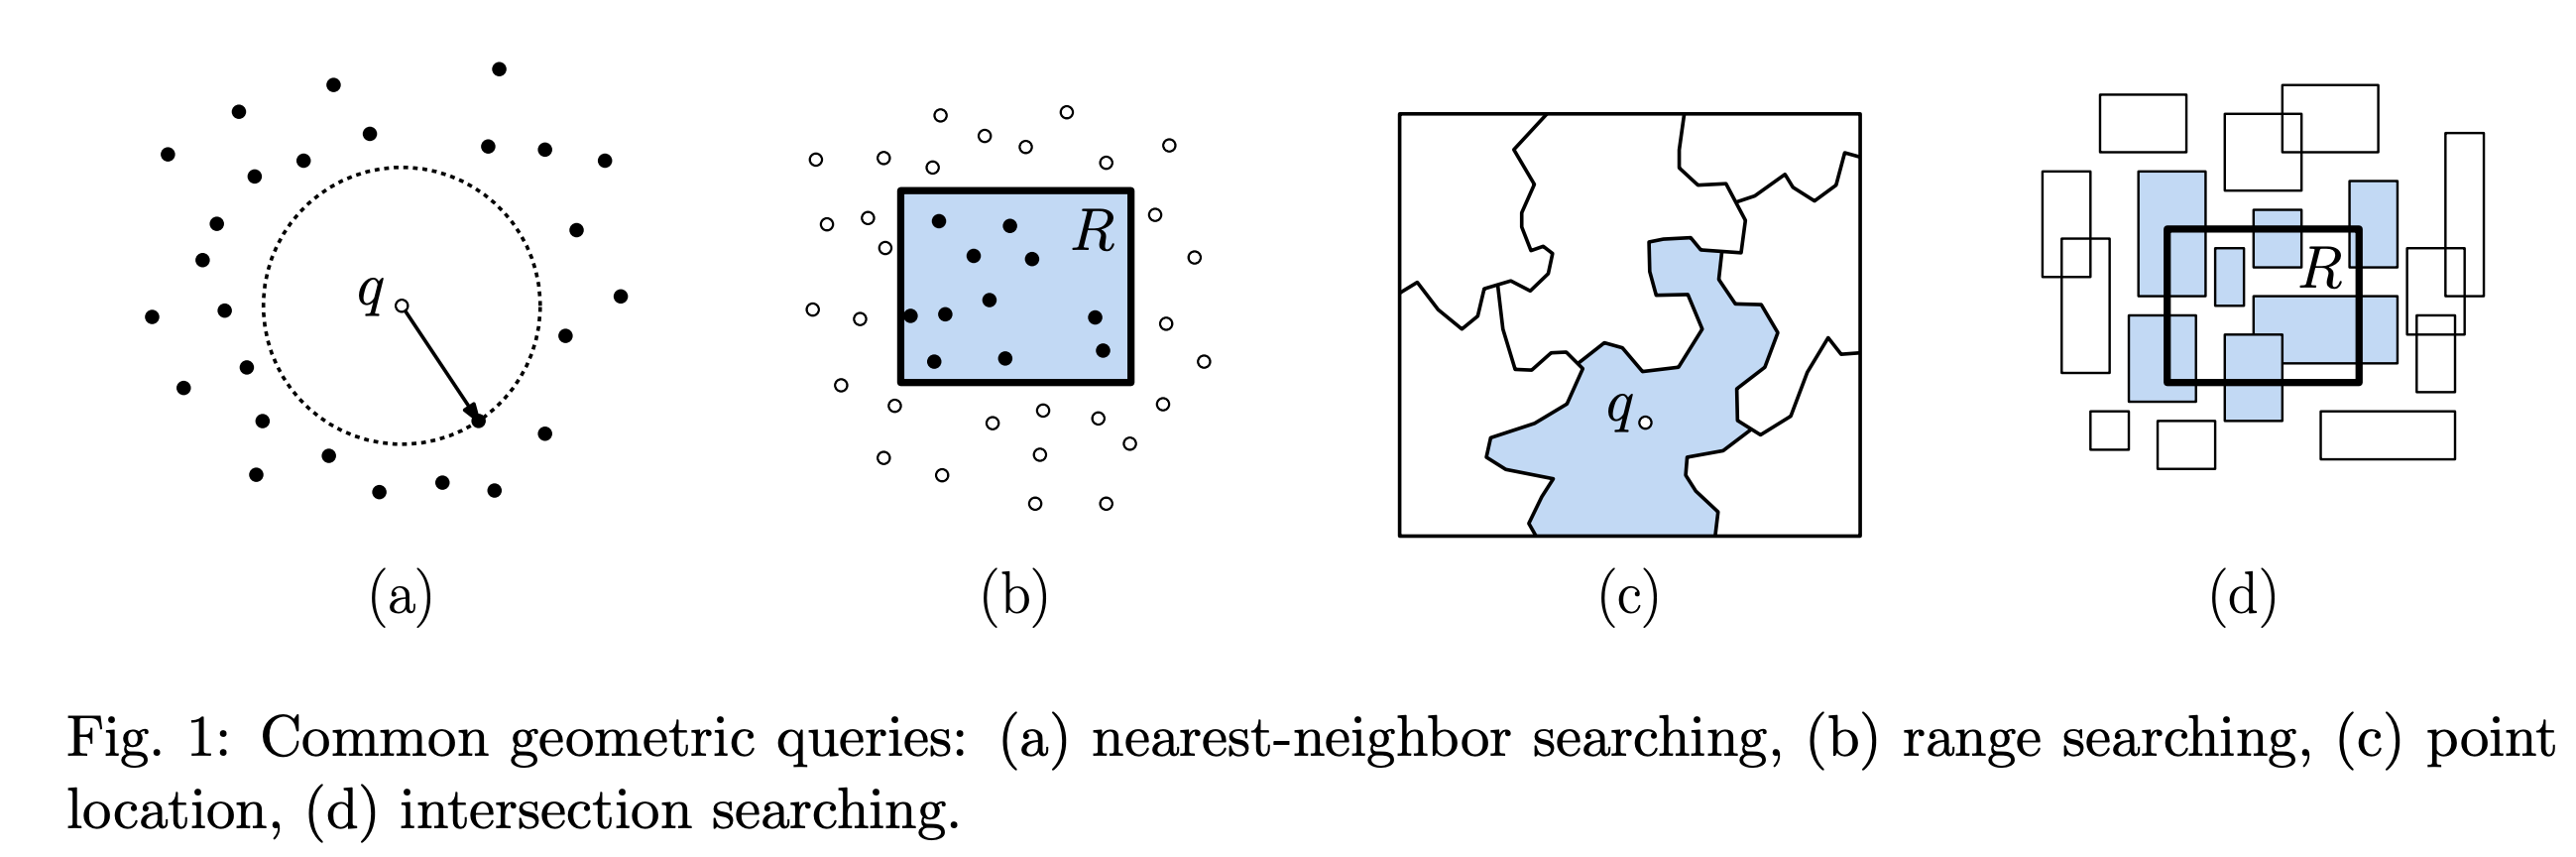
\includegraphics[width=\textwidth]{GeometricQueries}
  Point Representation: Can represent as 2d array with n points of d dimension
  \begin{center}
    float[][] p = new float[n][d]
  \end{center}
  Can also represent using a Point class
  \begin{lstlisting}
    public class Point {
      private float[] coord;    // coordinate storage
      public Point(int dim) { ... } // constructor

      public int getDim {return coord.length} //dimension of point
      public float get(int i) {return coord[i]}

      public boolean equals(Point p) { ... }
      public float distanceTo(Point p) { ... }
    }
  \end{lstlisting}
  \newpage
  \noindent Point quadtree: Generalizing for a 2d coordinate plane, each node has 4 children (NW, NE, SW, SE). Traverse through tree based on coordinate x and y comparison. This creates rectangle regions called cells that can be recursively split. Can be extended to generalize points with d dimensions using $2^{d}$ child nodes but that takes up a lot of space\\
  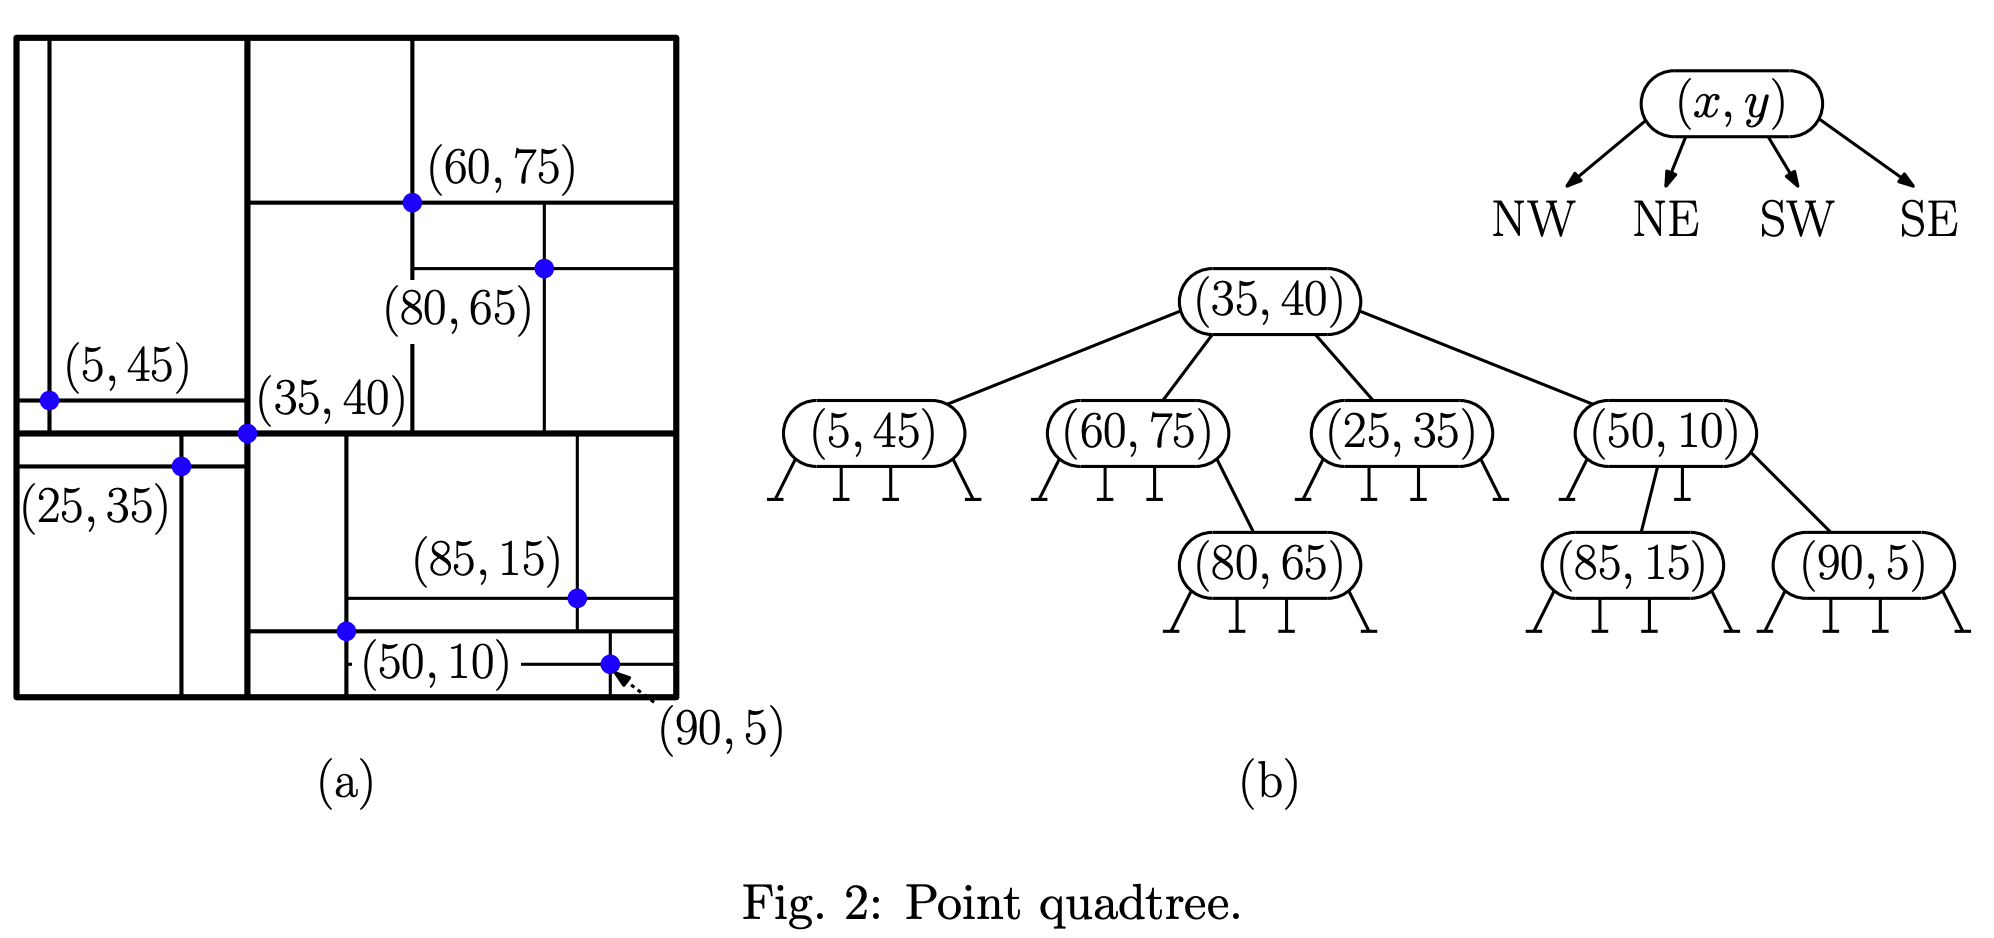
\includegraphics[width=\textwidth]{PointQuadtree}
  Point kd-trees: represent multi-dimensional points with using a binary tree. Whenever a new point is inserted into a node, we split the cell by a splitting line (0 to d-1). Cutting dimension is chosen by alternating among possible axes at each new level of the tree. 
  \begin{lstlisting}
    class KDNode {
      Point point;    // splitting point
      int cutDim;     // cutting dimension
      KDNode left;
      KDNode right;

      KDNode(Point point, int cutDim) {
        this.point = point;
        this.cutDim = cutDim;
        left = right = null;
      }

      boolean inLeftSubTree(Point x) {  // is in left subtree
        return x[cutDim] < point[cutDim]
      }
    }
  \end{lstlisting}
  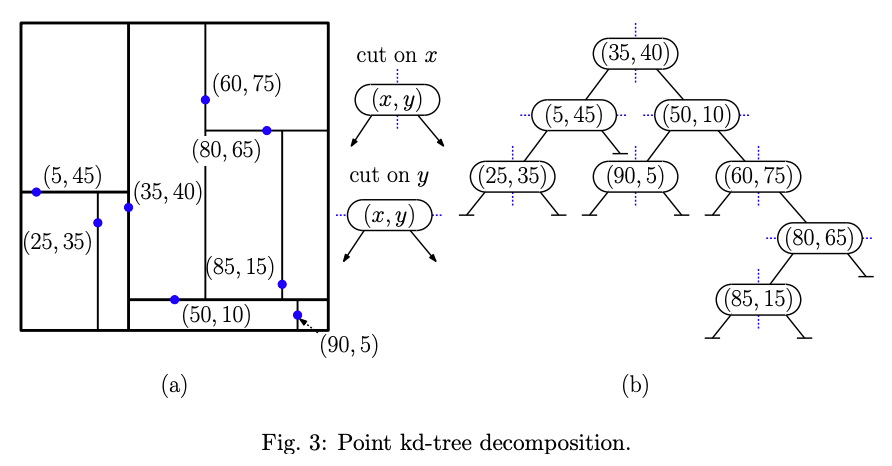
\includegraphics[width=\textwidth]{PointKDTree}
  Insertion into kd-tree: Same as BST. When we create a node containing the point, we assign its cutting dimension. Initial call root = insert(x, root, 0).
  \begin{lstlisting}
    KDNode insert(Point x, KDNode p, int cutDim) {
      if (p == null) p = new KDNode(x, cutDim);
      else if (p.point.equals(x)) throw Exception("duplicate point");
      else if (p.inLeftSubtree(x)) p.left = insert(x, p.left, (p.getDim + 1) \% x.getDim());
      else p.right = insert(x, p.right, (p.cutDim + 1) \% x.getDim());
      return p;
    }
  \end{lstlisting}
  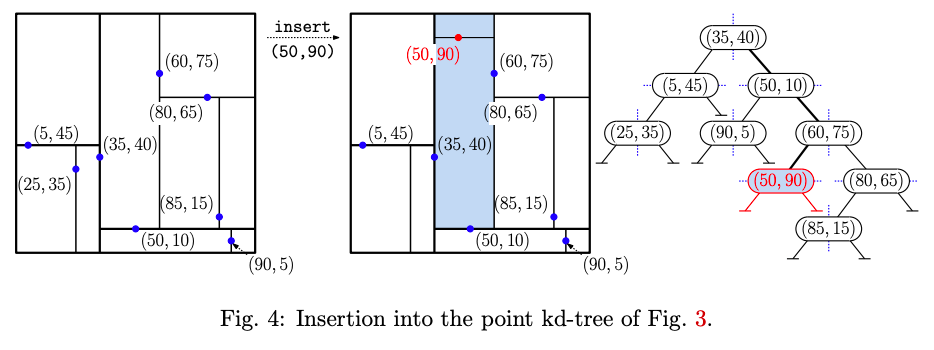
\includegraphics[width=\textwidth]{KDInsertion}
  \newpage
  Deletion in kd-tree: Issue with finding a replacement point since each adjacent level of tree has different cutDim value. Need to use an auxiliary meethod findMin()\\
  findMin(p, cutDim): if the node we are testing has the same cutDim value, then we recurse on left side. Otherwise we have to use another auxiliary method minAlongDim() which returns whicever point p1 or p2 is the smallest among coordinate cuttDim.
  \begin{lstlisting}
    Point findMin(KDNode p, int i) {
      if (p == null) return null;
      if (p.cutDim == i) {
        if (p.left == null) return p.point;
        else return findMin(p.left, i);
      } else {
        Point q = minAlongDim(p.point, findMin(p.left, i), i);
        return minAlongDim(q, findMin(p.right, i), i);
      }
    }

    Point minAlongDim(Point p1, Point p2, int i) {
      if (p2 == null || p1[i] <= p2[i]) return p1;
      else return p2;
    }
  \end{lstlisting}
  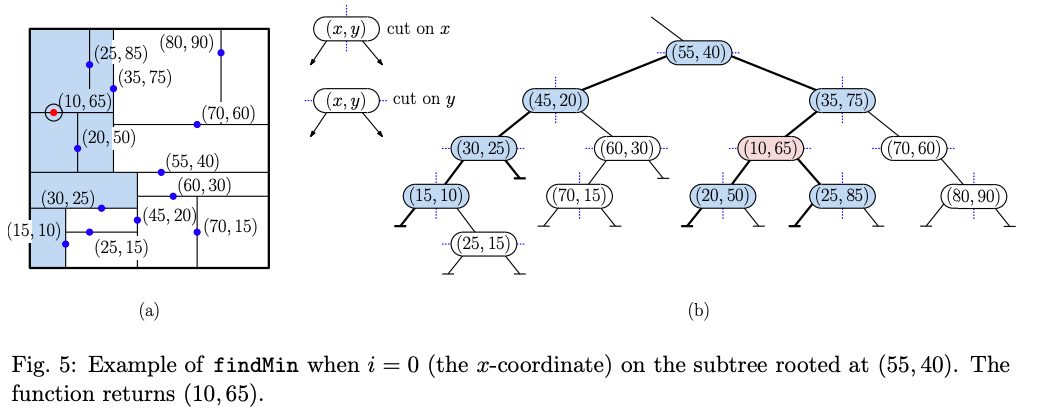
\includegraphics[width=\textwidth]{KDTreeFindMin}
  \newpage
  Another issue of deletion for kd-tree is that if the deleted node has a single child, we can't just bring that child subtree up since it has a different cutDim parity. Solution is to use findMin() to get the smallest x-coordinate or smallest y-coordinate in the right subtree. If the right subtree is empty then we find the min on the left subtree and and move the left subtree to the right subtree, setting the left-child pointer to null. Issue with finding the max on the left subtree is that if another point has the same coordinate value, it messes up the invariant (left subtree has points $<$ and right subtree has points $\geq$)
  \begin{lstlisting}
    KDNode delete(Point x, KDNode p) {
      if (p == null) throw Eception("point DNE");
      else if (p.point.equals(x)) {
        if (p.right != null) {
          p.point = findMin(p.right, p.cutDim);
          p.right = delete(p.point, p.right)
        } else if (p.left != null) {
          p.point = findMin(p.left, p.cutDim);
          p.right = delete(p.point, p.left);
          p.left = null;
        } else if (p.inLeftSubTree(x)) p.left = delete(x, p.left);
        else p.right = delete(x, p.right);
        return p;
      }
    }
  \end{lstlisting}
  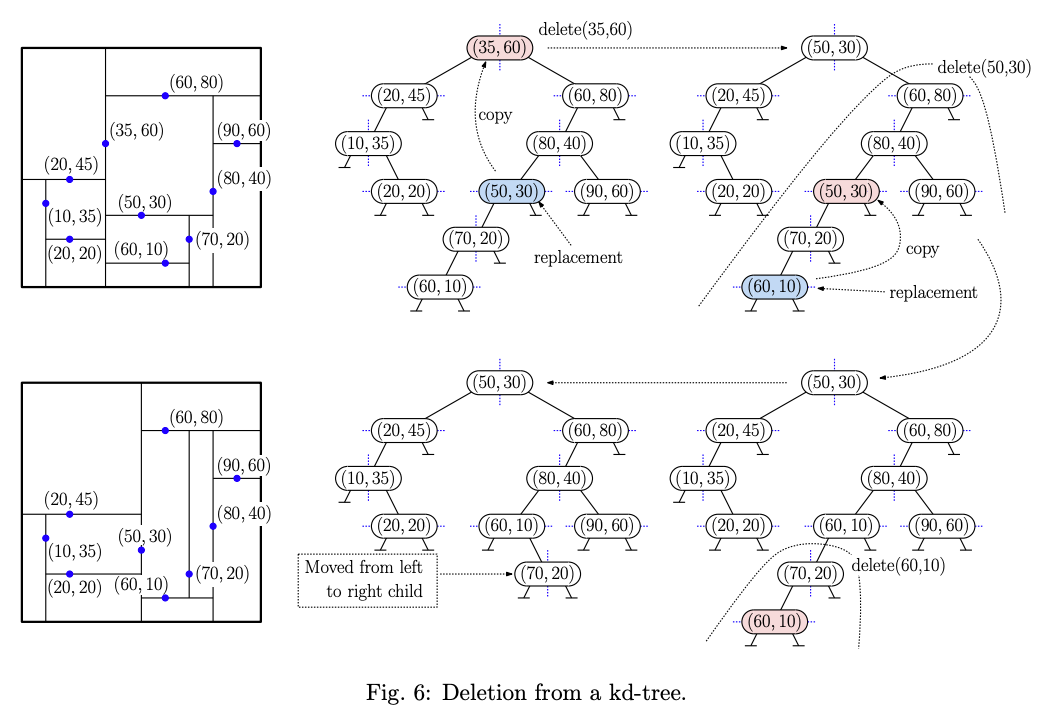
\includegraphics[width=\textwidth]{KDTreeDeletion}
  \newpage
  \noindent Analysis: Storage O(n). We treat the number of dimensions d as a constant so O(dn) = O(n)\\
  Height is O(logn). Since we chose replacement nodes in a biased way height can mutate to be $O(\sqrt{n})$
  We can build a kd-tree by choosing the splitting point to be the median according to x-coordinates. Then we split each partition using their medians according to y-coordinates. Keep recursing until done and height will be O(logn). Building takes O(nlogn)\\ \\
  Range Queries: find how many points lie in a given region R. Use a kd-tree to store points. We will need a class for storing multi-dimensional rectangles which consists 2 points (low and high). A point q lies within the rectangle if $low[i] \leq q[i] \leq high[i]$.\\
  Notable methods:\\ 
  boolean contains(Point q): returns true iff point q is contained within this rectangle\\
  boolean contains(Rectangle c): returns true iff this rectangle contains rectangle c. Have to test containment on all intervals defining each of the rectangles' sides:
  \begin{center}
    $[c.low[i],c.high[i]] \in [low[i], high[i]]$, for all $0 \leq i \leq d - 1$
  \end{center}
  boolean isDisjointFrom(Rectangle c): returns true iff rectangle c is disjoint from this rectangle. Have to test whether any of the defining intervals are disjoint
  \begin{center}
    $r.high[i] < c.low[i] or r.low[i] > c.high[i]$, for any $0 \leq i \leq d-1$
  \end{center}
  float distanceTo(Point q): returns minimum Euclidean distance from q to any point on rectangle. Computed by computing distance from coordinate q[i] to rectangle's ith defining interval
  \begin{center}
    $\sqrt{\sum_{i=0}^{d-1}(distance(q[i], [low[i], high[i]]))^{2}}$
  \end{center}
  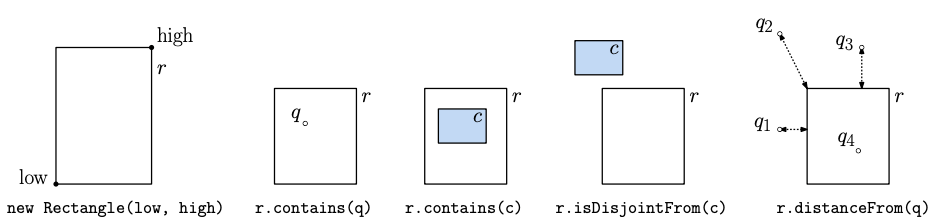
\includegraphics[width=\textwidth]{RangeQueriesMethods}
  \newpage
  Rectangle leftPart(int cd, Point s): Given a rectangle r and a splitting point s, we want to cut the rectangle into two sub-rectangles by a line that passes through the splitting point. leftPart returns a rectangle whose low point is the same as r.low and whose high point is the same as r.high, except that the cd-th coordinate is set to s[cd].
  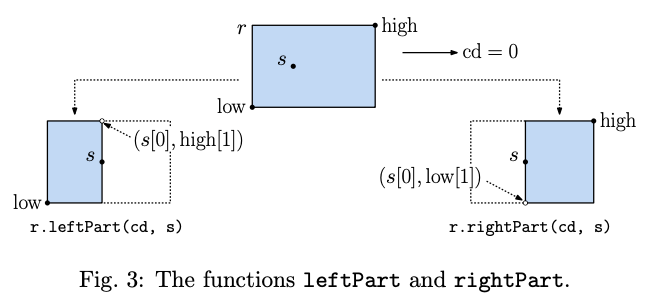
\includegraphics[width=\textwidth]{RangeQueriesLeftPart}
  Answering Range Query: assume that each node p has a member p.size indicating the number of points lying within the tree. This can be easily updated as points are inserted and deleted. \\
  The rangeCount(r, p, cell) function operates recursively, returning a count of the number of points that lie in range r. Initial call is rangeCount(r, root, boundingBox) where boundingBox bounds the entire kd-tree. If the 
  \begin{itemize}[noitemsep]
    \item if we fall out of tree there is nothing to count
    \item if the current node's cell is disjoint from the query range, return 0
    \item if query range completely contains cell, return p.size
    \item if the range partially overlaps the cell, apply function recursively to each of our two children
  \end{itemize}
  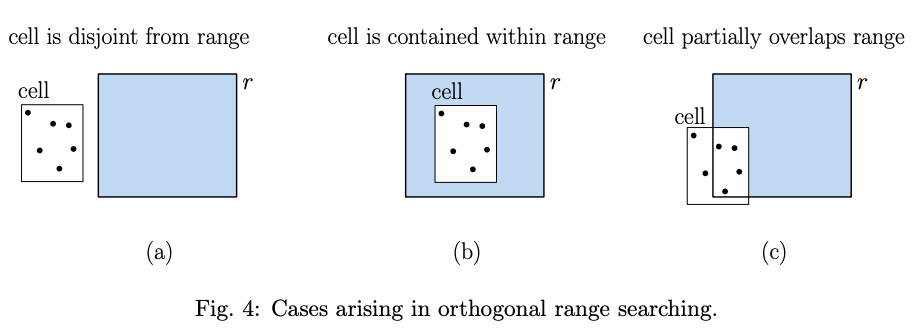
\includegraphics[width=\textwidth]{RangeCount}
  \newpage
  \begin{lstlisting}
    int rangeCount(Rectangle r, KDNode p, Rectangle cell) {
      if (p == null) return 0;
      else if (r.isDisjointFrom(cell)) return 0;
      else if (r.contains(cell)) return p.size;
      else {
        int count = 0;
        if (r.contains(p.point)) count++;
        count += rangeCount(r, p.left, cell.leftPart(p.cutDim, p.point));
        count += rangeCount(r, p.right, cell.rightPart(p.cutDim, p.point));
        return count;
      }
    }
  \end{lstlisting}
  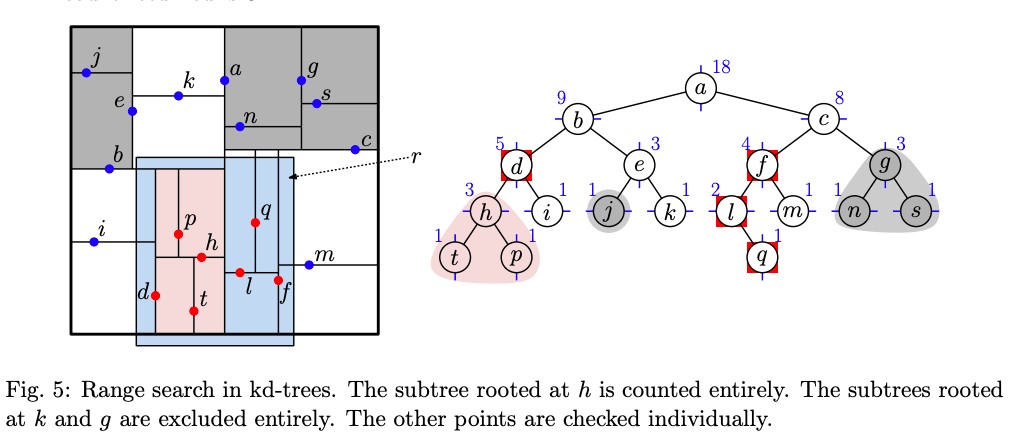
\includegraphics[width=\textwidth]{RangeSearchExample}
  Range Queries can be answered in $O(\sqrt{n})$ time \\
  A node is processed (both children visited) iff the call overlaps the range without being contained within the range (stabbed by the query). To bound total number of nodes processed in search, we count the total number of nodes whose cells are stabbed by the query rectangle. \\
  Given any balanced kd-tree with n points, any vertical or horizontal line stabs $O(\sqrt{n})$ cells of the tree. \\
  Since the tree is balanced, its height is O(logn) $\approx$ lgn\\
  Consider only stabbing using vertical or horizontal lines instead of rectangles. When processing a node, the line will stab one of the two children. This means when alternating between x and y, at most two of the possible four grandchildren of each node is stabbed.\\
  Since we have an exponentially increasing number, total sum is dominated by the last term
  \begin{center}
    $2^{h/2} \approx 2^{(lgn)/2} = \sqrt{n}$
  \end{center}
  For the rectangle case, there are 4 sides to the rectangle so $O(4\sqrt{n})$\\
  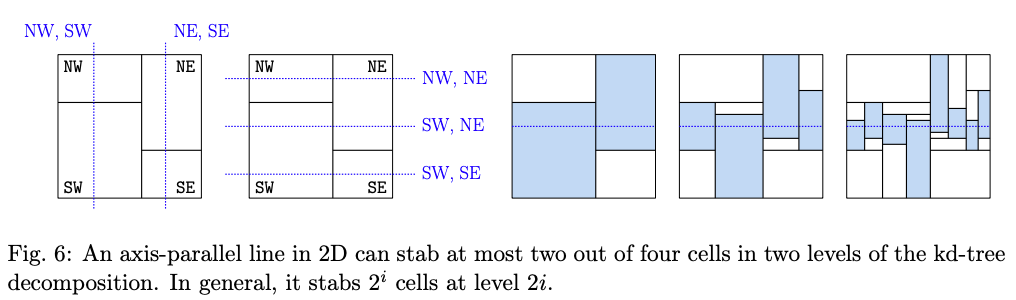
\includegraphics[width=\textwidth]{RangeQueryProof}
  Nearest-Neighbor Queries: given a set of points P storedi n a kd-tree and a query point q, return the point of P closest to q. Assume that distances are measured using Euclidea distances.
  \begin{center}
    $dist(p,q) = \sqrt{(p_{1}-q_{1})^{2} + ... + (p_{d}-q_{d})^{2}}$
  \end{center}
  May need to visit every leaf that overlaps with the range. However, number of nodes overlapping the range is usually much smaller than the total number of nodes in the tree. \\
  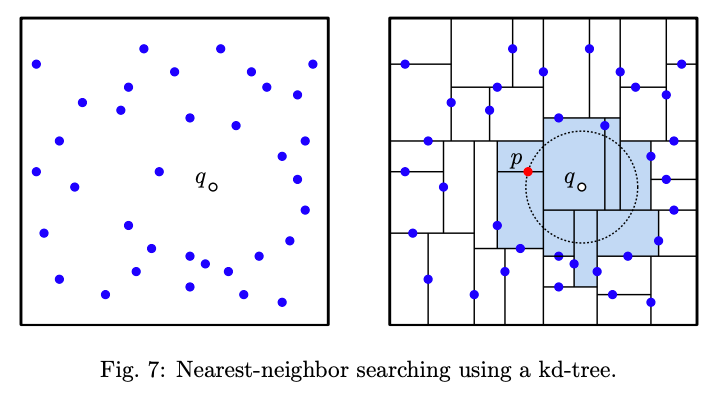
\includegraphics[width=\textwidth]{NearestNeighborExample}
  Another approach would be to find the leaf node of the kd-tree that contains q and then search this and its neighboring cells in the kd-tree. However, there might be an issue that the nearest neighbor may actually be very far away. 
  Three things to consider for range and nearest neighbor processing:
  \begin{itemize}[noitemsep]
    \item Partial results: store the intermediate results of query and update results as query proceeds
    \item Traversal order: visit the subtree first that is more likely to be relevant
    \item Pruning: Don't visit any subtree that is irrelevant
  \end{itemize}
  How Nearest-neighbor Code works:
  \begin{itemize}[noitemsep]
    \item If p is null so just return bestDist
    \item Compute the distance from p.point to q, and update bestDist as necessary
    \item either recurse of leftPart or rightPart accordingly
  \end{itemize}
  \newpage
  \begin{lstlisting}
    float nearNeighbor(Point q, KDNode p, Rectangle cell, float bestDist) {
      if (p != null) {
        float thisDist = q.distanceTo(p.point);
        bestDist = Math.min(this.Dist, bestDist);

        int cd = p.cutDim;
        Rectangle leftCell = cell.leftPart(cd, p.point);
        Rectangle rightCell = cell.rightPart(cd, p.point);

        if (q[cd] < p.point[cd]) {
          bestDist = nearNeighbor(q, p.left, leftCell, bestDist);
          if (rightCell.distanceTo(q) < bestDist) bestDist = nearNeighbor(q, p.right, rightCell, bestDist);
        } else {
          bestDist = nearNeighbor(q, p.right, rightCell, bestDist);
          if (leftCell.distanceTo(q) < bestDist) bestDist = nearNeighbor(q, p.left, leftCell, bestDist);
        }
      }
      return bestDist;
    }
  \end{lstlisting}
  Worst case is we need to visit every node but this is typically not the case. Usually $O(2^{d} + logn)$ where d is the dimension of the space. Intuition is that we need to visit some set of nodes in the neighborhood and require logn to descend tree
  \newpage
  \section{Memory Management}
  2 principles to dynamic memory allocation. 
  \begin{itemize}[noitemsep]
  \item Stack where arguments and local variables are pushed onto when a procedure is called. These are popped when a procedure returns. 
  \item Heap where objects are allocated and deallocated, fragmenting the heap into pieces.
  \end{itemize}
  Issues with memory allocation:
  \begin{itemize}[noitemsep]
    \item Explicit deallocation (languages like C) are a burden for programmers. Blocks of memory may be leaked (inaccessible and has not be deallocated). Another issue of aliasing where two pointers refer to the same block of memory leading to the issue of when one pointer is released, the other still references that chunk of memory
    \item Implicit deallocation (Languages like Java) the system determines which objects are no longer accessible using garbage collection but put a burden on the memory allocation system
  \end{itemize}
  Explicit Allocation/Deallocation: one case where explicit deallocation is easy to handle: when all objects being allocated are of the same size (array). Very easy to allocate a contiguous space in heap and blocks are linked together. However for objects of varying sizes, we can run into an issue of external fragmentation, essentially wasting space\\ 
  Explicit allocation works in that when allocating a block, we search through the list of available blocks of memory that is large enough. There are two strategies to this:
  \begin{itemize}
    \item First-fit: search available blocks sequentially until find a large enough space
    \item Best-fit: search all available blocks and insert into smallest block large enough
  \end{itemize}
  Best-fit usually performs worse than first-fit (first-fit is faster to execute and best-fit tends to produce a large amount of fragmentation by selecting blocks taht are barely larger than the request size, leaving tiny residual blocks). One possible solution to reduce fragmentation is just make the requested block take up all the available space, keeping the list of available blocks free of tiny fragments and speeding up search time. However this creates internal fragmentation.\\
  When deallocating a block, we should merge available space to create large blocks of free space (this is called merging) but there's an issue of figuring out how to efficiently merge.\\ \\
  For each allocated blocks we record its size, inUse, and prevInUse \\
  For each available block we store these blocks in a doubly-linked circular list (avail) and has size, inUse, prevInUse, prev , next, and size2. \\ \\
  Allocation: to allocate a block, search through linked list of available blocks until find one of sufficient size. If the size pretty much fits, remove the block from the list of available blocks, updating linkage and prevInUse as necessary. If desired allocation is much smaller than the block chosen, split the block into two smaller blocks and relink as necessary.\\
  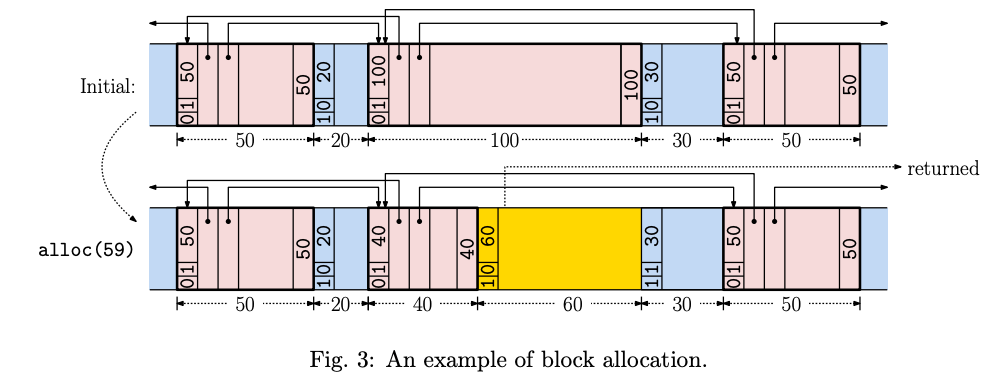
\includegraphics[width=\textwidth]{MemoryAllocation}
  \newpage
  \begin{lstlisting}
    (void *) alloc(int b) {
      b += 1;       // extra space for system overhead
      p = search available space list for block of size at least b;
      if (p == null) throw Exception("Too small");
      if (p.size - b < TOO\_SMALL) {
        avail.unlink(p);
        q = p;
      } else {
        p.size -=b;
        *(p + p.size - 1) = p.size;   // set new block's size2 field
        q = p + p.size;
        q.size = b;
        q.prevInUse = 0;
      }
      q.inUse = 1;
      (q + q.size).prevInUse = 1;
      return q + 1;   //offset link to avoid header
    }
  \end{lstlisting}
  \newpage
  Deallocation: to deallocate we check if the next block or preceding blocks are avaliable. For the next block we can find it's first word and check its inUse field. For the preceding block we just use the prevInUse field. \\
  If the prev block isn't in use, we use the size value stored in the last word to find the header values appropriately. If either of these blocks is available, merge the two blocks and update header value appropriately. If both are available, we need to delete one of these blocks from available space list. If both are in-use, we link current block to list of available blocks.\\
  There are four cases to consider for deallocation
  \begin{itemize}[noitemsep]
    \item If the following block q is available, merge with p. Update p's size and move q's record in the available space list to p using move(p,q), copying q's previous and next fields to p and appropriately update the entries in the available space list that point to q. Otherwise add p to available space list
    \item If preceding block isn't in use, merge this block with p and unlink p from the available space list
  \end{itemize}
  \begin{lstlisting}
    void dealloc(void* p) {
      p--;      // back up to the header;
      q = p + p.size;   // pointer to following block
      if (!q.inUse) {
        p.size += q.size;
        avail.move(q, p);
      } else avail.insert(p)

      p.inUsee = 0;
      *(p + p.size = 1) = p.size;

      if (!p.prevInUse) {
        q = p - *(p-1);
        q.size += p.size;
        *(q + q.size - 1) = q.size;
        avail.unlink(p);
        (q + q.size).prevInUse = 0;
      }
    }
  \end{lstlisting}
  \includegraphics[width=\textwidth]{MemoryDeallocation}
  Analysis: typically methods achieve utilization of around 2/3 storage before failing to satisfy a request so in general allocate a heap of at last 10 times size of largest block to be allocated\\ \\
  Buddy System: Long sequences of allocations and deallocations of objects of varius sizes tends to result in highly fragmented space. We can minimize this by limiting the possible sizes of blocks and their positions using well-structured allocation. Because block sizes are limited, internal fragmentation becomes an issue. \\
  Start with a block of memory whose size is a power of 2 and then hierarchically subdivide each block into blocks of equal sizes.
  \begin{itemize}[noitemsep]
    \item Sizes of all blocks are powers of 2. A request is artificially rounded up to the next power of 2
    \item Blocks of size $2^{k}$ start at memory addresses that are multiples of $2^{k}$
  \end{itemize}
  \includegraphics[width=\textwidth]{BuddySystem}
  For every block, there is exactly 1 other block with which this block can be merged (called the buddy)
  \begin{center}
    \[
      buddy_{k}(x) = \left\{
        \begin{array}{ll}
          x + 2^{k} & \quad if 2^{k+1} divides x \\
          x - 2^{k} & \quad Otherwise
        \end{array}
    \right.
  \]
  \end{center}
  Maintain an array of linked lists, one for the available block list for each size group\\
  Allocation will work in that we will allocate a block of size $2^{k}$. If size doesn't fit then we use the smallest available block of the largest size, remove it from the available space list, and recursively split it into subblocks until we get the desired size.\\
  \includegraphics[width=\textwidth]{BuddySystemInsertion}
  Deallocation: we first mark this block as being available then we check to see if its buddy is available and merge if so. Recursively continue until we find that the buddy is allocated\\
  \includegraphics[width=\textwidth]{BuddySystemDeletion}
  Can use other number systems for buddy system (e.g. Fibonacci numbers)
\end{document}

